

%\usepackage{calrsfs}
%\DeclareMathAlphabet{\pazocal}{OMS}{zplm}{m}{n}

\title{Self-consistent Green's function approaches}
\author{Carlo~Barbieri and Arianna Carbone}
\institute{
Carlo Barbieri  \at 1 Department of Physics, University of Surrey, Guildford GU2 7XH, UK \email{C.Barbieri@surrey.ac.uk},
\and Arianna Carbone   \at 2 Institut f\"ur Kernphysik, Technische Universit\"at Darmstadt, 64289 Darmstadt, Germany, and 
\\ ExtreMe Matter Institute EMMI, GSI Helmholtzzentrum f\"ur Schwerionenforschung GmbH, 64291 Darmstadt, Germany, \email{arianna@theorie.ikp.physik.tu-darmstadt.de},
}
\maketitle
\abstract{
We present the fundamental techniques and working equations of Green's function theory for calculating of ground state properties and the spectral strength in finite and infinite fermionic systems.  We consider the self-consistent calculation of many-body propagators and derive the working equations for the one-body Green's function, using both the Algebraic Diagrammatic Construction (ADC) technique and the self-consistent formalism  at finite temperature. Green's function methods closely relate to other polynomial scaling approaches.% discussed in Chapters~\ref{chap:chapter8}  and~{chap:chapter10}.
 However, they leads to a more global view of the many-fermion structure.
 The third order ADC approach [ADC(3)] is the method of choice for handling finite nuclei and can also be applied to  infinite systems by discretising the single particle Hilbert space in momentum coordinates. 
 %As a related numerical project, we describe the construction of a complete numerical code for infinite neutron and nuclear matter.
We then focus on calculations matter at finite temperature which do not require a discretisation of the Hilbert space. The self-consistency feature is essential to guarantee thermodynamic consistency and details of the inclusion of three-nucleon interactions are also discussed.
\\
The solutions for two simple models--of paring and neutron matter--that are obtained using several methods from previous chapters are compared together.}

\label{chapter:scgf}

\section{Introduction}

Ab-intio methods that present polynomial scaling with the number of particles have proven highly useful in reaching
finite systems of rather large sizes (as for medium mass nuclei) and even infinite matter. Most approaches of this type that are discussed in Previous chapters discuss techniques that aims at the direct evaluation of the ground state energy of the system, where several other quantities of interests can be addressed in a second stage through the equation of motion and particle removal or attachment techniques.
%
In this chapter, we will follow a different route and focus on gaining a global overall view of the spectral structure of a system offermions. Our approach will be that of calculating directly the self-energy (a.k.a. mass operator) that describes the 
complete response of a particle embedded in the true ground state of the system. This not only provides an optical potential for elastic scattering but it also provide spectral information for the attachment and removal of a particle.   Once one body Green's function as been obtained the total energy of the system is calculated---as the final step---by means of appropriate sum rules.

Two main approaches have become standard as standard choices for calculations in Nuclear many-body theory.
\hbox{~~~~~~~~~~~~} 
The Algebraic Diagrammatic Construction (ADC) methods has proven to be optimal for discrete bases, as it is normally necessary to exploit for finite systems. However this can also be applied to fermion gasses in a box with periodic boundary conditions, which even simplifies application thanks to translational invariance. We will focus on the case on infinite nucleonic matter and provide an example of a working numerical code.
\hbox{~~~~~~~~~~~~}
The other method consists in solving directly the nucleon-nucleon ladder scattering matrix for dressed particles in the medium, which can be done effectively in a finite temperature formalism. Thus, this allows for studying thermodynamic properties of the infinite and liquid matter. For this studies to be reliable it is mandatory to ensure the satisfaction fundamental conservation principle and to satisfy conservation laws and maintain thermodynamic consistency in the infinite size limite. We show here how to achieve this by preforming fully self-consistent calculations of the Green's function (hence the name SCGF).
\hbox{~~~~~~~~~~~~}\\
Very recent advances in computational applications concern the extension of SCGF theory to the Gorkov-Nambu formalism for the breaking on particle number symmetry. This allows to  treat pairing systematically in degenerate (i.e. not closed shell) systems. Hence, has opened the possibility of  studying large set of semi-magic nuclei that were previously beyond the reach of ab-initio theory. We will not discuss the Gorkov-SCGF approach here and focus on the fundamental features of the standard approaches instead. The interested reader is referred to  recent literature on the topic.

In the process of discussing the relevant working SCGF equation, we will also present application to the same pairing model and the neutron matter with aMinnesota potential already discussed in Chapter~\ref{chap:chapter8}. In doing this we also present a final benchmark among the converged results from several methods discussed in this book: coupled cluster (Chapter~\ref{chap:chapter8}),  Monte Carlo (Chapter~\ref{chap:chapter9}),  in-medium similarity renormalisation group (Chapter~\ref{chap:chapter10}),  and SCGF (this Chapter).

We introduce the concept of many-particle Green's function in Section~\ref{sec:scgf_defs} and discuss the relation between the one-body spectral function and experimental data. This will also allow us to cover the main sum rules needed to extract the total binding energy of the system and any one-body observable.
 The ADC(n) method is explained in Sec.~\ref{sec:scgf_adc}, where all working equations up to third order are derived.  We demonstrate how to apply this in a calculation of infinite matter in  Sec.~\ref{sec:scgf_comp} by using a simplified two-nucleon interaction. This section will give insight on how to construct the corresponding C++ code included with this book.
The finite temperature formalism is then introduced in Sec.~\ref{sec:scgf_finiteT} together with working equation used as standard in the nuclear physics literature.
%
Further details of the implementation of chiral 3NF in the finite temperature formalism are given in  Appendix~\ref{app:scgf_3NF}, while a summary of the Feynman rules for the general case of three-nucleon interactions are given in Appendix~\ref{app:Feyn_rules}.


\section{Many-body Green's function theory}
\label{sec:scgf_defs}


In this chapter we will focus on the one-body green's function, which is also the simplest example of many-body Green's function (or propagator). This is defined below via its Lehmann representation as:
\begin{equation}
 i\hbar \; g_{\alpha\beta}(t - t') =  \langle\Psi^A_0\vert  \pazocal(T) [ a_\alpha(t)   a^\dagger_\beta(t') ]  \vert\Psi^A_0\rangle \; ,
 \label{eq:g1Time}
\end{equation}
\begin{eqnarray}
 g_{\alpha\beta}(\omega) ~&=&~ \int d\tau \; e^{i\omega\tau} g_{\alpha\beta}(\tau)
 \nonumber \\
 &=&~
 \sum_n  \frac{ 
          \langle\Psi^A_0\vert  	a_\alpha   \vert\Psi^{A+1}_n\rangle
          \langle\Psi^{A+1}_n\vert  a^\dagger_\beta  \vert\Psi^A_0\rangle
              }{\omega - \varepsilon_n^{+} + {\rm i} \eta }
 ~+~ \sum_k \frac{
 		  \langle\Psi^A_0\vert  	a^\dagger_\beta   \vert\Psi^{A-1}_k\rangle
          \langle\Psi^{A-1}_k\vert  a_\alpha  \vert\Psi^A_0\rangle
              }{\omega - \varepsilon_k^{-} - {\rm i} \eta } \; ,
 \nonumber \\
  &=&~ \sum_n \frac{(\pazocal{X}^{n}_\alpha)^*  \pazocal{X}^{n}_\beta}{\omega  - e^+_{n} + i\eta} 
        ~+~ \sum_k \frac{\pazocal{Y}^{k}_\alpha  (\pazocal{Y}^{k}_\beta)^*}{\omega  - e^-_{k} - i\eta}  \; .
\label{eq:g1Leh}
\end{eqnarray}
In the last lie of Eq.~\eqref{eq:g1Leh} whe have introduces the notation for the spectroscopic amplitudes for the addition ($\pazocal{X}^{n}_\alpha$) and removal ($pazocal{Y}^{k}$), respectivelt to the final states $|\Psi\rangle$. Likewise for the associates energy transfers () and ().  This is the most general reprasentation of a propagator and we will keep using this compact notation in the following sections. \\
In Eq.~\eqref{eq:g1Leh}, $\vert\Psi^A_0\rangle$ represents the ground state of A nucleons and $\vert\Psi^{A+1}_n\rangle$, $\vert\Psi^{A-1}_n\rangle$ are the eigenstates  of the ($A\pm1$)-nucleon system. The greek indices $\alpha$,$\beta$,..., label a complete orthonormal single particle basis, while
\hbox{$\varepsilon_n^{+}\equiv(E^{A+1}_n - E^A_0)$} and 
\hbox{$\varepsilon_k^{-}\equiv(E^A_0 - E^{A-1}_k)$}
are one-nucleon addition and removal energies, respectively. 
 Note that these are generically referred to in the literature as ``separation'' or ``quasiparticle'' energies although the first naming normally refers to transitions involving only ($A\pm1$)-nucleon ground states.  We will use the second convention in the following, unless the two naming are stricktly equivalent.
In spite of being the simplest type of propagator, the one-body green's function does contain a wealth of information regarding single particle behaviour inside the many-body system, one-body observables, the total binding energy, and even elastic nucleon-nucleus scattering.

The one-body Green's function~\eqref{eq:g1Leh} is completely determined by solving the Dyson equation, which reads:
\begin{eqnarray}
  \label{eq:Dyson}
  g_{\alpha\beta}(\omega)&=&g^{(0)}_{\alpha\beta}(\omega) ~+~ \sum_{\gamma\delta} \; g^{(0)}_{\alpha\gamma}(\omega) \, \Sigma_{\gamma\delta}^{\star}(\omega) \, g_{\delta\beta}(\omega) 
  \nonumber \\
  &=&g^{(0)}_{\alpha\beta}(\omega) ~+~ \sum_{\gamma\delta} \; g_{\alpha\gamma}(\omega) \, \Sigma_{\gamma\delta}^{\star}(\omega) \, g^{(0)}_{\delta\beta}(\omega)  \; ,
\end{eqnarray}
where we have put in evidence that there exists two different conjugate forms of this equation, corresponding to the firs and second line. 
In Eqs.~\eqref{eq:Dyson},  the unperturbed propagator $g^{(0)}_{\alpha\beta}(\omega)$ is the initial reference state (usually a mean field or Hartree-Fock state), while $g_{\alpha\beta}(\omega)$ is the correlated propagator. The quantity $\Sigma_{\gamma\delta}^{\star}(\omega)$ is the irreducible self-energy 
 [MORE DISCUSSION HERE ABOUT WHAT THE S-E MEANS]. The Feynman diagrams corresponding to both forms of the Dyson equation are shown in Fig.~\ref{fig:DysonEq}.
 
 A full knowledge of the self-energy  $\Sigma_{\alpha\beta}^{\star}(\omega)$ (see Eq.~(\ref{eq:Dyson})) yields the exact solution for $g_{\alpha\beta}(\omega)$. However, in practical calculations this has to be approximated and it is expanded in terms of the propagator itself (that is, $\Sigma^{\star}=\Sigma^{\star}[g(\omega)]$). Thus, an iterative procedure is required to solve for $\Sigma^{\star}(\omega)$ and Eq.~\eqref{eq:Dyson} self consistently.
 %
 We will present suitable approximation schemes to calculate the self-energy in the following section. In particular, we will focus on the ADC(n) method   that can be applied with discretised basis stata in finite and infinite systems in Secs.~\ref{sec:scgf_adc} and~\ref{sec:scgf_comp}. And the case of infinite systems at finite temperature is discussed in Sec.~\ref{sec:scgf_finiteT}.


\begin{figure}[ht]
\begin{center}
%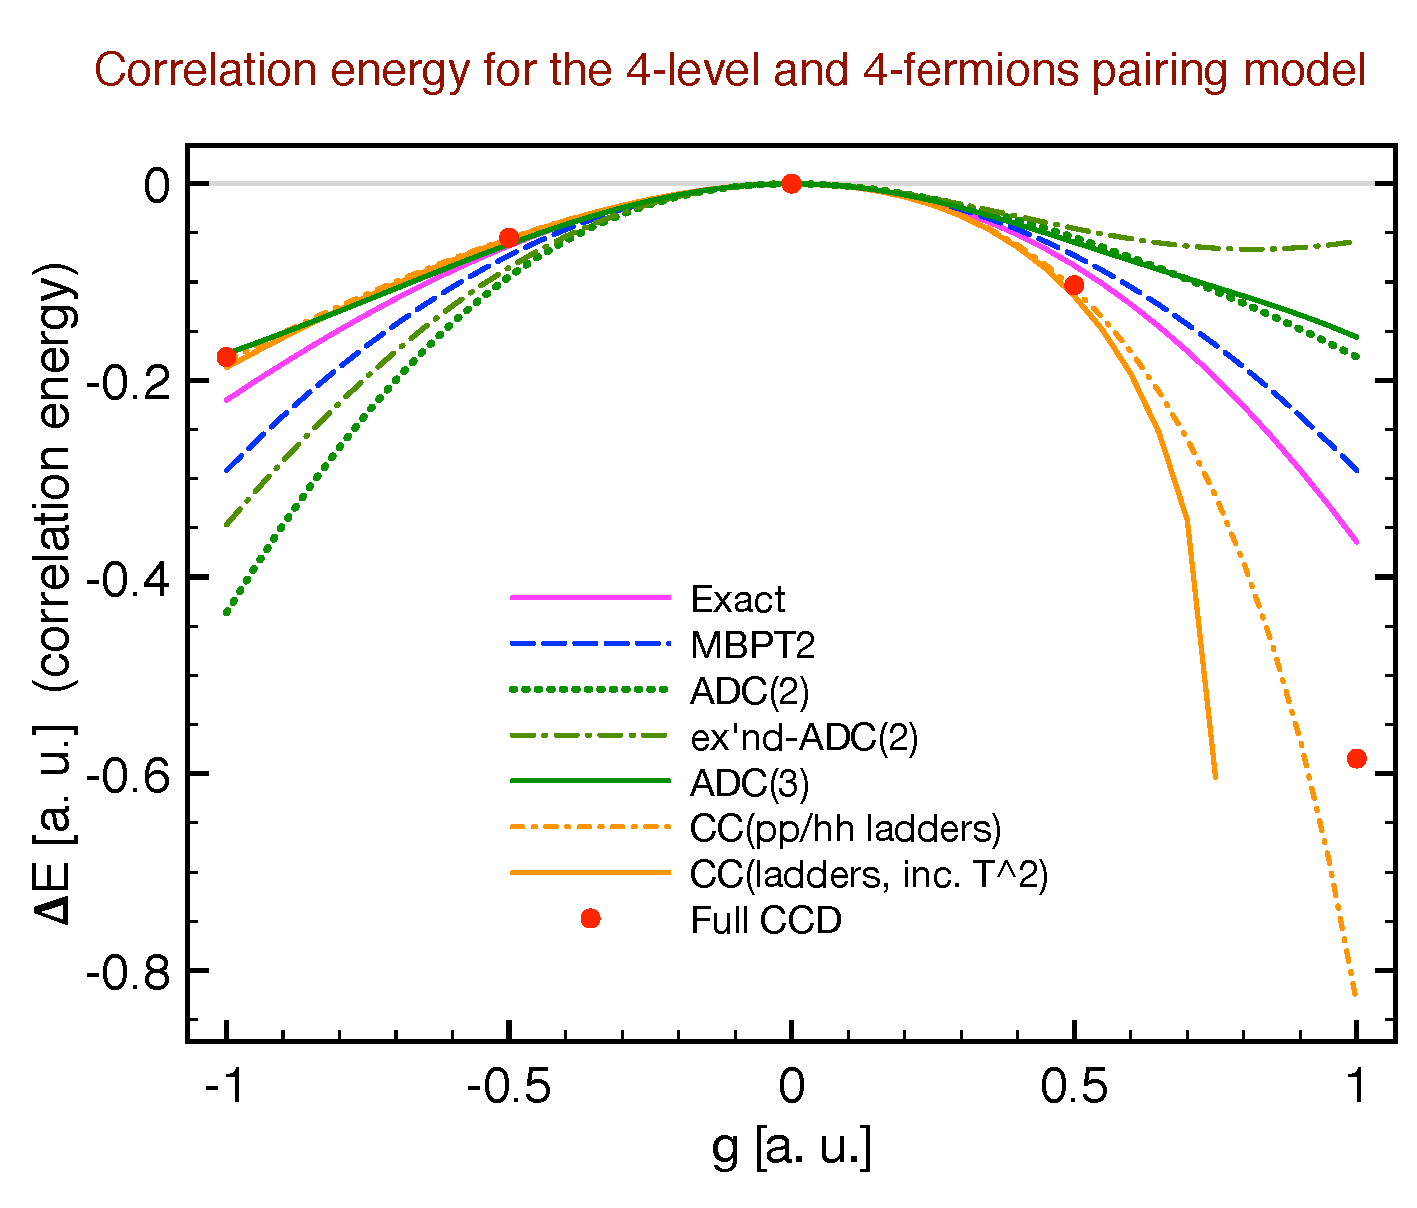
\includegraphics[width=0.8\textwidth]{Chapter11-figures/Pairing_model_CI_ADC_CC.pdf}
\caption{Feynman diagram representations of the Dyson equation. The diagram on the left represents the first line of 
Eqs.~\eqref{eq:Dyson}, while its conjugate equation (second line) is shown on the left. The single line with an
arrow represents the the unperturbed propagator $g^{(0)}_{\alpha\beta}(\omega)$ and the double line is the fully
dressed propagator $g_{\alpha\beta}(\omega)$ of Eq.~\eqref{eq:g1Leh}.  Both diagrams, when expanded in terms
of $g^{(0)}_{\alpha\beta}(\omega)$, give rise to the same solution for the correlated propagator. } 
\label{fig:DysonEq}
\end{center}
\end{figure}

\begin{figure}[ht]
\begin{center}
%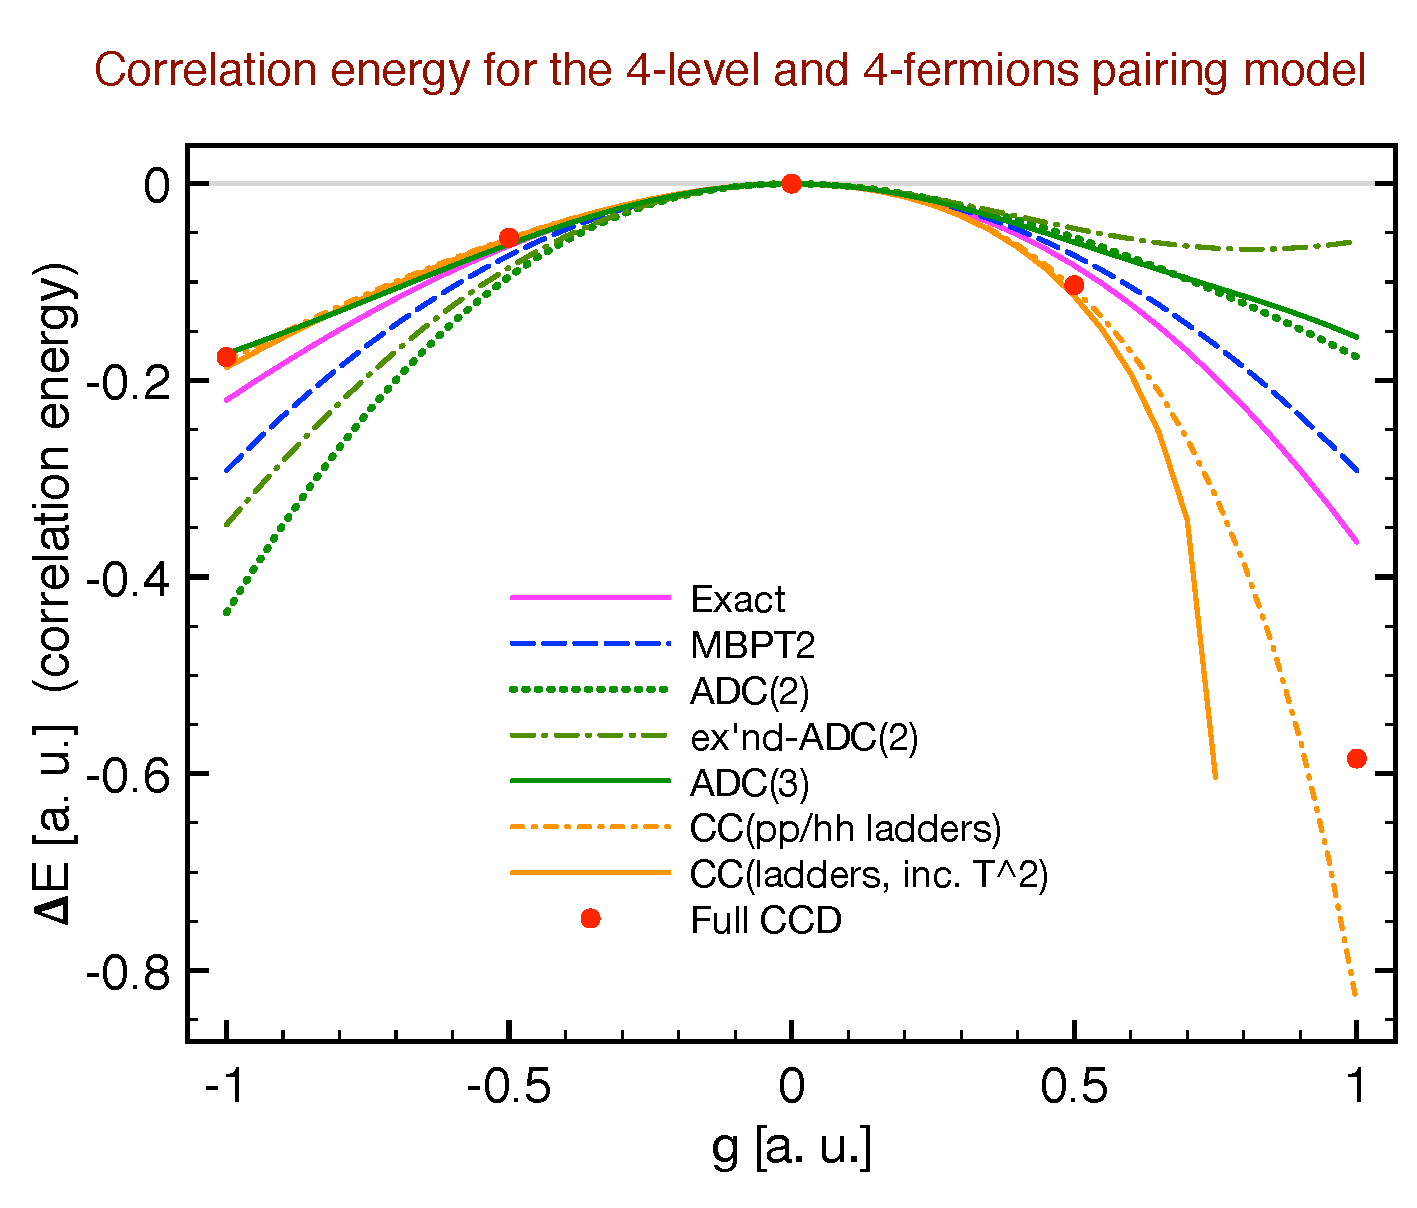
\includegraphics[width=0.8\textwidth]{Chapter11-figures/Pairing_model_CI_ADC_CC.pdf}
\caption{Graphical representation of the effective one- and two-body interactions of Eqs.~\ref{eq:UV_eff}. Dashed lines represent the
one-, two,- and three-body interactions entering Eq.~\eqref{eq:H} and wavy lines are the effective operators $\tilde U$ and  $\tilde V$.}
\label{fig:EffOps}
\end{center}
\end{figure}

\begin{figure}[ht]
\begin{center}
%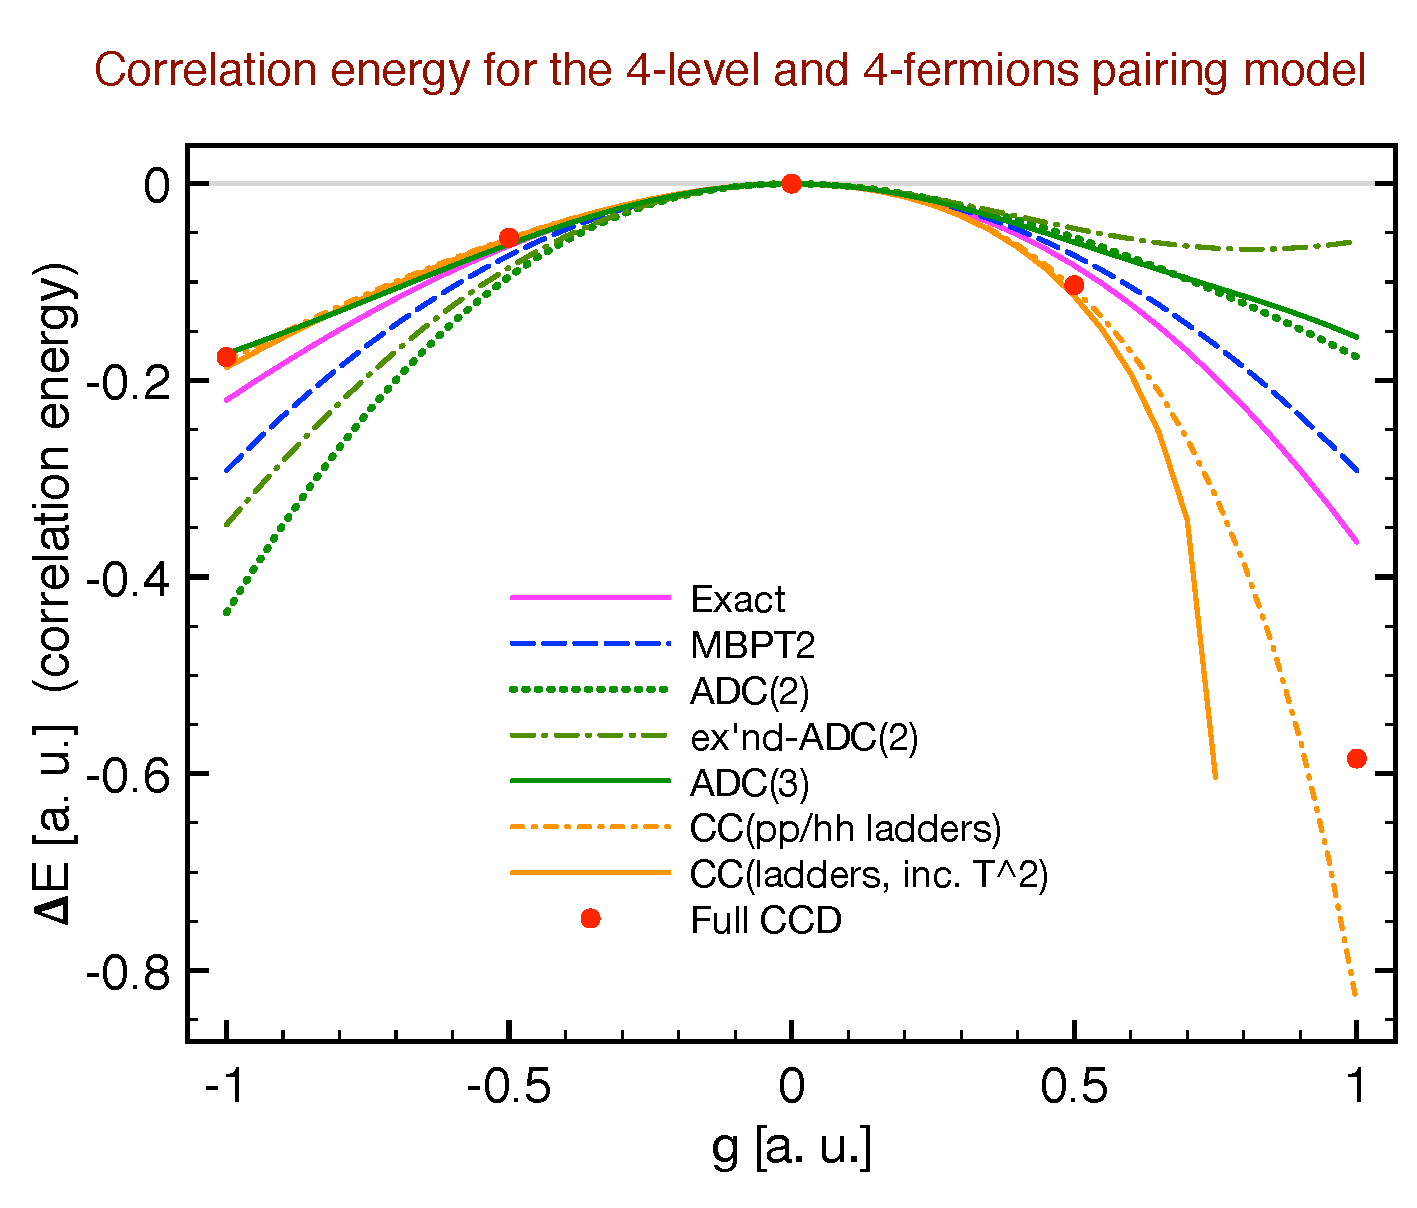
\includegraphics[width=0.8\textwidth]{Chapter11-figures/Pairing_model_CI_ADC_CC.pdf}
\caption{Second order contributions to the self-energy arising from both two- and three-nucleon forces. The diagram depending on the effective two-body interactions (left) also shows the indices and lables used used to calculate its contribution in {\bf Example 11.1}. }
\label{fig:2ndOrd}
\end{center}
\end{figure}

\begin{figure}[ht]
\begin{center}
%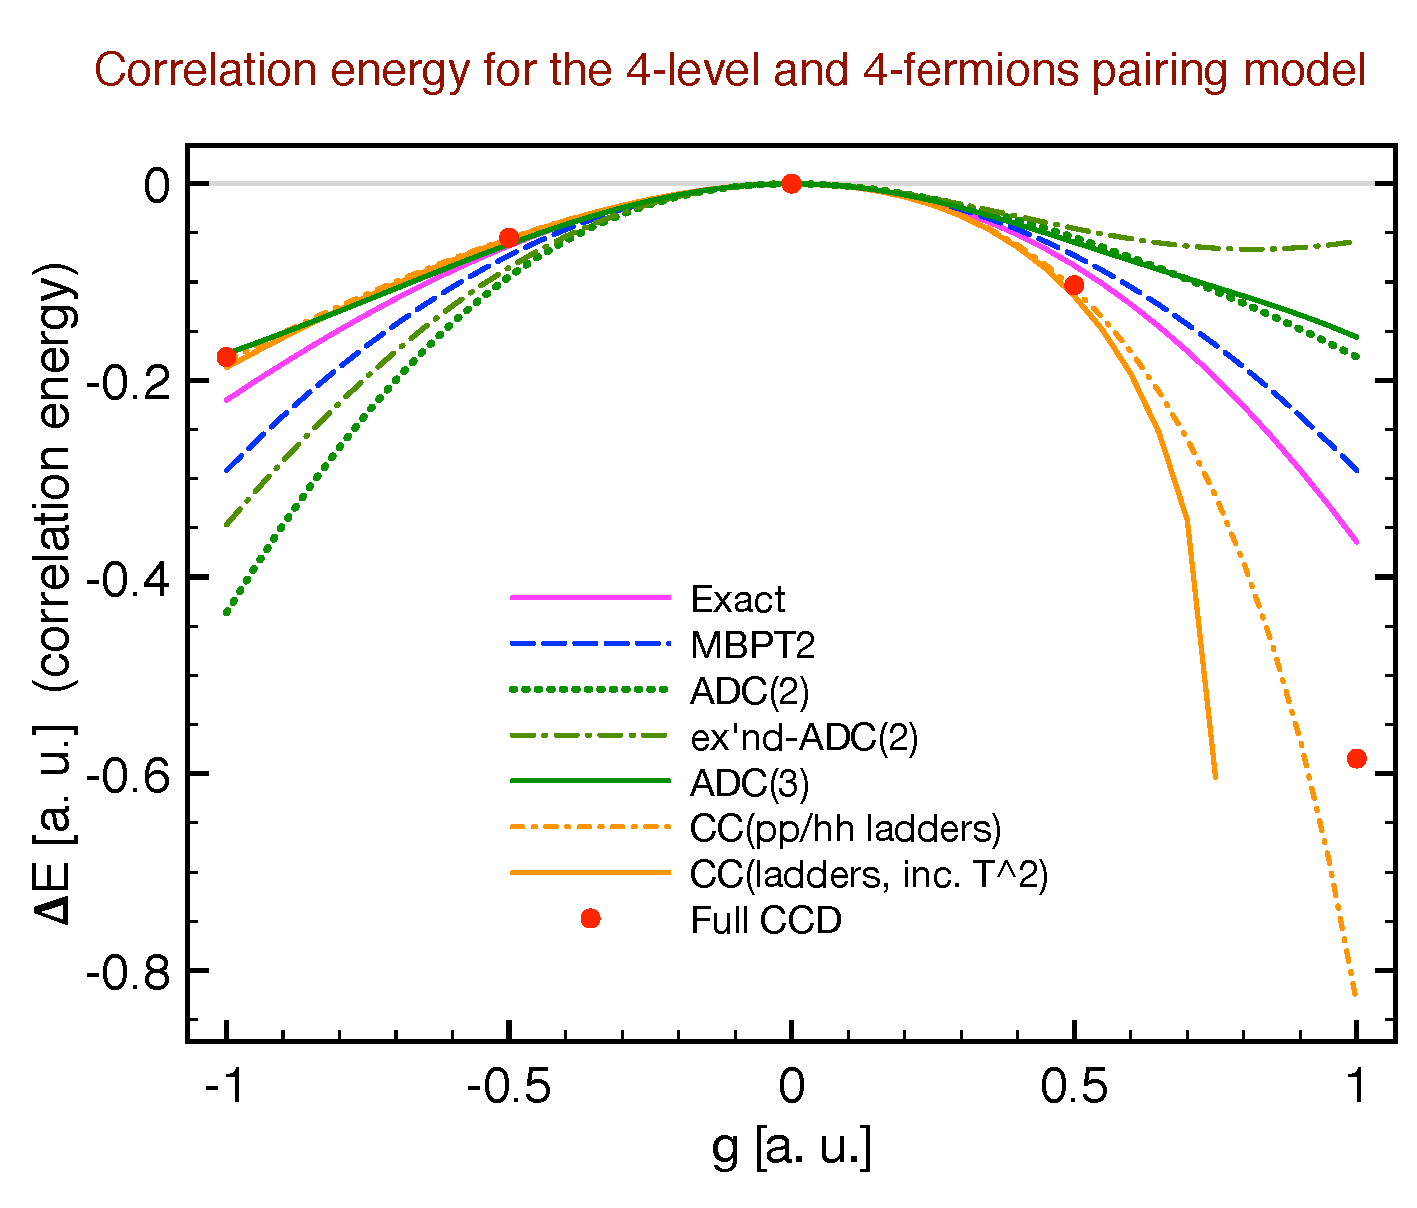
\includegraphics[width=0.8\textwidth]{Chapter11-figures/Pairing_model_CI_ADC_CC.pdf}
\caption{The first two [OR THREE?] skeleton and interaction irreducible diagrams contributing to the self-energy at third order.  All these terms involve intermediate state configurations of at most 2p1h and 2h1p. The first two  
are the only ones containing only two-nucleon interactions and represent the first contribution to ladder (left) and ring (center) resummations. The 
third diagram is the first contribution containing an irreducible three-nucleon interaction. The remaining 14 diagrams at third order all require
explicit three-nucleon interactions and ISC of 3p2h and 3h2p.  }
\label{fig:3rdOrd}
\end{center}
\end{figure}


\subsection{Spectral function and relation to  experimental observations}
\label{sec:scgf_obs}

{\color{blue}
[Here we summarize the spectral function and its relation to one- body observables, the den- sity matrix ?(r) and modification to the Koltun sum rule in presence of 3NFs.]
}


The attractive feature of the SCGF approach is that $g_{\alpha\beta}(\omega)$ describes the one-body dynamics completely. The particle and hole spectral functions are extracted directly from Eq.~\eqref{eq:g1Leh}, respectively:
 \begin{eqnarray}
\nonumber 
S^{p}_{\alpha \beta}(\omega)&=&\sum_{n} \left({\pazocal X}^n_\alpha \right)^*  {\pazocal X}^n_\beta ~ \delta\Big(\omega-(E^{A+1}_n - E^A_0)\Big) \; ,
\\
 \label{eq:SpSh}
S^{h}_{\alpha \beta}(\omega)&=&\sum_{k}  {\pazocal Y}^k_\alpha  \left({\pazocal Y}^k_\beta \right)^* ~\delta\Big(\omega-(E^A_0 - E^{A-1}_k)\Big) \; .
\end{eqnarray} 
The energy distribution of spectroscopic factors is given by
\begin{eqnarray}
  S(\omega) &=& ~ \sum_\alpha S^p_{\alpha \alpha}(\omega) \quad + \quad \sum_\alpha S^h_{\alpha \alpha}(\omega)  \nonumber \\
          &=& ~ \sum_n  SF_n^+ \, \delta( \omega - E^{A+1}_n + E^A_0) 
          ~+~  \sum_n  SF_k^- \, \delta( \omega - E^A_0 + E^{A-1}_k ) \; ;
\label{eq:SFvsE}
\end{eqnarray}
here each peak corresponds to eigenstate of a neighbouring odd-even isotope, whose energy is directly observed in nucleon addition and removal experiments.
Any one-body observable can be calculated via the one-body density matrix $\rho_{\alpha\beta}$, which is obtained from $g_{\alpha\beta}$ as follows:
\begin{equation}
  \label{eq:rho}
  \rho_{\alpha \beta} ~\equiv ~ \langle\Psi_0^A\vert a^{\dag}_{\beta}a_{\alpha} \vert\Psi_0^A\rangle\nonumber\\
  ~=~  \int_{-\infty}^{\varepsilon^-_0}S^h_{\alpha\beta}(\omega)~d\omega=\sum_k ({\pazocal Y}^k_{\beta})^*{\pazocal Y}^k_{\alpha} .
\end{equation}
The expectation value of a one-body operator, ${\hat O}^{1B}$, can then be written in terms of the ${\pazocal Y}$ amplitudes as:
\begin{equation}
\label{eq:den_one}
\langle {\hat O}^{1B}\rangle  =\sum_{\alpha\beta}  O^{1B}_{\alpha \beta}\,\,\rho_{\beta\alpha}=\sum_k \sum_{\alpha\beta}~ ({\pazocal Y}^k_{\alpha})^*~ O^{1B}_{\alpha,\beta} ~  {\pazocal Y}^k_{\beta} \; .
\end{equation}
Evaluating two- and many-nucleon observables requires the knowledge of many-body propagators. In the following, we do this by approximating the corresponding A-body density matrices with A correlated but non-interacting propagators, Eq.~\eqref{eq:rho}.

The exact one-body propagator, $g_{\alpha\beta}(\omega)$, also allows calculating the total energy by means of the extended Koltun sum-rule \cite{Carbone2013Nov}: 
\begin{equation}
  \label{eq:Koltun_hW}
  E^A_0 = \sum_{\alpha\beta} \frac{1}{2} 
            \int_{-\infty}^{\varepsilon^-_0}  [\,T_{\alpha\beta}+\omega\,\delta_{\alpha\beta}\, ]
            S^h_{\beta\alpha}(\omega) d\omega
            -  \frac{1}{2} \langle W\rangle \, .
\end{equation}
This requires only the additional evaluation of the expectation value of the three-nucleon interaction,~$\langle W \rangle$. Again, we approximate this in terms of non-interacting three-body density matrices:
\begin{equation}
   \label{eq:Wddd}
    \langle W\rangle\simeq\frac{1}{6} \, \sum_{\alpha\beta\mu\gamma\delta\nu} W_{\alpha\beta\mu,\gamma\delta\nu}~\rho_{\gamma\alpha}~\rho_{\delta\beta}~\rho_{\nu\mu} \; .
\end{equation}
%
The errors in this approximation have been estimated in Ref.~\cite{Cipollone2013prl} and were found to not exceed the 250~keV on the total binding energy for $^{16}$O and $^{24}$O.

\subsection{Perturbation expansion of the Green 's function}
\label{sec:pertexp}

{\color{blue}
[In order to understand the following sections and to devise appropriate approximations to the self-energy, in is necessary to understand the basics elements of perturbation theory. These will be also fundamental to derive all-order summation schemes leading to non perturbative solutions and to discuss the concept of self-consistency.
We summarize here the material needed to understand the following sections, while the full set of Feynman rules is reviewed in Appendix 2]
}

In order to understand the following sections and to devise appropriate approximations to the self-energy $\Sigma^{\star}(\omega)$, in is necessary to understand the basics elements of perturbation theory.  These will be also fundamental to derive all-order summation schemes leading to non perturbative solutions and to discuss the concept of self-consistency. We summarize here the material needed to understand the following sections, while the full set of Feynman rules is reviewed in  Appendix 2.

We work with a system of $N$ non-relativistic fermions interacting by means of two-body and three-body interactions.
We divide the Hamiltonian into two parts, $\hat H = \hat H_0 + \hat H_1$. 
$\hat H_0 = \hat T + \hat U$ is an unperturbed, one-body contribution. It is 
the sum of the kinetic term and an auxiliary one-body operator, $\hat U$, which defines the reference 
state for the perturbative expansion, $\vert\Phi_0^N\rangle$, on top of which correlations will be added
\footnote{A typical choice in nuclear physics would be a Slater determinant of single-particle harmonic oscillator or a Woods-Saxon wave functions.}.  
The second term of the Hamiltonian, 
$\hat H_1 = -\hat U + \hat V + \hat W$, includes the interactions. $\hat V$ and $\hat W$ denote, respectively, the two-body and three-body interaction operators.
In a second-quantised framework, the full Hamiltonian reads:
\begin{equation}
\label{eq:H}
\hat H = \sum_{\alpha} \varepsilon^0_\alpha\, a^\dag_\alpha a_\alpha - \sum_{\alpha\beta}U_{\alpha,\beta}\, a^\dag_\alpha a_{\beta}
%\\\nonumber &+&
+\frac{1}{4} \sum_{\substack{\alpha\gamma\\\beta\delta}}V_{\alpha\gamma,\beta\delta}\, a_\alpha^\dag a_\gamma^\dag a_{\delta} a_{\beta}
%\\\nonumber &+& 
+\frac{1}{36}\sum_{\substack{\alpha\gamma\epsilon \\ \beta\delta\eta}} W_{\alpha\gamma\epsilon,\beta\delta\eta}\,
a_\alpha^\dag a_\gamma^\dag a_\epsilon^\dag a_{\eta} a_{\delta} a_{\beta} \, .
\end{equation}
The greek indices $\alpha$,$\beta$,$\gamma$,\ldots label a complete set of SP states which diagonalize the unperturbed Hamiltonian, $\hat H_0$, with eigenvalues $\varepsilon_\alpha^0$. 
$a^\dag_\alpha$ and $a_\alpha$ are creation and annihilation operators for a particle in state $\alpha$. 
The matrix elements of the one-body operator $\hat U$ are given by $U_{\alpha,\beta}$. Equivalently, the matrix elements of the
two-body and three-body forces are $V_{\alpha\gamma,\beta\delta}$ and $W_{\alpha\gamma\epsilon,\beta\delta\eta}$. 
In the following, we work with antisymmetrized matrix elements in both the two-body and the three-body sectors.

In time-space, the one-body propagator is defined as the expectation value of the time-ordered product of an annihilation and a creation operators in the Heisenberg picture, which Fourier transformed gives its Lehman representation given in Eq.~(\ref{eq:g1Leh}). Interactions in the many-body system can be treated by means of a perturbative expansion. 
For the one-body propagator this expansion reads \cite{Mattuck1992,Dickhoff2008}:
\begin{equation}
\label{gpert}
g_{\alpha\beta}(t_\alpha-t_\beta) = -\frac{\rm i}{\hbar} \sum_{n=0}^\infty \left(-\frac{\rm i}{\hbar}\right)^n\frac{1}{n!}\int \hspace{-1mm} {\rm d} t_1 \; \ldots \int \hspace{-1mm} {\rm d} t_n \langle\Phi_0^N\vert {\pazocal T} [\hat H_1(t_1) \ldots \hat H_1(t_n)a^I_\alpha(t_\alpha){a_{\beta}^I}^\dag(t_\beta)]\vert\Phi_0^N\rangle_\text{conn} \; ,
\end{equation}
where $a^I_\alpha$ and ${a_{\beta}^I}^\dag$ are now operators in the interaction picture with respect to $H_0$. 
The subscript ``conn'' implies that only \emph{connected} diagrams have to be considered when performing
the Wick contractions of the time-ordered product ${\pazocal T}$. $H_1$ contains contributions from one-body, two-body and three-body interactions. Thus, the expansion involves terms with individual contributions of each force, as well as combinations of these. 
Feynman diagrams are essential to keep track of such a variety of different contributions.
The set of Feynman diagrammatic rules that stems out of Eq.~(\ref{gpert}) in the presence of three-body interactions
is reviewed in detail in Appendix 2.

A first reorganisation of the contributions generated by Eq.~(\ref{gpert}) is obtained by considering 
\emph{one-particle reducible} diagrams, i.e. diagrams that can be disconnected by cutting a single fermionic line. 
Reducible diagrams are generated by an all-orders summation through Dyson's equation~(\ref{eq:Dyson}). Thus, in practice, one only needs to include \emph{one-particle irreducible} (1PI) contributions
to the self-energy, $\Sigma^\star$. 
The uncorrelated SP propagator, $g^{(0)}$ appearing in Eq.~(\ref{eq:Dyson}), is associated with the system governed by the $H_0$ Hamiltonian 
and represents the $n=0$ order in the expansion of Eq.~(\ref{gpert}). The irreducible self-energy $\Sigma^\star$ describes the kernel of all 1PI diagrams.
This operator plays a central role in the GF formalism and can be interpreted as the 
non-local and energy-dependent interaction that each fermion feels due to the interaction with the medium. 
At positive energies, $\Sigma^\star(\omega)$ is also identified with the optical potential for scattering of a particle 
from the many-body target. 

A further level of simplification in the self-energy expansion 
can be obtained if unperturbed propagators, $g^{(0)}$, in the internal fermionic lines are replaced by dressed Green's functions, $g$. 
This process is generically called propagator renormalization and 
further restricts the set of diagrams to \emph{skeleton} diagrams \cite{Dickhoff2008}.
These are defined as 1PI diagrams that do not contain 
any portion that can be disconnected by cutting a fermion line twice at any two different points. 
These portions would correspond to self-energy insertions, which are already re-summed into the dressed propagator $G$ by Eq.~(\ref{eq:Dyson}).
The SCGF approach is precisely based on diagrammatic expansions of such skeleton diagrams 
with renormalized propagators.

In principle, this framework offers great advantages. First, it is intrinsically nonperturbative and completely
independent from any choice of the reference state and auxiliary one-body potential, $\hat{U}$, 
which automatically drops out of Eq.~(\ref{eq:Dyson}). 
Second, many-body correlations are expanded directly in terms of SP excitations which are closer
to the exact solution than those associated with the unperturbed state, $\vert\Phi_0^N\rangle$. Third, 
the number of diagrams is vastly reduced to 1PI skeletons. 
Fourth, a full SCGF calculation automatically satisfies the basic conservation
laws~\cite{Baym1961,Baym1962,Dickhoff2008}. 

It is possible to further restrict the set of relevant diagrams by
exploiting the concept of \emph{effective interactions}~\cite{Carbone2013Nov}. Hence, for a system with up to 3BFs, we define an effective Hamiltonian,
\begin{equation}
\widetilde H_1= {\widetilde U} + {\widetilde  V} + \hat W \,
\label{Heff}
\end{equation}
where $\widetilde U$ and  $\widetilde V$ represent effective interaction operators. 
The diagrammatic expansion arising from  Eq.~(\ref{gpert}) with the effective Hamiltonian $\widetilde H_1$ is
formed only of (1PI, skeleton) interaction-irreducible diagrams to avoid any possible double counting.
Note that the three-body interaction, $\hat W$, remains the same as in Eq.~\eqref{eq:H} but enters only the 
interaction-irreducible diagrams with respect to three-body interactions.
The explicit expressions for the one-body and two-body effective interaction operators are:
\begin{align}
  \label{eq:UV_eff}
  \widetilde{U}_{\alpha\beta}&= ~ ~ U_{\alpha\beta}  ~ ~ +  ~\sum_{\delta\gamma} V_{\alpha\gamma,\beta\delta}~\rho_{\delta\gamma}
                        ~ +  ~ \frac{1}{4} \sum_{\mu \nu \gamma \delta}W_{\alpha\mu\nu,\beta\gamma\delta}~\rho_{\gamma\mu}~\rho_{\delta\nu}  \; ,
  \nonumber \\
  \widetilde{V}_{\alpha\beta,\gamma\delta} &= ~ V_{\alpha\beta,\gamma\delta}  ~+ ~ 
                          \sum_{\mu\nu}W_{\alpha\beta \mu ,\gamma \delta \nu}~\rho_{\nu\mu}  \; .
\end{align}
The effective Hamiltonian of Eq.~(\ref{Heff})  not only regroups Feynman diagrams in 
a more efficient way, but also defines the effective 1B and 2B terms from 
higher order interactions. As long as interaction-irreducible diagrams are used together with the 
effective Hamiltonian, $\widetilde{H}_1$, this approach provides a systematic
way to incorporate many-body forces in the calculations and to 
generate effective in-medium interactions. More importantly, the formalism is such that 
symmetry factors are properly considered and no diagram is over-counted. This approach can be seen as a generalisation of the normal
ordering of the Hamiltonian with respect to the reference state $\vert\Phi_0^N\rangle$, however, the contraction goes beyond normal ordering
because it is performed with respect to the exact
correlated density matrices. To some extent, one can think of 
the effective Hamiltonian, $\widetilde{H}$,  as being reordered with respect
to the interacting many-body ground-state $|\Psi_0^N\rangle$, rather than 
the non-interacting  $\vert\Phi_0^N\rangle$. 

All interaction-irreducible contributions to the proper self-energy up to third order in perturbation theory can be found in Ref.~\cite{Carbone2013Nov}. There, an overview of how the approach can be extended to higher-order perturbative and also to nonperturbative calculations is presented in detail.

\vskip 0.3 cm
\noindent
{\bf Example 11.1} Calculate the Feynman-Galitskii propagator that corresponds to the propagation of two particles or two holes that do not interac with each other.

This is a  two-body propagator and therefore an extension of Eq.~\eqref{eq:g1Time}. Let us we label  the two initial states with indices $\gamma$ and $\delta$ and that the two final states with $\alpha$ and $\beta$. We then take the case when the particle in state $\gamma$ propagates directly into $\alpha$ (and therefore $\delta$ independently propagates into $\beta$).  Using the perturbation expansion analogous to Eqs.~\ref{gpert} to zeroth-order, or the Feynman rules reported in Appendix~\ref{app:Feyn_rules}, we obtain:
\begin{eqnarray}
G^{II,f}_{\alpha \beta, \gamma \delta}(\omega) &=& (i\hbar)^{-1} \int \frac {d \omega_1}{2\pi} 
  \; i\hbar \,  g_{\alpha\gamma}(\omega-\omega_1) \; i\hbar \, g_{\beta\delta}(\omega_1)
\label{eq:GIIf_int} \\ \nonumber
&=& - \int \frac {d \omega_1}{2\pi}  
  \left\{ \frac{(\pazocal{X}^{n_1}_\alpha)^*  \pazocal{X}^{n_1}_\gamma}{\omega - \omega_1  - e^+_{n_1} + i\eta} 
        + \frac{\pazocal{Y}^{k_1}_\alpha  (\pazocal{Y}^{k_1}_\gamma)^*}{\omega - \omega_1  - e^-_{k_1} - i\eta}  \right\}
          \left\{ \frac{(\pazocal{X}^{n_2}_\beta)^*  \pazocal{X}^{n_2}_\delta}{\omega_1  - e^+_{n_2} + i\eta} 
        + \frac{\pazocal{Y}^{k_2}_\beta  (\pazocal{Y}^{k_2}_\delta)^*}{\omega_1  - e^-_{k_2} - i\eta}  \right\} \, ,
\end{eqnarray}
where we have have used the convention that repeated indices are summed over. The integral in the above equation can be performed with the Cauchy theorem by closing ark on either the positive od the negative imaginary half planes. Hence, contributions where all the poles are  on the same side of the real axis cancel out. Extracting the residues of the other terms leads to the following result:
\begin{equation}
G^{II,f}_{\alpha \beta, \gamma \delta}(\omega) =
\sum_{n_1, \, n_2} \frac{(\pazocal{X}^{n_1}_\alpha \pazocal{X}^{n_2}_\beta)^*  \pazocal{X}^{n_1}_\gamma \pazocal{X}^{n_2}_\delta}
                      {\omega  - (e^+_{n_1}  + e^+_{n_2}) + i\eta} 
~-~ \sum_{k_1, \, k_2} \frac{\pazocal{Y}^{k_1}_\alpha \pazocal{Y}^{k_2}_\beta \, (\pazocal{Y}^{k_1}_\gamma \pazocal{Y}^{k_2}_\delta)^*}
                     {\omega  - (e^-_{k_1} + e^-_{k_2}) - i\eta}   \; .
\label{eq:GIIf}
\end{equation}

\vskip 0.3 cm
\noindent
{\bf Example 11.2} Calculate the expression for the second order contribution to $\Sigma^\star$ from two-nucleon interactions only.

This is the first diagram (on the left) of Fig.~\ref{fig:2ndOrd}. By applying Feynman rules we have:
\begin{eqnarray}
 \Sigma^{(2,2N)}_{\alpha\beta}(\omega) &=&
  - \frac{(i\hbar)^2}{2} \int \frac {d \omega_1}{2\pi} \frac {d \omega_2}{2\pi}  V_{\alpha\sigma,\gamma\delta} 
         \,  g_{\gamma\mu}(\omega+\omega_2-\omega_1) \, g_{\delta\nu}(\omega_1) \, g_{\lambda\sigma}(\omega_2) 
           \, V_{\mu \nu, \beta \lambda}
\nonumber \\
   &=& + \frac{1}{2} \int \frac {d \omega_2}{2\pi} V_{\alpha\sigma,\gamma\delta} \; 
     G^{II,f}_{\gamma \delta, \mu \nu}(\omega+\omega_2)   \, g_{\lambda\sigma}(\omega_2) 
           \, V_{\mu \nu, \beta \lambda}
\nonumber \\
  &=& \frac{1}{2}   \int \frac {d \omega_2}{2\pi} \, V_{\alpha\sigma,\gamma\delta} \,
  \left\{
    \frac{(\pazocal{X}^{n_1}_\gamma \pazocal{X}^{n_2}_\delta)^*  \pazocal{X}^{n_1}_\mu \pazocal{X}^{n_2}_\nu}
                      {\omega  - (e^+_{n_1}  + e^+_{n_2}) + i\eta} 
 -  \frac{ \pazocal{Y}^{k_1}_\gamma \pazocal{Y}^{k_2}_\delta \, (\pazocal{Y}^{k_1}_\mu \pazocal{Y}^{k_2}_\nu)^*}
                     {\omega  - (e^-_{k_1} + e^-_{k_2}) - i\eta}
  \right\}
\nonumber \\
&& \qquad \qquad \quad \times  \left\{ \frac{(\pazocal{X}^{n_3}_\lambda )^* \pazocal{X}^{n_3}_\sigma}{\omega_1 - \omega  - e^+_{n_3} + i\eta} 
        + \frac{\pazocal{Y}^{k_3}_\lambda  (\pazocal{Y}^{k_3}_\sigma)^*}{\omega_1 - \omega  - e^-_{k_3} - i\eta}  \right\} 
          \, V_{\mu \nu, \beta \lambda}
 \; .
\end{eqnarray}
Note that the  integration over $d \omega_1$ is exactly the same as in Eq.~\eqref{eq:GIIf_int}. Thus, we can directly substitute the expression for the Feynman-Galitskii propagator~\eqref{eq:GIIf}  in the last two lines above. By performing the last Cauchy integral we obtain the final result for the second order irreducible self-energy: 
\begin{equation}
\Sigma^{(2,2N)}_{\alpha\beta}(\omega) = \frac{1}{2}  V_{\alpha\sigma,\gamma\delta} \left\{
   \sum_{\substack{n_1, \, n_2 \\  k_3}} \frac{(\pazocal{X}^{n_1}_\gamma   \pazocal{X}^{n_2}_\delta    \pazocal{Y}^{k_3}_\sigma)^*
                                                      \pazocal{X}^{n_1}_\mu \pazocal{X}^{n_2}_\nu  \pazocal{Y}^{k_3}_\lambda}
                      {\omega  - (e^+_{n_1}  + e^+_{n_2}- e^-_{k_3}) + i\eta} 
+ \sum_{\substack{k_1, \, k_2 \\ n_3}} \frac{\pazocal{Y}^{k_1}_\gamma     \pazocal{Y}^{k_2}_\delta \pazocal{X}^{n_3}_\sigma \, 
                                                       (\pazocal{Y}^{k_1}_\mu \pazocal{Y}^{k_2}_\nu \pazocal{X}^{n_3}_\lambda )^*}
                     {\omega  - (e^-_{k_1} + e^-_{k_2}- e^+_{n_3}) - i\eta}  
       \right\}  V_{\mu \nu, \beta \lambda} \; ,
\label{eq:Sig_2nd}
\end{equation}
where repeated greek indices are summed over implicitly but we show the explicit summation of the poles corresponding to 2p1h and 2h1p intermediate state configurations (ISC).



\vskip 0.3 cm
\noindent
{\bf Exercise 11.1} Calculate the expression for the  the second order contribution to $\Sigma^\star(\omega)$ arising from three-nucleon interactions (diagram on the right side of Fig.~\ref{fig:2ndOrd}). Show that this contains ISC of 3p2h and 3h2p.

\vskip 0.3 cm
\noindent
{\bf Solution} Upon performing the four frequency integral, one obtains:
\begin{eqnarray}
\Sigma^{(2,3N)}_{\alpha\beta}(\omega) &=& \frac{1}{2}  W_{\alpha\gamma\delta, \mu\nu\lambda} \left\{
   \sum_{\substack{n_1, \, n_2 ,\, n3 \\  k_4,\, k_5}} 
       \frac{(\pazocal{X}^{n_1}_\mu   \pazocal{X}^{n_2}_\nu   \pazocal{X}^{n_3}_\lambda    \pazocal{Y}^{k_4}_\gamma  \pazocal{Y}^{k_5}_\delta)^*
                 \pazocal{X}^{n_1}_{\mu'} \pazocal{X}^{n_2}_{\nu'}  \pazocal{X}^{n_3}_{\lambda'}    \pazocal{Y}^{k_4}_{\gamma'} \pazocal{Y}^{k_5}_{\delta'}}
                      {\omega  - (e^+_{n_1}  + e^+_{n_2} + e^+_{n_3}- e^-_{k_4}- e^-_{k_5}) + i\eta} 
 \right. \nonumber \\
 &&\qquad \qquad \qquad \qquad \left. +
\sum_{\substack{k_1, \, k_2 ,\, k_3 \\ n_4 ,\ n_5}} 
         \frac{\pazocal{Y}^{k_1}_\mu     \pazocal{Y}^{k_2}_\nu    \pazocal{Y}^{k_3}_\lambda \pazocal{X}^{n_4}_\gamma \pazocal{X}^{n_5}_\delta \, 
               (\pazocal{Y}^{k_1}_{\mu'} \pazocal{Y}^{k_2}_{\nu'}     \pazocal{Y}^{k_3}_{\lambda'} \pazocal{X}^{n_4}_{\gamma'} \pazocal{X}^{n_5}_{\delta'} )^*}
                     {\omega  - (e^-_{k_1} + e^-_{k_2}+ e^-_{k_3}- e^+_{n_4}- e^+_{n_5}) - i\eta}  
       \right\}  W_{\mu' \nu' \lambda' , \beta \gamma' \delta'} \, . \qquad \qquad
\label{eq:Sig_2nd_3b}
\end{eqnarray}



\section{The Algebraic Diagrammatic Construction method}
\label{sec:scgf_adc}

The general Lehman representation of the self-energy is given by~\eqref{}, where $\Sigma^{(\infty)}$  is given by the mean-field diagram of Fig.~\ref{}. Similarly to the case of a propagator, Eqs.~\eqref{eq:g1Leh} and~\eqref{eq:Sig_2nd}, the  pole structure of the energy-dependent part is dictated by the principle of causality with the correct boundary conditions coded by the  $\pm i\eta$ terms at the denominators.  This implies a dispersion relation that  can links the real and imaginary parts of the self-energy~\cite{Dickhoff2008}.  Correspondingly, the direct coupling of single particle orbits to  ISCs (of 2p1h and 2h1p character or more complex) imposes  the separable structure of the residues. In this section we consider that case of a  finite system, for which it is useful to use a discretised single particle basis as a model space. Thus, the above constraints impose the following  analytical form the the self-energy operator:
\begin{equation}
\Sigma^{(\star)}_{\alpha\beta}(\omega) = \Sigma^{(\infty)}_{\alpha\beta} +M^\dagger_{\alpha,r}\frac1{\omega - [E +C]_{r,r'} + i \eta}M_{r',\beta} 
       +N_{\alpha,s}\frac1{\omega - [E +D]_{s,s'} - i \eta}N^\dagger_{s',\beta}  \; ,
\label{eq:ADC_SE_form}
\end{equation}
where $r$ and $s$ are collective indices that label sets of configurations beyond single particle structure. Specifically, $r$ is for particle addition and will label 2p1h, 3p2h, 4p3h, ... states, in the general case. Likewise, $s$ is for particle removal and we will used it to label 2h1p states (or higher configurations). However, for the approximations presented here and for our discussion below we will only be limited to 2p1h and 2h1p ISCs.

The expansion of the self-energy at second order in perturbation theory trivially satisfies Eq.~\eqref{eq:ADC_SE_form}. By simple comparison with the results  of Eq.~\eqref{eq:Sig_2nd} shows us that the sums over $r$ and $s$ can be taken to cover the configurations $r\equiv\{n_1 < n_2,k_3\}$ and  $s\equiv\{k_1 < k_2, n_3\}$. Thus, we can identify the expressions for the matrix elements of the residues and poles as follows:
\begin{eqnarray}
 M_{\alpha,r} &=& %\sum_{\mu \nu \lambda}
     \pazocal{X}^{n_1}_\mu \pazocal{X}^{n_2}_\nu  \pazocal{Y}^{k_3}_\lambda  V_{\mu \nu, \beta \lambda}
 \nonumber \\
 E_{r,r'} &=& diag \left\{ \,\varepsilon^+_{n_1} + \varepsilon^+_{n_2} - \varepsilon^-_{k_3}  \, \right\}
 \nonumber \\
 C_{r,r'} &=& 0
 \label{eq:ADC2_MC}
   \\
 N_{\alpha,s} &=& \pazocal{Y}^{k_1}_\mu \pazocal{Y}^{k_2}_\nu \pazocal{X}^{n_3}_\lambda  V_{\mu \nu, \beta \lambda}
 \nonumber \\
 E_{s,s'} &=& diag \left\{ \, \varepsilon^-_{k_1} + \varepsilon^-_{k_2} - \varepsilon^+_{n_3} \, \right\} 
 \nonumber \\
 D_{s,s'} &=& 0
  \label{eq:ADC2_ND}
\end{eqnarray}
where the factor $1/2$ from Eq.~\eqref{eq:Sig_2nd} disappears since we restrict the sums to triplets of indices where  $n_1<n_2$ and $k_1<k_2$.
As we discuss below, Eqs~.\eqref{eq:ADC2_MC} and \eqref{eq:ADC2_ND}, define the algebraic diagrammatic method
at second order [ADC(2)].


Unfortunately, $\Sigma^\star(\omega)$ loses its analytical form, Eq.~\eqref{eq:ADC_SE_form}, as soon as one moves to higher orders in perturbation theory. To demonstrated this, let us calculate the contribution of the third order 'ladder' diagram of Fig.~\ref{fig:3rdOrd}. By exploiting Feynman rules
and Eq.~\eqref{eq:GIIf_int} we obtain
\begin{eqnarray}
  \Sigma^{(3,ld)}_{\alpha\beta}(\omega) &=& - \frac{i^3}{4} \int \frac{d\omega_1}{2\pi} \int \frac{d\omega_2}{2\pi} \int \frac{d\omega_3}{2\pi} 
  V_{\alpha\sigma,\gamma\delta} 
         \,  g_{\gamma\gamma'}(\omega+\omega_3-\omega_1) \, g_{\delta\delta'}(\omega_1) 
           \, V_{\gamma' \delta', \mu' \nu'}
  \nonumber \\ && \qquad \qquad \qquad \qquad \qquad \qquad \qquad \qquad \times
    \,  g_{\mu'\mu}(\omega+\omega_3-\omega_2) \, g_{\nu'\nu}(\omega_2) \, V_{\mu \nu, \beta \lambda} \,  g_{\lambda\sigma}(\omega_3) 
\nonumber \\
  &=&  \frac{1}{4}  \int \frac{d\omega_3}{2\pi i} 
  V_{\alpha\sigma,\gamma\delta} 
         \,  G^{II,f}_{\gamma\delta, \gamma' \delta'}(\omega+\omega_3) \,  
           \, V_{\gamma' \delta', \mu' \nu'}     \,  G^{II,f}_{\mu' \nu', \mu \nu}(\omega+\omega_3) \, V_{\mu \nu, \beta \lambda}  \, g_{\lambda\sigma}(\omega_3) 
\nonumber \\
  &=&  \frac{1}{4}  \int \frac{d\omega_3}{2\pi i} 
    V_{\alpha\sigma,\gamma\delta} \,
  \left\{
    \frac{(\pazocal{X}^{n_1}_\gamma \pazocal{X}^{n_2}_\delta)^*  \pazocal{X}^{n_1}_{\gamma'} \pazocal{X}^{n_2}_{\delta'}}
                      {\omega+\omega_3  - (e^+_{n_1}  + e^+_{n_2}) + i\eta} 
 -  \frac{ \pazocal{Y}^{k_1}_\gamma \pazocal{Y}^{k_2}_\delta \, ( \pazocal{Y}^{k_1}_{\gamma'} \pazocal{Y}^{k_2}_{\delta'})^*}
                     {\omega+\omega_3  - (e^-_{k_1} + e^-_{k_2}) - i\eta}
  \right\}
\nonumber \\
 && \qquad \qquad \times    \, V_{\gamma' \delta', \mu' \nu'} \,  \left\{
    \frac{( \pazocal{X}^{n_4}_{\mu'} \pazocal{X}^{n_5}_{\nu'})^*  \pazocal{X}^{n_4}_\mu \pazocal{X}^{n_5}_\nu}
                      {\omega+\omega_3  - (e^+_{n_4}  + e^+_{n_5}) + i\eta} 
 -  \frac{ \pazocal{Y}^{k_4}_{\mu'} \pazocal{Y}^{k_5}_{\nu'} \, (\pazocal{Y}^{k_4}_\mu \pazocal{Y}^{k_5}_\nu)^*}
                     {\omega+\omega_3  - (e^-_{k_4} + e^-_{k_5}) - i\eta}
  \right\}
 \nonumber \\
 && \qquad \qquad \qquad \qquad \times   V_{\mu \nu, \beta \lambda}
   \left\{ \frac{(\pazocal{X}^{n_3}_\lambda )^* \pazocal{X}^{n_3}_\sigma}{\omega_3  - e^+_{n_3} + i\eta} 
           + \frac{\pazocal{Y}^{k_3}_\lambda  (\pazocal{Y}^{k_3}_\sigma)^*}{\omega_3  - e^-_{k_3} - i\eta}  \right\}   \; .
\label{eq:LaddEg1}
 \end{eqnarray}
Performing the Cauchy integrals, only six term out of the eight combinations of poles survive. To simplify the discussion 
we will focus only on the three integrals that contribute to the forward propagation of the self-energy (second term on the r.h.s.
 of \eqref{eq:ADC_SE_form}). This is done by retaining only the poles $(\omega_3  - e^-_{k_3} - i\eta)^{-1}$ in the
 last propagator of Eq.~\eqref{eq:LaddEg1}, which lie above the real axis with respect to the integrand $\omega_3$. Thus,
 we have:
 \begin{eqnarray}
  \Sigma^{(ld,>)}_{\alpha\beta}(\omega) &=& 
 \frac{1}{4}  \int \frac{d\omega_3}{2\pi i} 
    V_{\alpha\sigma,\gamma\delta} \,
  \left\{
 -  \frac{ \pazocal{Y}^{k_1}_\gamma \pazocal{Y}^{k_2}_\delta \, ( \pazocal{Y}^{k_1}_{\gamma'} \pazocal{Y}^{k_2}_{\delta'})^*}
                     {\omega+\omega_3  - (e^-_{k_1} + e^-_{k_2}) - i\eta}
  \right\}
\nonumber \\
&& \qquad \qquad \times
   \, V_{\gamma' \delta', \mu' \nu'} \,  \left\{
    \frac{( \pazocal{X}^{n_4}_{\mu'} \pazocal{X}^{n_5}_{\nu'})^*  \pazocal{X}^{n_4}_\mu \pazocal{X}^{n_5}_\nu}
                      {\omega+\omega_3  - (e^+_{n_4}  + e^+_{n_5}) + i\eta} 
  \right\}
  V_{\mu \nu, \beta \lambda}
   \left\{  \frac{\pazocal{Y}^{k_3}_\lambda  (\pazocal{Y}^{k_3}_\sigma)^*}{\omega_3  - e^-_{k_3} - i\eta}  \right\}
     \nonumber \\
&&+
 \frac{1}{4}  \int \frac{d\omega_3}{2\pi i} 
    V_{\alpha\sigma,\gamma\delta} \,
  \left\{
    \frac{(\pazocal{X}^{n_1}_\gamma \pazocal{X}^{n_2}_\delta)^*  \pazocal{X}^{n_1}_{\gamma'} \pazocal{X}^{n_2}_{\delta'}}
                      {\omega+\omega_3  - (e^+_{n_1}  + e^+_{n_2}) + i\eta} 
  \right\}
\nonumber \\
&& \qquad \qquad \times
   \, V_{\gamma' \delta', \mu' \nu'} \,  \left\{
 -  \frac{ \pazocal{Y}^{k_4}_{\mu'} \pazocal{Y}^{k_5}_{\nu'} \, (\pazocal{Y}^{k_4}_\mu \pazocal{Y}^{k_5}_\nu)^*}
                     {\omega+\omega_3  - (e^-_{k_4} + e^-_{k_5}) - i\eta}
  \right\}
  V_{\mu \nu, \beta \lambda}
   \left\{  \frac{\pazocal{Y}^{k_3}_\lambda  (\pazocal{Y}^{k_3}_\sigma)^*}{\omega_3  - e^-_{k_3} - i\eta}  \right\}
     \nonumber \\
&&+
 \frac{1}{4}  \int \frac{d\omega_3}{2\pi i} 
    V_{\alpha\sigma,\gamma\delta} \,
  \left\{
    \frac{(\pazocal{X}^{n_1}_\gamma \pazocal{X}^{n_2}_\delta)^*  \pazocal{X}^{n_1}_{\gamma'} \pazocal{X}^{n_2}_{\delta'}}
                      {\omega+\omega_3  - (e^+_{n_1}  + e^+_{n_2}) + i\eta} 
  \right\}
\nonumber \\
&& \qquad \qquad \times
   \, V_{\gamma' \delta', \mu' \nu'} \,  \left\{
    \frac{( \pazocal{X}^{n_4}_{\mu'} \pazocal{X}^{n_5}_{\nu'})^*  \pazocal{X}^{n_4}_\mu \pazocal{X}^{n_5}_\nu}
                      {\omega+\omega_3  - (e^+_{n_4}  + e^+_{n_5}) + i\eta} 
  \right\}
  V_{\mu \nu, \beta \lambda}
   \left\{  \frac{\pazocal{Y}^{k_3}_\lambda  (\pazocal{Y}^{k_3}_\sigma)^*}{\omega_3  - e^-_{k_3} - i\eta}  \right\}
\nonumber \\
%
%
%
  &=&   
   \frac{  \frac{1}{2} V_{\alpha\sigma,\gamma\delta} \,  \pazocal{Y}^{k_1}_\gamma \pazocal{Y}^{k_2}_\delta 
     ~  ( \pazocal{Y}^{k_1}_{\gamma'} \pazocal{Y}^{k_2}_{\delta'})^* \;  V_{\gamma' \delta', \mu' \nu'}  \;
        ( \pazocal{X}^{n_4}_{\mu'} \pazocal{X}^{n_5}_{\nu'} \pazocal{Y}^{k_3}_\sigma)^* }
                     {[e^-_{k_1} + e^-_{k_2} -e^+_{n_4}  - e^+_{n_5} ]}
    \frac{1}{2}
    \frac{  \pazocal{X}^{n_4}_\mu \pazocal{X}^{n_5}_\nu \pazocal{Y}^{k_3}_\lambda}
                      {\omega  - (e^+_{n_4}  + e^+_{n_5}  - e^-_{k_3}) + i\eta} 
  V_{\mu \nu, \beta \lambda}
      \nonumber \\
&&+
 V_{\alpha\sigma,\gamma\delta} \,
    \frac{(\pazocal{X}^{n_1}_\gamma \pazocal{X}^{n_2}_\delta \pazocal{Y}^{k_3}_\sigma)^* }
                      {\omega  - (e^+_{n_1}  + e^+_{n_2}  - e^-_{k_3}) + i\eta} 
                 \frac{1}{2} 
 \frac{   \pazocal{Y}^{k_3}_\lambda \pazocal{X}^{n_1}_{\gamma'} \pazocal{X}^{n_2}_{\delta'} \;  V_{\gamma' \delta', \mu' \nu'} \;
 \pazocal{Y}^{k_4}_{\mu'} \pazocal{Y}^{k_5}_{\nu'} \, (\pazocal{Y}^{k_4}_\mu \pazocal{Y}^{k_5}_\nu)^*  \frac{1}{2} V_{\mu \nu, \beta \lambda} }
                  {[e^-_{k_4} + e^-_{k_5} - e^+_{n_1}  - e^+_{n_2}]}
\nonumber \\
 &&+
    \frac{     V_{\alpha\sigma,\gamma\delta}  ~ (\pazocal{X}^{n_1}_\gamma \pazocal{X}^{n_2}_\delta \pazocal{Y}^{k_3}_\sigma)^* }
                      {\omega  - (e^+_{n_1}  + e^+_{n_2} - e^-_{k_3}) + i\eta} 
 \frac{1}{2}  
   \pazocal{X}^{n_1}_{\gamma'} \pazocal{X}^{n_2}_{\delta'}  \, V_{\gamma' \delta', \mu' \nu'} \, ( \pazocal{X}^{n_4}_{\mu'} \pazocal{X}^{n_5}_{\nu'})^*
 \frac{1}{2}  
    \frac{  \pazocal{X}^{n_4}_\mu \pazocal{X}^{n_5}_\nu \pazocal{Y}^{k_3}_\lambda  ~ V_{\mu \nu, \beta \lambda}}
                      {\omega  - (e^+_{n_4}  + e^+_{n_5} - e^-_{k_3}) + i\eta} 
 \nonumber \\
%
%
%
  &\equiv& \quad M^{\dagger,(2,ld)}\frac1{\omega - E + i \eta}M^{(1)}
  \nonumber \\
   &&+~  M^{\dagger,(1)}\frac1{\omega - E + i \eta}M^{(2,ld)}
  \nonumber \\
   && +~  M^{\dagger,(1)}\frac1{\omega - E + i \eta}C^{(ld)}\frac1{\omega - E + i \eta}M^{(1)}  \; ,
\label{eq:LaddEg2}
 \end{eqnarray}
where $M^{(1)}$ and $E$ come from Eq.~\eqref{eq:ADC2_MC}. The 2p1h ladder interaction $C^{(ld)}$ is at first order in $V$, while the coupling matrix $ M^{(2,ld)}$ is at second order. These can be read from the previous lines of Eq.~\eqref{eq:LaddEg2} and turn out to be (showing all summations explicitly):
\begin{eqnarray}
M^{(2,ld)}_{r,\alpha} &=&  \sum_{k_4, \, k_5} \quad \sum_{\substack{ \alpha ,\, \beta ,\, \gamma, \,  \delta \\ \mu ,\, \nu , \, \lambda}} 
  \frac{   \pazocal{X}^{n_1}_{\gamma} \pazocal{X}^{n_2}_{\delta} \;  V_{\gamma \delta, \sigma \zeta} \;
 \pazocal{Y}^{k_4}_{\sigma} \pazocal{Y}^{k_5}_{\zeta} \, (\pazocal{Y}^{k_4}_\mu \pazocal{Y}^{k_5}_\nu)^*  \pazocal{Y}^{k_3}_\lambda  }
                  {[e^-_{k_4} + e^-_{k_5} - e^+_{n_1}  - e^+_{n_2}]} \frac{1}{2} V_{\mu \nu, \alpha \lambda}
  \nonumber \\
  C^{(ld)}_{r,r'} &=&  \sum_{ \alpha ,\, \beta ,\, \gamma ,\, \delta} \pazocal{X}^{n_1}_{\alpha} \pazocal{X}^{n_2}_{\beta}  \, V_{\alpha \beta, \gamma \delta} \, ( \pazocal{X}^{n_1'}_{\gamma} \pazocal{X}^{n_2'}_{\delta})^* \; \delta_{k_3, k_3'} \; .
\end{eqnarray}

Eq.~\eqref{eq:LaddEg2} is clearly breaks the known Lehman representation for the Self-energy and would even lead to inconsistent 
results unless its contribution is very small compared to the second order contribution of Eq.~\ref (that is, approximation would
break unless $V$ is perturbatively small).
Therefore, we need to identify proper corrections that allows to retain these third order contributions but at the same time let
us recover the analytical form of~\eqref{eq:ADC_SE_form}.  For the first two terms on the right hand side of Eq.~\eqref{eq:LaddEg2}, this
issue can be easily solved by remembering that the corresponding diagram from $\Sigma^{(2)}(\omega)$ [see Eq.~\eqref{eq:Sig_2nd}] is to be included.
If then one adds an extra term that is quadratic in  $M^{(2,ld)}$, this lead to:
\begin{equation}
  \Sigma^{(2)}(\omega)  ~+~ \Sigma^{(3, ld)}(\omega) ~+~ M^{\dagger,(2,ld)}\frac 1 {\omega  - E + i\eta} M^{(2,ld)}
 % \nonumber \\
 \longrightarrow  \left[ M^{(1)} +  M^{(2,ld)}\right]^\dagger \frac1{\omega  - E + i\eta}\left[ M^{(1)} + M^{(2,ld)}\right]  \; ,
\end{equation}
which resolves the issue of obtaining the residues in separable form. Note that this new correction is one specific Goldstone diagram that
appears in the {\em fourth order} expansion of the self-energy. On the other hand, adding all of the fourth order diagrams would lead to 
new term that break themselves the Lehman representation and that in turn would require selected Goldstone terms at even higher orders to be
corrected.  In other words, we have achieved to recover the structure of Eq.~\eqref{eq:ADC_SE_form}  but at the price of giving up a systematic 
perturbative expansion that is complete at each order in $V$. Given that the Lehman representation is dictated by physical properties, this is 
a more satisfactory rearrangement of the perturbation series.

The last term in Eq.~\eqref{eq:LaddEg2} is more tricky to correct since it contains second order poles as $(\omega  - E - i\eta)^{-2}$, which cannot be 
cancelled by single contributions at higher order. Instead, we are forced to perform a non-perturbative resummation of Goldstone diagrams to all orders that results in a geometric series. This is done by considering the relation
\begin{equation}
 \frac1{A-B}  ~=~  \frac1 A ~+~ \frac1 A  \, B \,  \frac1{A-B}  ~=~  \frac1 A  ~+~  \frac1 A  \, B \,  \frac1 A  ~+~  \frac1 A  \, B \,   \frac1 A   \, B \,   \frac1 A
             ~+~ \frac1 A  \, B \,  \frac1 A  \, B \,  \frac1 A  \, B \,  \frac1 A  ~+ \ldots
  \label{eq:1overAB}
\end{equation}
for two operators $A$ and $B$. If we chose  $A\equiv{\omega  - E + i\eta}$ and $B\equiv C$,  the first and second term on the right hand 
side can then be  identified with the contribution from $\Sigma^{(2)}(\omega)$ and the  last term of Eq.~\eqref{eq:LaddEg2}. 
Also in this case, all perturbative terms up to third order have been kept unchanged  but ....

In the end the forward ladder terms in the self-energy become
If then one adds an extra term that is quadratic in  $M^{(2,ld)}$, this lead to:
\begin{eqnarray}
  \Sigma^{(2)}(\omega)  ~+~ \Sigma^{(3, ld)}(\omega) ~+~ \begin{array}{c} \hbox{terms beyond} \\ \hbox{ 3$^{rd}$ order } \end{array} 
  \nonumber 
 \longrightarrow  \left[ M^{(1)} +  M^{(2,ld)}\right]^\dagger \frac1{\omega  - E - C^{(ld)} + i\eta}\left[ M^{(1)} + M^{(2,ld)}\right]  \; ,
\end{eqnarray}


{\bf Exercise 11.2}.  Complete  the calculation of Eq.~\eqref{eq:LaddEg1} and derive the remaining corrections to the 2h1p interaction $D^{(ld)}$  and the 1h-2h1p coupling term  $N^{(2,ld)}$.


\subsection{The ADC(n) approach and working equations at third-order}

 The  procedure discussed above to devise reliable approximations of the self-energy is at the heart of the
 algebraic diagrammatic construction  (ADC) method, originally introduced by J.~Schirmer and collaborators~\cite{}.
 This approach  generates  a hierarchy of approximations of increasing accuracy such that,
 at a given order $n$, the ADC($n$) equations will maintain the analytic form of Eq.~\eqref{eq:ADC_SE_form} and
 also contain the full Feynman expansion for $\Sigma^\star(\omega)$ up to order~$n$.
 %
 
In order to do this, we expand the Lehman representation in powers of the perturbation interaction $H_1=V-U$. The interaction matrices 
$C$ and $D$ appearing in the denominators can only be of first order in $U$ and $V$. However, the coupling matrices can contain terms
of any order:
\begin{eqnarray}
  M &=& M^{(1)} +  M^{(2)} +  M^{(3)} +  \ldots
   \nonumber  \\
  N &=&  N^{(1)} +  N^{(2)} +  N^{(3)} + \ldots
 \label{eq:MNexp}
\end{eqnarray}
By using  Eqs.~\eqref{eq:1overAB}  and~\eqref{eq:MNexp} we see that the energy dependent
contribution to the self-energy appears only  from  second order. Correspondingly, the expansion
of Eq.~\ref{eq:ADC_SE_form} is
\begin{eqnarray}
  \Sigma^{\star}(\omega) &=&  \Sigma^{(\infty)}
  \nonumber \\
   &+& M^{\dagger,(1)}\frac1{\omega - E -C + i \eta}M^{(1)} +N^{(1)}\frac1{\omega - E -D + i \eta}N^{\dagger,(1)}
    \nonumber \\
  &+&~ M^{\dagger,(2)}\frac1{\omega - E + i \eta}M^{(1)}  +   M^{\dagger,(1)}\frac1{\omega - E + i \eta}M^{(2)}
%  \nonumber \\
%   &&
 +  M^{\dagger,(1)}\frac1{\omega - E + i \eta} C \frac1{\omega - E + i \eta}M^{(1)}  
    \nonumber \\
  &+&~ N^{(2)}\frac1{\omega - E + i \eta}N^{\dagger,(1)}  +   N^{(1)}\frac1{\omega - E + i \eta}N^{\dagger,(2)}
%  \nonumber \\
%   &&
 +  N^{(1)}\frac1{\omega - E + i \eta} D \frac1{\omega - E + i \eta}N^{\dagger,(1)}  \
 \nonumber \\
 &+&   {\pazocal O}({ H_1}^4)
 \label{eq:ADC_SE_form_exp}
\end{eqnarray}
where all terms up to third order in $H_1$ are shown explicitly.
The ADC procedure is then to simply calculate the analytic expression of all possible diagrams up
to order $n$. By comparing these to the expansion~\eqref{eq:ADC_SE_form_exp} one then reads
the minimum expressions for the coupling and interaction matrices, M, N, C and D that are needed to
include all the $n$-order diagrams. Correspondingly, the energy-independent self-energy $\Sigma^{(\infty)}$
needs to be expanded at least up to order $n$ as well.
 Note that the dynamic part of the self-energy appears, which propagates ISCs, appears only starting from the
 second order. This is so because any such diagram needs one perturbing interaction $V$ to generate an ISC
 and a second one to annihilate it back to a single particle state. In general, if the Hamiltonian contains
 up to $m$-body forces and $i$ is an integer then the ADC($2i$) and ADC($2i+1$) will require
 ISCs up to  [($m$-1)*$i$+1]-particle--($m$-1)*$i$-hole and [($m$-1)*$i$+1]-hole--($m$-1)*$i$-particle.
 Thus, with two-nucleon forces ADC(2) and ADC(3) include  2p1h and 2h1p states,  ADC(4) and ADC(5) need up to 
 3p2h and 2h3p states, and so on. However, the full ADC(2/3) sets with three-nucleon forces already
 includes 3p2h and 3h2p configurations~\cite{Raimondi_inprep}.

At first order, ADC(1) require to only calculate diagram(s) that contribute to $\Sigma^{(\infty)}=\tilde{U}$,
see Fig.xx, and thus the scheme reduces to HF theory.
At second order and with a two-body interaction, there is only one diagram contributing to $\tilde\Sigma(\omega)$
which is already in the proper Lehman form. Hence, Eqs.~\ref{eq:Sig_2nd},~\ref{eq:ADC2_MC} and~\ref{eq:ADC2_ND}
fully define the ADC(2) approximation. In this case, $\Sigma^{(\infty)}$ also requires a second order non-skeleton term.

Higher order cases are more complicated. For a two-body Hamiltonian, the only non-skeleton diagrams at third order
are the ladder and ring diagrams shown in Fig.xx.  As long as one works with fully self-consistent (dressed)
propagators or with an HF reference state these are sufficient. In this cases additional  non-skeleton terms vanish and
do not need to be included (see Exercise 11.4).
Assuming that this is the case, one obtains the following working expressions the for the ADC(3) approximation:
\begin{eqnarray}
M_{r,\alpha} &=&  {\pazocal X}^{n_1}_{\mu} {\pazocal X}^{n_2}_{\nu} {\pazocal Y}^{k_3}_{\lambda} \,
V_{\mu \nu, \alpha \lambda} ~+~
  \frac{   \pazocal{X}^{n_1}_{\gamma} \pazocal{X}^{n_2}_{\delta} \;  V_{\gamma \delta, \sigma \zeta} \;
 \pazocal{Y}^{k_4}_{\sigma} \pazocal{Y}^{k_5}_{\zeta} \, (\pazocal{Y}^{k_4}_\mu \pazocal{Y}^{k_5}_\nu)^*  \pazocal{Y}^{k_3}_\lambda  }
                  {2 \, [e^-_{k_4} + e^-_{k_5} - e^+_{n_1}  - e^+_{n_2}]} \, V_{\mu \nu, \alpha \lambda}
 \nonumber \\
 &&+ \frac{
{\pazocal Y}^{k}_{\sigma} {\pazocal X}^{n_2}_{\rho}
v_{\rho \delta, \sigma \gamma}
{\pazocal Y}^{k_5}_{\gamma} {\pazocal X}^{n_6}_{\delta}
}{(\varepsilon^-_{k} - \varepsilon^+_{n_2} + \varepsilon^-_{k_5} - \varepsilon^+_{n_6})}
 {\pazocal X}^{n_1}_{\mu} ({\pazocal Y}^{k_5}_{\nu} {\pazocal X}^{n_6}_{\lambda})^* \,
v_{\mu \nu, \alpha \lambda}
 ~-~
\frac{
{\pazocal Y}^{k}_{\sigma} {\pazocal X}^{n_1}_{\rho}
v_{\rho \delta, \sigma \gamma}
{\pazocal Y}^{k_5}_{\gamma} {\pazocal X}^{n_6}_{\delta}
}{(\varepsilon^-_{k} - \varepsilon^+_{n_1} + \varepsilon^-_{k_5} - \varepsilon^+_{n_6})}
 {\pazocal X}^{n_2}_{\mu} ({\pazocal Y}^{k_5}_{\nu} {\pazocal X}^{n_6}_{\lambda})^* \,
v_{\mu \nu, \alpha \lambda}
 \nonumber \\
 \nonumber \\
  E_{r,r'} &=& diag \left\{ \,\varepsilon^+_{n_1} + \varepsilon^+_{n_2} - \varepsilon^-_{k_3}  \, \right\}
 \nonumber \\
 \nonumber \\
C_{r,r'} &=&  \pazocal{X}^{n_1}_{\alpha} \pazocal{X}^{n_2}_{\beta}  \, V_{\alpha \beta, \gamma \delta} \, ( \pazocal{X}^{n_1'}_{\gamma} \pazocal{X}^{n_2'}_{\delta})^* \; \delta_{k_3, k_3'} 
 \nonumber \\
 && +  {\pazocal X}^{n_1}_\alpha {\pazocal Y}^{k_3}_\beta \, V_{\alpha \delta, \beta \gamma} \,
 ({\pazocal X}^{n_1'}_\gamma {\pazocal Y}^{k_3'}_\delta )^*  \; \delta_{n_2, n_2'} 
  -  {\pazocal X}^{n_2}_\alpha {\pazocal Y}^{k_3}_\beta \, V_{\alpha \delta, \beta \gamma} \,
 ({\pazocal X}^{n_1'}_\gamma {\pazocal Y}^{k_3'}_\delta )^*  \; \delta_{n_1, n_2'} 
 \nonumber \\
&&  -  {\pazocal X}^{n_1}_\alpha {\pazocal Y}^{k_3}_\beta \, V_{\alpha \delta, \beta \gamma} \,
 ({\pazocal X}^{n_2'}_\gamma {\pazocal Y}^{k_3'}_\delta )^*  \; \delta_{n_2, n_1'} 
  +  {\pazocal X}^{n_2}_\alpha {\pazocal Y}^{k_3}_\beta \, V_{\alpha \delta, \beta \gamma} \,
 ({\pazocal X}^{n_2'}_\gamma {\pazocal Y}^{k_3'}_\delta )^*  \; \delta_{n_1, n_1'} 
 \label{eq:ADC3_MC}
   \\
 \nonumber \\
 N_{\alpha,s} &=& V_{\alpha \lambda, \mu \nu}  {\pazocal Y}^{k_1}_{\mu} {\pazocal Y}^{k_2}_{\nu} {\pazocal X}^{n_3}_{\lambda} \,
~+~ \frac{
({\pazocal Y}^{k_1}_{\sigma} {\pazocal Y}^{k_2}_{\rho})^*
v_{\sigma \rho,\gamma \delta}
 ({\pazocal X}^{n_7}_{\gamma} {\pazocal X}^{n_8}_{\delta})^*
}{2 \, [\varepsilon^-_{k_1} + \varepsilon^-_{k_2} - \varepsilon^+_{n_7} - \varepsilon^+_{n_8}]}
{\pazocal X}^{n_7}_{\mu} {\pazocal X}^{n_8}_{\nu} {\pazocal X}^{n}_{\lambda} \,
v_{\mu \nu, \alpha \lambda} 
 \nonumber \\
&& +
V_{\alpha \lambda, \mu \nu} 
({\pazocal Y}^{k_1}_{\mu})^* {\pazocal X}^{n_5}_{\nu} {\pazocal Y}^{k_6}_{\lambda} \,
\frac{
{\pazocal X}^{n_5}_{\gamma} {\pazocal Y}^{k_6}_{\delta} V_{\rho \gamma, \sigma \delta }
{\pazocal Y}^{k_2}_{\sigma} {\pazocal X}^{n_3}_{\rho} 
}{[\varepsilon^-_{k_2} - \varepsilon^+_{n_3} + \varepsilon^-_{k_6} - \varepsilon^+_{n_5}]}
-
({\pazocal Y}^{k_2}_{\mu})^* {\pazocal X}^{n_5}_{\nu} {\pazocal Y}^{k_6}_{\lambda} \,
V_{ \alpha \lambda, \mu \nu}
\frac{
{\pazocal X}^{n_5}_{\gamma} {\pazocal Y}^{k_6}_{\delta} V_{\rho \gamma, \sigma \delta  }
{\pazocal Y}^{k_1}_{\sigma} {\pazocal X}^{n_3}_{\rho} 
}{[\varepsilon^-_{k_1} - \varepsilon^+_{n_3} + \varepsilon^-_{k_6} - \varepsilon^+_{n_5}]}
 \nonumber \\
 \nonumber \\
 E_{s,s'} &=& diag \left\{ \, \varepsilon^-_{k_1} + \varepsilon^-_{k_2} - \varepsilon^+_{n_3} \, \right\} 
 \nonumber \\
 \nonumber \\
 D_{s,s'} &=&  - (\pazocal{Y}^{k_1}_{\alpha} \pazocal{Y}^{k_2}_{\beta})^*  \, V_{\alpha \beta, \gamma \delta} \, \pazocal{Y}^{k_1'}_{\gamma} \pazocal{Y}^{k_2'}_{\delta} \; \delta_{n_3, n_3'} 
\nonumber \\
&& - ({\pazocal Y}^{k_1}_\alpha    {\pazocal X}^{n_3}_\beta )^* V_{\alpha \delta, \beta \gamma} \, {\pazocal Y}^{k_1'}_\gamma    {\pazocal X}^{n_3'}_\delta   \; \delta_{k_2, k_2'}
 + ({\pazocal Y}^{k_2}_\alpha    {\pazocal X}^{n_3}_\beta )^* V_{\alpha \delta, \beta \gamma} \, {\pazocal Y}^{k_1'}_\gamma    {\pazocal X}^{n_3'}_\delta  \; \delta_{k_1, k_2'}
\nonumber \\
&& + ({\pazocal Y}^{k_1}_\alpha    {\pazocal X}^{n_3}_\beta )^* V_{\alpha \delta, \beta \gamma} \, {\pazocal Y}^{k_2'}_\gamma    {\pazocal X}^{n_3'}_\delta   \; \delta_{k_2, k_1'}
 - ({\pazocal Y}^{k_2}_\alpha    {\pazocal X}^{n_3}_\beta )^* V_{\alpha \delta, \beta \gamma} \, {\pazocal Y}^{k_2'}_\gamma    {\pazocal X}^{n_3'}_\delta  \; \delta_{k_1, k_1'}
  \label{eq:ADC3_ND}
\end{eqnarray}
where the sums run only  over ordered configurations $r$=$\{n_1 < n_2, k_3 \}$ and  $s$=$\{k_1 < k_2, n_3 \}$  in accordance
with the Pauli principle.



\vskip .5 cm
\noindent
{\bf Exercise 11.3}.  Calculate the ladder and ring diagrams in Fig.~\ref{fig:3rdOrd}  and prove Eqs.~\eqref{eq:ADC3_MC} and~\eqref{eq:ADC3_ND} in full.
[Hint: for the ring diagrams it is simple to first perform integration for the free polarisation propagator, 
$\Pi^f_{\alpha\beta,\gamma\delta}(\omega)=\int \frac{d \, \omega_1}{2\pi i} g_{\alpha\gamma}(\omega+\omega_1)g_{\delta\beta}(\omega_1)$,
which describes  non interacting particle-hole states.]

\vskip .3 cm
\noindent
{\bf Exercise 11.4}.  In case of a reference propagator that is not fully self-consistent, it is necessary to also include non-skeleton diagrams. For 
$\tilde\Sigma(\omega)$ these first appear at third order with the two diagrams shown in Fig.~\ref{fig:SEins_3ndOrd}.
Calculate the expressions for these diagrams and:
\begin{itemize}
\item Deduct the corresponding corrections to Eqs.~\eqref{eq:ADC3_MC} and~\eqref{eq:ADC3_ND}. These will be the complete ADC(3) working equations. 
\item Show that they cancel out exactly if the reference propagator is of HF type. Hence these corrections do not need to
be taken into account even tough the HF reference state is {\em not} a dressed---and fully self-consistent---input in this case.
\end{itemize}
[Hint: In Hartee-Fock theory, the static self-energy $\Sigma^{(\infty)}(\omega)$ reduces to the HF potential. In the notation of Eqs.~\eqref{eq:Z_ampl}, below,
the (orthogonal) single particle wave functions are the solutions of $\{T + \Sigma^{HF}\} \pazocal{Z}^i = \varepsilon^i \pazocal{Z}^i$.]

\begin{figure}[ht]
\begin{center}
%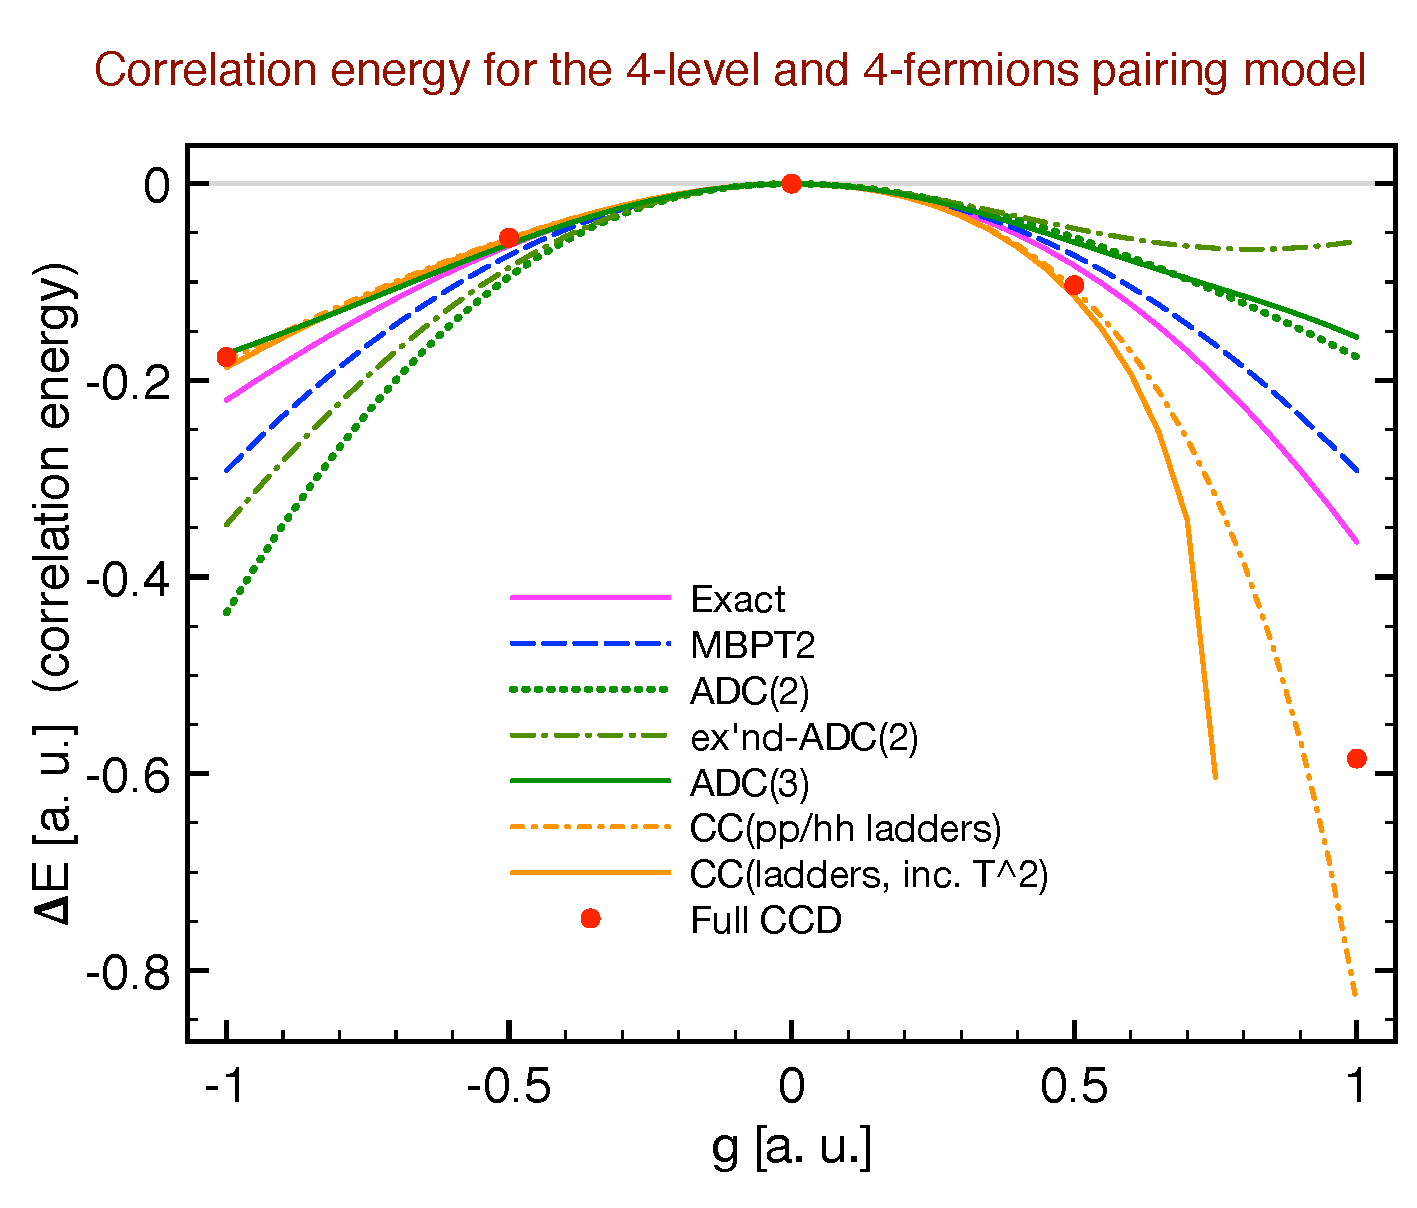
\includegraphics[width=0.8\textwidth]{Chapter11-figures/Pairing_model_CI_ADC_CC.pdf}
\caption{Self-energy insertion diagram that appear at third order in the perturbative expansion, with two-nucleon interactions, when the reference propagators are not self-consistent.  With the inclusion of three-nucleon interactions other two contribution arise that originate from the diagram of Fig.~\ref{fig:2ndOrd}b).  If a Hartree-Fock reference state is used these contributions cancel out (see {\bf Exercise 11.4}). }
\label{fig:SEins_3ndOrd}
\end{center}
\end{figure}


 
 
\subsection{Solving the Dyson equation}

 Once we have obtained and  appropriate approximation to the self-energy, it is necessary to solve the Dyson equations~\eqref{eq:Dyson} in order
 to obtain the single particle propagator and the observables associated with its spectral function. The latter will also yield spectroscopic amplitudes and their spectroscopic factor for the addition and removal of a nucleon form the correlated state $|\Psi^A_0\rangle$.  In doing this, Eq.~\eqref{eq:Dyson} takes the form of a one-body Schr\"odinger equation for the scattering of particle or holes states inside the medium. Given that all the Cauchy integrals associated with Feynman diagrams have been carries out, we can safely take the limit $\pm i \eta \rightarrow 0$ in all denominators, so that the same equation applies to states both above and below the Fermi surface. 
 Thus, it is convenient to take a general index $i$ and using $\varepsilon_i$ and $\pazocal Z^i$ to label energies and spectroscopic amplitudes for all quasiparticle and quasihole states. Specifically,
 \begin{equation}
\varepsilon_i \longrightarrow \left\{
\begin{array}{lcl}
\varepsilon_n^+ & \quad & \hbox{for $i$=$n$, particle,}  \\ ~ \\
\varepsilon_k^- &  & \hbox{for $i$=$k$ hole,} 
\end{array} \right.
\qquad \hbox{and} \qquad 
\pazocal Z^i_\alpha  \longrightarrow \left\{
\begin{array}{lcl}
\pazocal X^n_\alpha & \quad & \hbox{for $i$=$n$, particle,} \\ ~ \\
\pazocal Y^k_\alpha &  & \hbox{for $i$=$k$, hole.} 
\end{array} \right.
\label{eq:Z_ampl}
\end{equation}

In order to extract the solution for the pole $i$ in the Lehman representation, we extract the corresponding residue on both the left and right have sides of Eq.~\eqref{eq:Dyson}:
 \begin{equation}
   \lim _{\omega \rightarrow \varepsilon_i} 
   \left\{
     g(\omega) = g^{(0)}(\omega) + g^{(0)}(\omega)  \Sigma(\omega) g(\omega)
   \right\} \; ,
 \end{equation}
which gives 
 \begin{equation}
    \pazocal Z^i_\alpha (\pazocal Z^i_\beta)^*  =  \left. g^{(0)}(\omega)  \Sigma(\omega) \pazocal Z^i_\delta (\pazocal Z^i_\beta)^* 
    \right|_{\omega = \varepsilon_i}
 \; .
 \end{equation}
By dividing out $\pazocal Z^i_\beta$ and using the fact that $[g^{(0)}(\omega)]^-1 = \omega - (T + h_0)$ we finally obtain the 
eigenvalue equation
 \begin{eqnarray}
   \varepsilon_i   \pazocal Z^i_\alpha &=&   \left. \left\{ T +   \Sigma(\omega)   \right\}_{\alpha \, \delta}
  \pazocal Z^i_\delta  \right|_{\omega = \varepsilon_i}
  \nonumber \\
  &=&  \left. \left\{  T +  \Sigma^{(\infty)} +M^\dagger\frac1{\omega - E -C + i \eta}M +N\frac1{\omega - E -D - i \eta}N^\dagger     \right\}_{\alpha \, \delta}
  \pazocal Z^i_\delta  \right|_{\omega = \varepsilon_i}  \; ,
\label{eq:DysSchrod}
 \end{eqnarray}
where the potential $h_0$ defining the reference state completely cancels out and the irreducible self-energy $\Sigma(\omega)$
acts as a non-local and energy dependent potential that accounts for the motion both particle and holes inside the system, including 
coupling excitations.
At positive energies ($\omega > 0$) this equation describes the elastic scattering of a nucleon off the $|\Psi^A_0\rangle$ ground
states and the self-energy can be identified with a fully microscopic optical potential~\cite{Cederbaum2001,Capuzzi1996,Barbieri2005}.
In this case the spectroscopic amplitudes $\pazocal Z^i$ correspond to scattering wave function with corresponding asymptotic 
normalisation.
Instead, at $\omega < 0$ the Eq~\ref{eq:DysShrod}  describe the transition to states of $|\Psi^{A\pm1}_i\rangle$ with bound amplitudes. 
The norm of each $\pazocal Z^i$ gives the corresponding spectroscopic factor and it is obtained as
\begin{equation}
 S^i = \sum_\alpha |\pazocal Z^i_\alpha|^2 =  \frac 1 {1 - (\tilde{\pazocal Z}^i_\beta)^* 
   \left. \frac{d \, \Sigma^\star_{\beta \gamma}(\omega)}{d \, \omega} \right|_{\omega = \varepsilon_i}
    \tilde{\pazocal Z}^i_\gamma}   \; ,
\label{eq:SFnorm1}
\end{equation}
where $\tilde{\pazocal Z}^i \equiv {\pazocal Z}^i / \sqrt{S^i}$ is the spectroscopic amplitude normalised to 1.

Equations~\eqref{eq:DysSchrod} and~\eqref{eq:SFnorm1} are the central equations of the Green's function formalism and show how the 
single-particle propagator is the solution of one-body equation in which the self-energy play the role of the actual potential seen by a nucleon or a
hole propagating inside the correlated system. The energy dependence on this potential and its non-locality are a consequence of the many-body
dynamics. Eq.~\eqref{eq:SFnorm1} also show that the reduction of spectral strength commonly observed in correlate systems arises from the dispersion
properties of the self-energy.

 In spite of its beauty, Eq.~\eqref{eq:DysSchrod} is also the worst starting point to solve the Dyson equation in a discretised finite basis. Unless one is interested in just a few solutions near the Fermi surface or the model space is extremely small, this approach will require high computational times due to the large amounts of diagonalizations required to extract the correct eigenvalues. The reason is that root-finding algorithms are needed to match the eigenvalues $\varepsilon_i$ with the argument of  $\Sigma^\star(\varepsilon_i)$ but simple searching algorithms may miss a large amount of solutions. The consequences of missing a large portion of spectral strength are that wrong results would be obtained for the ground state observables discussed in Sec.~\ref{sec:scgf_obs}. This can also deteriorate the self-consistency already at the level of the static self-energy, $\Sigma{(\infty)}=\tilde{U}$.  If Eq.~\eqref{eq:DysSchrod} must be used, it is possible to gather all the necessary solutions by starting from extremely fine energy meshes to be sure that all eigenvalues are bracketed first. However, this easily becomes suicidal in terms of the increase of computing time.
 %
We discuss here an different approach that is not affected by these problema and that will also give some further insight into the physics content of the Dyson equation.

First, for each solution of the Dyson equation we define two new vectors $\pazocal{W}^i$ and  $\pazocal{V}^i$ which live in the ISC space as follows:
\begin{eqnarray}
 \sum_{r'}  [\omega - E -C ]_{r,r'}  \, \pazocal{W}^i_{r'} &\equiv& M_{r,\delta}   Z^i_\delta  \; ,
 %\label{eq:defW} \\
 \nonumber \\
 \sum_{s'}  [\omega - E -D ]_{s,s'} \, \pazocal{V}^i_{s'} &\equiv& N^\dagger_{s,\delta}    Z^i_\delta \; ,
 \label{eq:defWV}
\end{eqnarray}
where we have let $i\eta\rightarrow 0$ as this is no longer needed in a finite an discretised basis. With these definitions, Eq.~\eqref{eq:DysSchrod}  is easily rearranged into a sigle eigenvalue problem of larger dimensions but where the correspongdin matrix is energy independent:
\begin{equation}
\left( \begin{array}{ccccc}
 \hat{T} + \Sigma^{(\infty)}  &~&   M^\dagger   &~&  N~  \\
&&\\
    M   &&  C  && \\
    &&\\
    N^\dagger    &&      &&  D
\end{array} \right)
\left( \begin{array}{c}
\pazocal{Z}^i \\ ~ \\ \pazocal{W}^i \\~ \\ \pazocal{V}^i
\end{array} \right)
=\left( \begin{array}{c}
  \pazocal{Z}^i \\ ~\\ \pazocal{W}^i \\~\\ \pazocal{V}^i
\end{array} \right)
  \varepsilon_i
\label{eq:DysMtx}
\end{equation}
and the normalization condition~\ref{eq:SFnorm1} becomes
\begin{equation}
\sum_\alpha  |\pazocal Z^i_\alpha|^2 + \sum_r  |\pazocal W^i_r|^2 + \sum_s  |\pazocal V^i_s|^2 = 1   \; .
\label{eq:SFnorm2}
\end{equation}

The advantage of Eq.~\eqref{eq:DysMtx} is that it linearises the Dyson equation and yields all solutions in one single diagonalization. Although the dimension of the Dyson equation is much larger than a one-body Schr\"odinger problem and that it requires substantial amount of storage, it typically provides the full spectral strength 100 times faster than using Eq.~\ref{eq:DysSchrod} directly. Furthermore, it is possible to reduce the dimensionality of the eigenvalue problem by projecting matrices $C$ and $D$ (separately!) onto smaller Lanczos/Krylov spaces~\cite{Schirmar9?,Som14a}. In this way one reduces the number of poles of $g(\omega)$ far away from the Fermi surface--that do not have direct physical meaning--but conserve the overall strength needed to compute ground state observables.

Eq.~\eqref{eq:DysMtx} also puts in evidence how the Dyson equation is very closely related to a configuration interaction (CI) approach. For solutions ($\varepsilon^+_n$,$\pazocal{X}^n$) in the single particle spectrum,  the eigenstates of $|\Psi^{A+1}_n\rangle$ are expanded in terms of 1p configurations (from the $\hat{T} + \Sigma^{(\infty)}$ sector) and 2p1h or larger configurations, which is evident from matrix $C$, see Eqs.~\eqref{eq:ADC2_MC}. However, additional 2h1p configurations are included through matrix $D$. This is in spirit very similar to how ground state correlations are included in the random phase approximation approach~\cite{RingSchuck} but the eigenstates will approach the exact solution as the approximation of the sel-energy is systematically improved. Likewise, the propagation of hole states that correspond to eigenstates eigenstates of $|\Psi^{A-1}_k\rangle$ are obtained in a CI fashion.
Eq.~\ref{eq:SFnorm2} is then the natural normalization condition for the CI expansion and shows that the spectroscopic amplitudes are the projection of more complex many-body wave functions on a single partile space.

\vskip .5 cm
{\bf Exercise 11.5}.  Perform a Taylor expansion o the propagator $g$ at zero-th order around a given pole $\varepsilon_i^\pm$. Then use this and the 
conjugate Dyson equation [second line in Eq.~\eqref{eq:Dyson}] to obtain the normalizarion of spectroscopic factors given in  Eq.~\eqref{eq:SFnorm1}.


\vskip .5 cm
{\bf Exercise 11.6}.  Based on the definition of vectors $W$ and $V$ in Eqs.~\ref{eq:defWV}, show the Eqs.~\eqref{eq:SFnorm1} and~\eqref{eq:SFnorm2} are equivalent.



\subsection{A simple pairing model}

\begin{figure}[ht]
\begin{center}
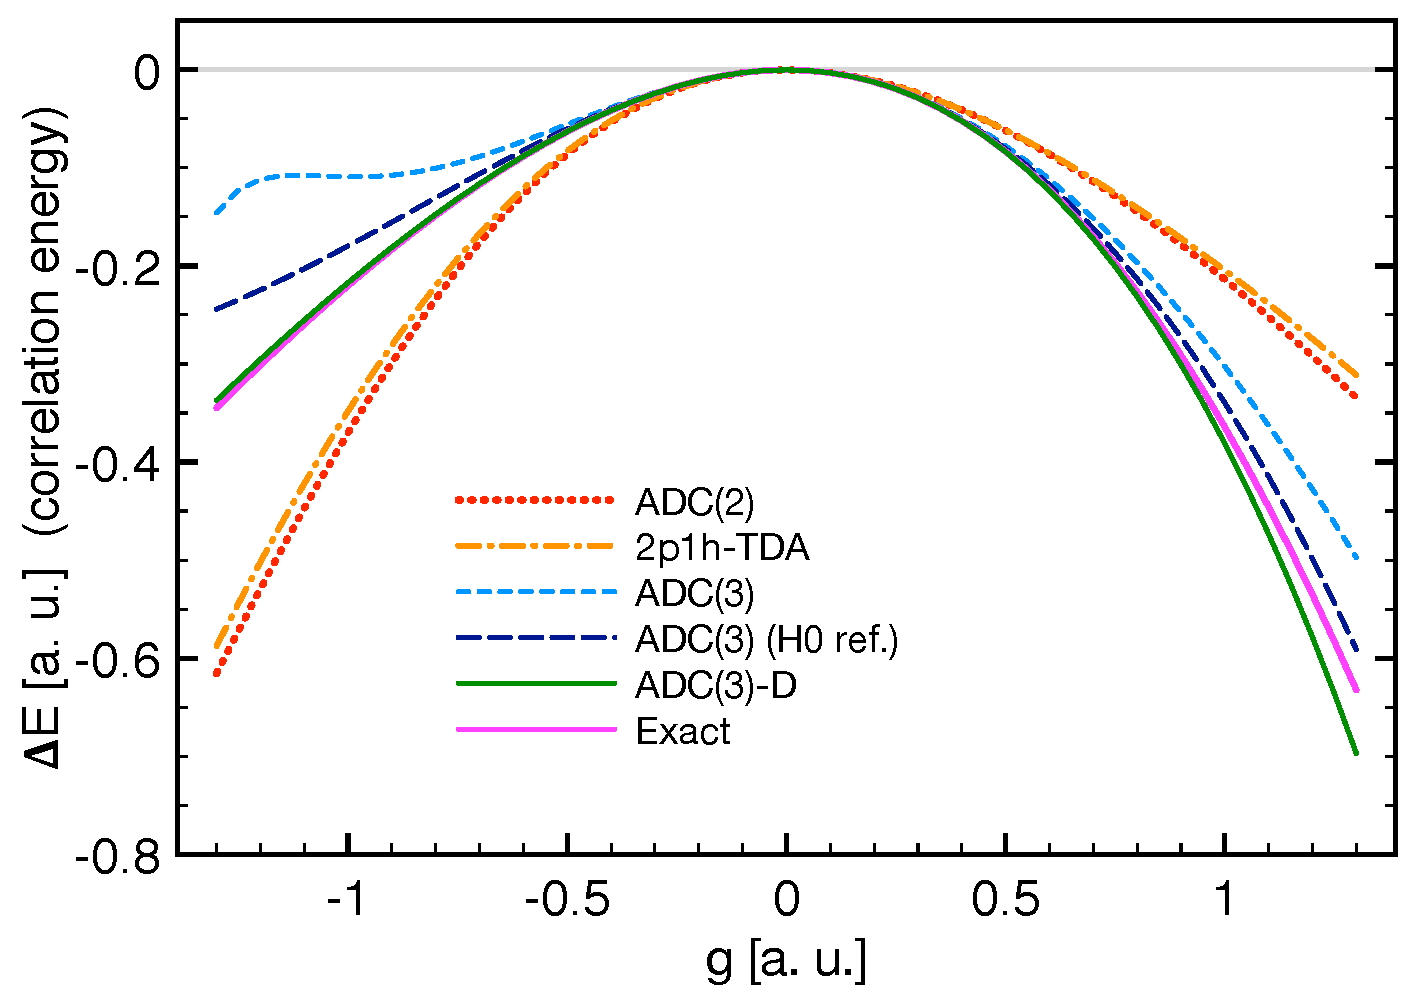
\includegraphics[width=0.8\textwidth]{Chapter11-figures/Pairing_LNP_scgf.pdf}
\caption{Correlation energy for the pairing Hamiltoninan of Eq.~\eqref{eq:H_pair} obtained for different  ADC(n) approximations
to the self-energy. The purple line shows the exact results from full CI theory. }
\label{fig:pairng_adc}
\end{center}
\end{figure}

\begin{figure}[ht]
\begin{center}
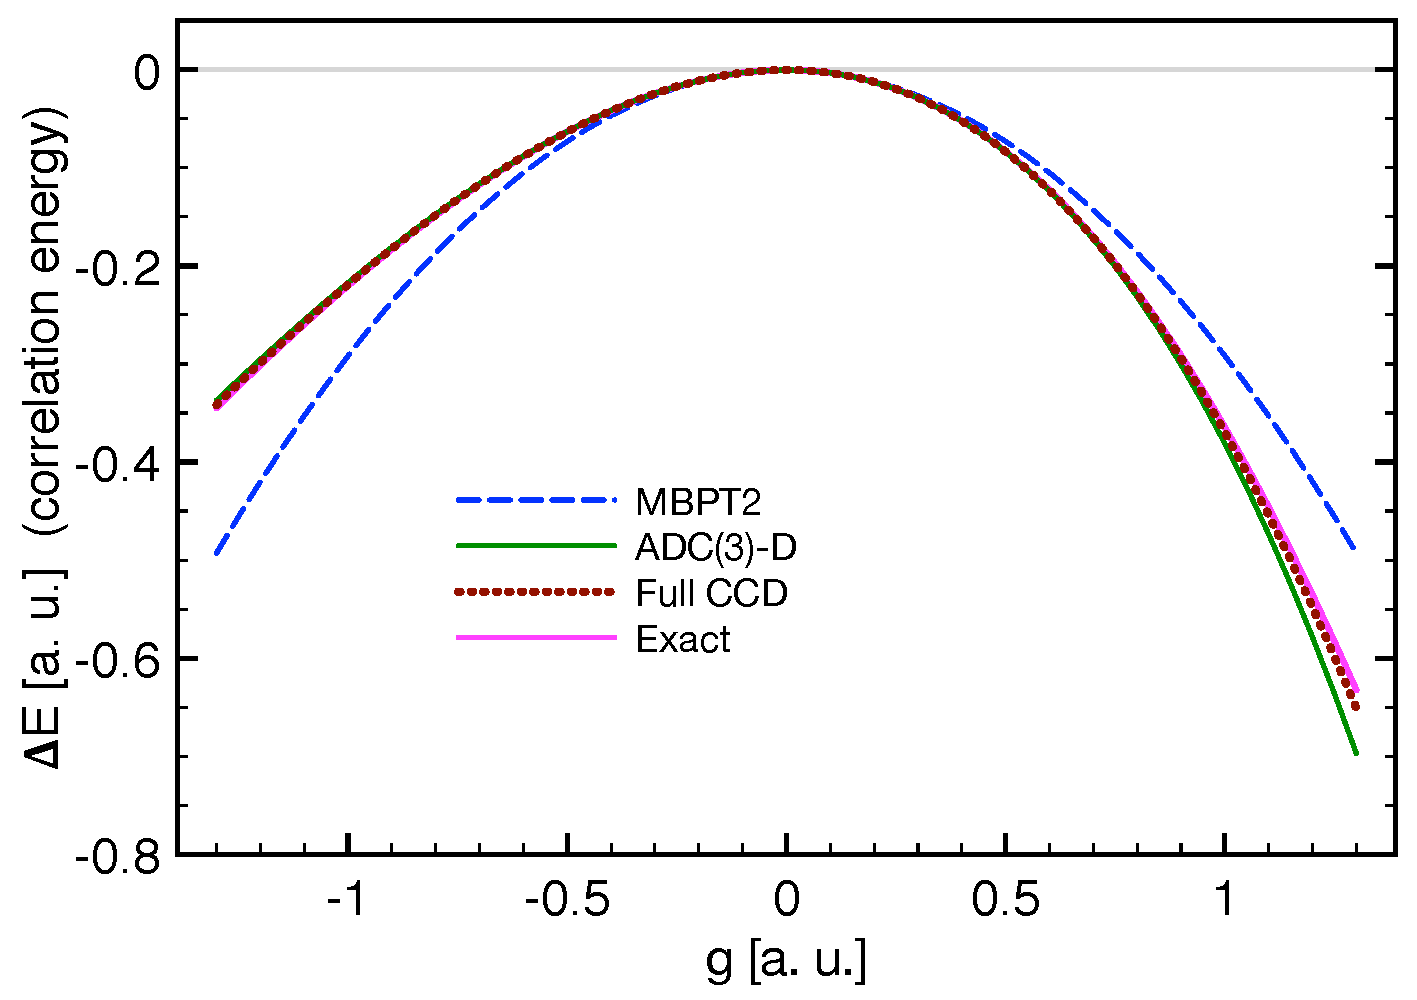
\includegraphics[width=0.8\textwidth]{Chapter11-figures/Pairing_LNP_ALL.pdf}
\caption{Correlation energy for the pairing Hamiltoninan of Eq.~\eqref{eq:H_pair} obtained for different
many-body methods. The purple line shows the exact results from full CI theory. Various CC approximations (as discussed in 
Chapter 8), the  second order perturbation theory (MBPT2)  and ADC(3) results are shown.}
\label{fig:pairng_all}
\end{center}
\end{figure}

As a first application of the ADC formalism, we consider here the paring Hamiltonian discussed in Chapter~\ref{chap:chapter8}. This is a system of  four spin-1/2 fermions in a 4-level model space that interact through a pairing force:
  \begin{equation}
   \hat{H} = \hat{H}_0 +  \hat{V} = \xi \sum_{p=1}^4  \sum{\sigma=+, -} (p-1) a^{\dagger}_{p \sigma} a_{p \sigma}
 ~-~ \frac{g}{2} \sum_{p, q=1}^4 a^{\dagger}_{p+}a^{\dagger}_{p-}  a_{q-}a_{q+}
\label{eq:H_pair}
\end{equation}


Note that the model of Eq.~\eqref{eq:H_pair} is a particularly difficult test for many-body approximation in which is does not conains
leading order contributions at the single particle level---hence CCS and 2p1h/2h1p contribution do not mix in the ground state---while 
higher configurations of 2p2h dominates (this is to be explained more clearly in the final draft). 


We perform calculations at different levels of approximation in the ADC(n) scheme. First, we implement the ADC(2) equations~\ref{eq:ADC2_MC} and~\ref{eq:ADC2_ND} and a hybrid scheme in which the matrices $M$ and $N$ remain the same as in ADC(2) but the use the third order  expressions 
for $C$ and $D$. The latter approximation in commonly referred to as 'extended-ADC(2)' and includes the all order summations of ladder and ring diagrams. However, it misses third order contributions to the coupling matrices that are important to obtain correct separation energies  for addition and removal of a particle.  The results for the correlations energy are compare to the exact FCI results in Fig.~\ref{fig:pairng_adc}, where it is seen that the extended-ADC(2)
gives a small improvement for a repulsive  interaction ($g<0$) but it deteriorated for attractive pairing.
The complete ADC(3) approximation corrects the issues of the extended-ADC(2) and becomes very close the the exact result for a repulsive pairing. However, for $g>0$, it does not improve upon the simple ADC(2).  This is mostly because of the lack of direct terms in Hamiltonian~\ref{eq:H_pair} that connect single particle states to 2p2h and 4p4h configurations...



A comparison with the CC approach (and other methods as well??) is presented in Fig.~\ref{fig:pairng_all}.
The ADC(3) and CCD methods perform similarly at $g<0$ where are both close to the exact solution. They deviate by similar amounts for attractive pairing but in opposite directions. {\color{blue} [RED DOTS  ARE THE NUMBER FOR FULL CCD  THAT GAUTE COMPUTED DURING TALENT IN JULY 2015. HOWEVER THEY DO NOT AGREE WTH WATH IS PRESENTED IN Fig.~8.4. THIS IS TO BE RESOLVED...]}

\section{A computational project in infinite matter}
\label{sec:scgf_comp}


In this section we discuss how to approach  ADC(3) calculations of infinite matter. We will do this 
using the C++ programming language and will refer to the numerical code provided with in this chapter.

the most important deciosnin in order to set up a SCGF calcualtion is the choice of the model space. For
infinite matter, trasnlational inviariance imposes that the Dyson equation is diagonal in momentum  and 
therefore it becomes much easier to solve the problem in momentum space. However, there remain two possible
choices for how to encode the single particle degrees of freedom. 
The first one is to subdivide the infiite space in  boxes of finite lenth  and to impose periodic bounduarry conditions
(see also Chapter 8). In this way, the number of fermions included in each box is finite and determined by the particle
density of the system. The resulting model space is naturally expressed by a set of discretised single particle 
states and equations in the form of Eqs.~\eqref{eq:ADC3_MC}, \eqref{eq:ADC3_ND} and \eqref{eq:DysMtx}
can be solve directly as ti would be done for a finte system in a box.  Numerical results then need to be converged 
with respect to the trunction of the k-space inside each box.   We will follow this approach for the present 
computational project.
The other approach is to retain the full momentum space and write the SCGF equations already in the full 
thermodynamic limit. This approach is more suitable to solve the Dyson equation in at finite temperatures and
in a full SCGF fashion and will be discussed furtes in Sections~\ref{sec:scgf_finiteT} and~\ref{sec:scgf_comp_finiteT}.


\vskip 0.5 cm
{\em Construction of the model space.}
\lstset{language=c++}
\begin{lstlisting}
    i_count = 0;
    for (int ix=-imax; ix<=imax; ++ix)
      for (int iy=-imax; iy<=imax; ++iy)
        for (int iz=-imax; iz<=imax; ++iz) {
          itest = ix*ix + iy*iy + iz*iz;
          if ((nsq_mn <= itest) && (itest <= nsq_mx)) ++i_count;
        }
\end{lstlisting}
Once we know how many single particle $\vec k$ states we have, we can allocate 
arrays in memory to store the relevant quantum numbers of each of them:
\begin{lstlisting}
  int i1 = this->Count_sp_basis(0, nsq_mx, imax);
 
  SpNAlloc = (ch_max - ch_min + 1) * 2 * i1 + 10; // +10 for safety
  
  cout << "\n allocating space for "<< SpNAlloc << " sp states... \n";
  
  nx    = new int[SpNAlloc];
  ny    = new int[SpNAlloc];
  nz    = new int[SpNAlloc];
  nsq   = new int[SpNAlloc];
  spin  = new int[SpNAlloc];
  chrg  = new int[SpNAlloc];
  k     = new double[SpNAlloc];
  e_kin = new double[SpNAlloc];
  e_HF  = new double[SpNAlloc];
  e_sp  = new double[SpNAlloc];
  group = new int[SpNAlloc];
  
  int ich, is;

  double xk = 0.0, xek = 0.0;
  
  i1 = 0;
  for (int isq=0; isq<=nsq_mx; ++isq) {
    for (int ix=-imax; ix<=imax; ++ix) {
      for (int iy=-imax; iy<=imax; ++iy) {
        for (int iz=-imax; iz<=imax; ++iz) {
          if ((ix*ix + iy*iy + iz*iz) != isq) continue;

          xek = double(isq);
          xk  = sqrt(xek) * 2.0 * PI / Lbox;
          xek = xk * xk * MeVfm * MeVfm / 2.0 / NUCLEONmass;  //nuc_mass_ave;
          cout << i1 << "  " << ix << "  " << iy << "  " << iz << "  ";
          cout << isq << "  " << xk << "  " << xek << endl;

          for (ich=ch_min; ich<=ch_max; ++ich)
            for (is=-1; is<2; is+=2) {
              nx[i1] = ix;
              ny[i1] = iy;
              nz[i1] = iz;
             nsq[i1] = isq;
            spin[i1] = is;
            chrg[i1] = ich;
               k[i1] = xk;
           e_kin[i1] = xek;
            e_HF[i1] = 0.0;
            e_sp[i1] = 0.0;
           group[i1] = -100;
            ++i1;
            }
        
        }
      }
    }
  }
  SpNmax = i1;
\end{lstlisting}

\vskip 0.5 cm
{\em Construction of ISCs.}

\vskip 0.5 cm
{\em Two body interaction: Minnesota potential}

\vskip 0.5 cm
{\em Hartree-fock theory}

\vskip 0.5 cm
{\em Constructing the Dyson matrix}

\vskip 0.5 cm
{\em Numerical solutions at ASDC(20 and ADC(3) level}



\begin{figure}[ht]
\begin{center}
%\includegraphics[width=0.8\textwidth]{Chapter11-figures/???}
\caption{Equation of state for pure neutron matter for the Minnesota interaction, as predicted by different ADC(n) approximations. ADC(2), extended-ADC(2) and the complete ADC(3) are shown.}
\label{fig:minn_adc_eos}
\end{center}
\end{figure}



\begin{figure}[ht]
\begin{center}
%\includegraphics[width=0.8\textwidth]{Chapter11-figures/???}
\caption{Spectral function of pure neutron matter at nomina saturation density ($\rho=0.16$~fm$^{-3}$) from ADC(3)---3D plot. }
\label{fig:minn_adc_sfnct}
\end{center}
\end{figure}


\section{Self-consistenft Green's functions at finite temperatures in the thermodynamic limit}
\label{sec:scgf_finiteT}

In the following we want to concentrate on the study of an infinite system at finite temperature; we will then set ourselves in the thermodynamic limit, i.e. number of particles $N$ and volume $V$ tending at infinity with density $\rho=N/V$ kept constant. The may-body SCGF approach at finite temperature is particularly suited for this kind of study because it is thermodynamically consistent, meaning that a quantity calculated from the microscopic point of view yields the same results as the thermodynamical macroscopic quantity~\cite{Baym1962}. This consistency is strictly related to the fact that a fully dressed propagator, obtained via iterative solution of Dyson's equation, is used in the calculation of the partition function in the Luttinger-Ward formalism~\cite{Luttinger1960}, to obtain the thermodynamical properties of the system. Furthermore, it can be demonstrated that this method fulfils the Hugenholtz van-Hove theorem~\cite{Hugenholtz1958}, and this once again relates to the fact that the conservation laws of particle number, momentum and energy are preserved in this kind of approximation~\cite{Baym1961,Baym1962}.

We will show how to calculate the self-consistent propagator in the ladder approximation, where particle-particle and hole-hole intermediate scattering states are resummed in the in-medium T-matrix, and then use the Koltun sumrule to obtain the total energy of the many-body system. Via the Luttinger-Ward formalism, the entropy can be calculated via the knowledge of the self-consistent propagator, and from the entropy all other thermodynamical quantities are accessible. We will first give a few hints on the theoretical formalism and then sketch the working equations necessary to perform the numerical calculation in the following section. The full self-consistent numerical calculation considering the complete off-shell properties of the system and considering fully microscopic potentials was performed by the T\"ubingen/Barcelona group~\cite{Frick2003,Frick2005,Rios2006C74,Rios2008,Rios2009} and from the Cracow group~\cite{Soma2006,Soma2008,Soma2009}.

We start by defining the one-body Green's function as a statistical average in the grand-canonical ensemble:
\begin{equation}
\label{thermalG}
iG({\bf x}t, {\bf x'}t')= {\rm Tr}\{\hat{\rho}{\pazocal T}[\hat\psi({\bf x}t) \hat\psi^\dagger({\bf x'}t')]\}\,,
\end{equation}
where ${\pazocal T}$ describes the Wick time-ordered product of the quantum field operators of creation and destruction of a SP state, $\hat\psi^\dagger({\bf x'}t')$ and $\hat\psi({\bf x}t)$ respectively. The field operators are related to the operators of creation and destruction, i.e. $c^\dagger_k$ and $c_k$, via $\hat\psi^\dagger({\bf x'}t')=\sum_k\psi({\bf x}t)^\dagger c^\dagger_k$ and $\hat\psi({\bf x}t)=\sum_k\psi({\bf x}t)c_k$, where the coefficients are the single-particle wave functions and the sum is over the complete set of single-particle quantum numbers. For simplicity the variable ${\bf x}$ defines altogether the position, spin and isospin quantum numbers of a SP state, so an integration over ${\bf x}$ implies an integration over the position ${\bf x}$ and a summation over spin/isospin numbers. The statistical factor $\hat \rho$ is defined by:
\begin{equation}
\hat \rho=\frac{1}{Z}e^{-\beta(\hat H -\mu\hat N)}\,,
\end{equation}
where $\beta=1/T$, and $Z$ is the grand-partition function
\begin{equation}
Z={\rm Tr}\,e^{-\beta(\hat H -\mu\hat N)}\,,
\end{equation}
with $\hat H$ and $\hat N$ the hamiltonian and the particle number operators respectively. The trace in Eq.~(\ref{thermalG}) is to be taken over a full set of energy and particle number eigenstates of the system. The two possible time-ordering products in Eq.~(\ref{thermalG}) are given by:
\begin{equation}
\label{Tproduct}
{\pazocal T}[\hat\psi({\bf x}t) \hat\psi^\dagger({\bf x'}t')]=
 \Bigg\{
  \begin{tabular}{c}
  \,\,\,\,$\hat\psi({\bf x}t) \hat\psi^\dagger({\bf x'}t'), \quad t>t'$  \\
  $-\hat\psi^\dagger({\bf x'}t') \hat\psi({\bf x}t), \quad t'>t$
  \end{tabular}
\end{equation}
The first time-ordered product in Eq.~(\ref{Tproduct}) describes the creation of a particle state at time $t'$ with quantum numbers ${\bf x'}$, and the destruction of the propagated particle state at time $t$ with quantum numbers ${\bf x}$. Analogously, the second time-ordered product in Eq~(\ref{Tproduct}) describes the destruction of a particle state, or creation of a hole state, at time $t$ with quantum numbers ${\bf x}$, and the creation of the propagated hole state at time $t'$ with quantum numbers ${\bf x'}$. From Eq.~(\ref{Tproduct}) one can define the correlation functions: 
\begin{eqnarray}
\label{corr_creat}
iG^>({\bf x}t, {\bf x'}t')&=& ~ ~ {\rm Tr}\{\hat{\rho}[\hat\psi({\bf x}t) \hat\psi^\dagger({\bf x'}t')]\} \\
iG^<({\bf x}t, {\bf x'}t')&=& -{\rm Tr}\{\hat{\rho}[\hat\psi^\dagger({\bf x'}t')\hat\psi({\bf x}t)]\}\,.
\label{corr_destr}
\end{eqnarray}
Depending on the specific time ordering, the Green's function defined in Eq.~(\ref{thermalG}) corresponds to one correlation function or the other. It is also useful to define the retarded propagator. This is that part of the one-body Green's functions which is related only to the causal  propagation of events, i.e. forward in time:
\begin{equation}
\label{retar_prop}
G^R({\bf x}t, {\bf x'}t')=\theta(t-t')[G^>({\bf x}t, {\bf x'}t')-G^<({\bf x}t, {\bf x'}t')]\,.
\end{equation}

If we look at the quantum field operators of creation and destruction defined in the Heisenberg picture
\begin{equation}
\label{atemp}
\hat\psi({\bf x}t)=e^{i\hat Ht}\hat\psi^\dagger({\bf x}0)e^{-i\hat Ht}\,
\end{equation}
it is then possible to observe a resemblance between the thermal weight factor $e^{\beta\hat H}$ and the time evolution operator $e^{i\hat Ht}$ when considering the imaginary time domain $t=-i\beta$. If one includes the expression (\ref{atemp}) in the definition of the correlation functions Eqs.(\ref{corr_creat}) and (\ref{corr_destr}), it can then be checked that for a certain imaginary time domain there is absolute convergence of the two expressions, specifically in the intervals $-i\beta<t-t'<0$ for $G^>$ and $0<t-t'<i\beta$ for $G^<$. Furthermore, it can be shown that the two correlation functions are related to one another at one of their imaginary time boundaries, providing the important relation: 
\begin{equation}
\label{qprelation}
G^<({\bf x},t=0;{\bf x'}, t')=e^{\beta\mu}G^>({\bf x},t=-i\beta;{\bf x'},t')\,.
\end{equation}
Thanks to the translational invariance under space and time of an infinite system, the Green's function only depends on the differences ${\bf r}={\bf x'}-{\bf x}$ and $\tau=t-t'$. Exploiting the quasi-periodicity relation of the Green's function along the imaginary time axis given in Eq.~(\ref{qprelation}), one can write a discrete Fourier representation in the frequency domain:
\begin{equation}
G({\bf r},\tau)=\int \frac{{\rm d}^3p}{(2\pi)^3}e^{i{\bf p}{\bf r}}\frac{1}{-i\beta}\sum_\nu e^{-iz_\nu\tau}G({\bf p},z_\nu)\,,
\end{equation}
where $z_\nu=\frac{\pi\nu}{-i\beta}+\mu$ are the Matsubara frequencies. The Fourier coefficients are then given by the inverse transformation:
\begin{equation}
\label{Fouriercoeff}
G({\bf p},z_\nu)=\int {\rm d}^3r\int_0^{-i\beta}{\rm d}\tau\,e^{-i{\bf p}{\bf r}+iz_\nu\tau}G({\bf r},\tau)\,.
\end{equation}
These coefficients are evaluated for an infinite set of complex frequencies, corresponding to the imaginary time domain, however one would like to understand the properties of the physical propagator, i.e. in the real time and frequencies domain. To do so let's go back to the expressions of the correlation functions and write down their Fourier transform:
\begin{eqnarray}
\label{FTpart}
G^>({\bf p},\omega) &=& i\int{\rm d}^3r\int_{-\infty}^{+\infty}{\rm d}\tau\,e^{-i{\bf pr}+i\omega t}G^>({\bf r},\tau)\,,\\
\label{FThole}
G^<({\bf p},\omega) &=& -i\int{\rm d}^3r\int_{-\infty}^{+\infty}{\rm d}\tau\,e^{-i{\bf pr}+i\omega t}G^<({\bf r},\tau)\,.
\end{eqnarray}
These two quantities now define the spectral probability to attach or remove a particle with an energy $\omega$ from the momentum state {\bf p} of the many-body system (we now omit for simplicity the spin/isospin quantum numbers). The sum of these two functions defines a positive quantity which we call the spectral function:
\begin{equation}
\label{spec_fun}
A({\bf p},\omega)=G^>({\bf p},\omega)+G^<({\bf p},\omega)\,.
\end{equation}
An important feature of the spectral function is that it fulfils the sumrule
\begin{equation}
\int_{-\infty}^{+\infty}\frac{{\rm d}\omega}{2\pi}A({\bf p},\omega)=1\,,
\end{equation} 
this is also a reason why one can speak about probabilities when referring to the spectral function. 

Inserting Eqs.(\ref{FTpart}) and (\ref{FThole}) in Eq.~(\ref{qprelation}), we can write the Fourier transform of the periodicity condition
\begin{equation}
G^>({\bf p},\omega)=e^{\beta(\omega-\mu)}G^<({\bf p},\omega)\,,
\end{equation}
and considering the definition of the spectral function, we can write the correlation functions in momentum/frequency:
\begin{eqnarray}
\label{FTpart}
G^<({\bf p},\omega) &=& f(\omega)A({\bf p},\omega)\,,\\
\label{FThole}
G^<({\bf p},\omega) &=&[1-f(\omega)]A({\bf p},\omega)\,,
\end{eqnarray}
where $f(\omega)=\frac{1}{1+e^{\beta(\mu-\omega)}}$ is the Fermi-Dirac distribution function. These expression show that once the spectral function is known it is easy to access the correlation functions. It is then also possible to write a similar expression for the Fourier coefficients defined in Eq.(\ref{Fouriercoeff}):
 \begin{equation}
\label{FT_fullprop}
G({\bf p},z_\nu)=\int^{+\infty}_{-\infty} \frac{{\rm d}\omega'}{2\pi} \frac{A({\bf p},\omega')}{z_\nu-\omega'}\,.
\end{equation}
The previous expression is performed for an infinite set of frequencies in the imaginary time domain. However one would like to extend this to the entire complex plane, especially close to the real-time domain. It can be demonstrated that this analytical continuation is possible and one can safely replace $z_\nu=z$. [Baym61]. This property that relates the Green's function $G({\bf p},z)$ in the complex plane to the spectral function $A({\bf p},\omega)$ is called the spectral decomposition of the single-particle propagator. A similar Fourier transform can be written for the retarded propagator defined in Eq.~(\ref{retar_prop}):
 \begin{equation}
\label{FT_retarprop}
G^R({\bf p},\omega)=\int^{+\infty}_{-\infty} \frac{{\rm d}\omega'}{2\pi} \frac{A({\bf p},\omega')}{\omega_+-\omega'}\,,
\end{equation}
with $\omega_+=\omega+i\eta$. At this point, exploiting the Plemelj identity,
\begin{equation}
\frac{1}{\omega\pm i\eta}=\frac{\pazocal P}{\omega}\mp i\pi\delta(\omega)\,,
\end{equation}
one can separate the real and imaginary part of the retarded propagator, and it can be checked that the imaginary part of the retarded propagator coincides with the spectral function up to a factor:
\begin{equation}
\label{spec_img}
A({\bf p},\omega)=-2{\rm Im}G({\bf p},\omega_+)\,.
\end{equation}
By introducing the algebraic form of Dyson's equation:
\begin{equation}
G({\bf p},\omega_+)=\frac{1}{[G_0({\bf p},\omega_+)]^{-1}-\Sigma^\star({\bf p},\omega_+)}\,,
\label{G_algebraic}
\end{equation}
into Eq.~(\ref{spec_img})
one can express the spectral function as:
\begin{equation}
A({\bf p},\omega)=\frac{-2\mathrm{Im}\Sigma^\star({\bf p},\omega_+)}
{[\omega-\frac{p^2}{2m}-\mathrm{Re}\Sigma^\star({\bf p},\omega)]^2+[\rm{Im}\Sigma^\star({\bf p},\omega_+)]^2} \,.
\label{spectral_fun}
\end{equation}
The numerical self-consistent solution that one has to perform is the one given by Eq.~(\ref{spectral_fun}). This means that one performs an iterative calculation up to the point when the spectral function inserted in the calculation of the irreducible self-energy is equal to the one obtained by solving Eq.~(\ref{spectral_fun}).

Before going on, it is interesting to see that in the limit of zero temperature, the spectral decomposition of the one-body propagator given in Eq.~(\ref{FT_fullprop}) can be written as:
\begin{equation}
G({\bf p},\omega)=\int_{\varepsilon_\textrm F}^\infty\mathrm d\omega'\frac{S^p({\bf p},\omega')}{\omega-\omega'+i\eta}
+\int_{-\infty}^{\varepsilon_\textrm F}\mathrm d\omega'\frac{S^h({\bf p},\omega')}{\omega-\omega'-i\eta}\,,
\label{Lehm_infty}
\end{equation}
The $S^p({\bf p},\omega)$ and $S^h({\bf p},\omega)$ correspond to the particle and hole spectral functions respectively. Notice that we have now introduced one single Fermi energy $\varepsilon_\textrm F$ ($\varepsilon_\textrm F$ = $\varepsilon_\textrm F^+$ = $\varepsilon_\textrm F^-$) which, in an uncorrelated system, defines the last filled energy level and hence corresponds to the energy needed to remove a particle from the many-body ground state. In the case of an interacting system, not in the superfluid nor in the superconducting phase, $\varepsilon_\textrm F$ equals the chemical potential $\mu$, and corresponds to the minimum energy necessary to add or remove a particle to/from the many-body system. Consequently, the expression for the spectral function given in Eq.~(\ref{spectral_fun}) can be divided into two parts:
\begin{eqnarray}
S^p({\bf p},\omega)&=&-\frac{1}{\pi}\frac{\mathrm{Im}\Sigma^\star({\bf p},\omega)}
{(\omega-\frac{p^2}{2m}-\mathrm{Re}\Sigma^\star({\bf p},\omega))^2+(\rm{Im}\Sigma^\star({\bf p},\omega))^2} \quad \omega>\varepsilon_\textrm F\,,\qquad\,\,\,
\label{Sp_self}
\\ 
S^h({\bf p},\omega)&=&\frac{1}{\pi}\frac{\mathrm{Im}\Sigma^\star({\bf p},\omega)}
{(\omega-\frac{p^2}{2m}-\mathrm{Re}\Sigma^\star({\bf p},\omega))^2+(\rm{Im}\Sigma^\star({\bf p},\omega))^2} \quad\,\,\,\, \omega<\varepsilon_\textrm F\,.\quad
\label{Sh_self}
\end{eqnarray}

In the next subsection we will briefly sketch the steps that have to be taken to perform the numerical implementation of Eq.~(\ref{spectral_fun}) at finite temperature.

\subsection{Numerical implementation at finite temperature}
We show in Fig.~\ref{num_impl} a schematic representation of how the code works when considering both two-body and three-body forces. %Depending on the starting point of the iteration procedure, $\sim15$ iterations are needed to obtain converged results. These could be less for low densities and high temperatures, and if the starting point is a converged iteration for another density, temperature state of the system. The number of iterations for convergence increase for lower temperatures and high densities. 
The fundamental quantities that one has to calculate are the first-order two-body Green's function, the in-medium $T$-matrix and the irreducible self-energy, which are depicted in the the three blue boxes in Fig.~\ref{num_impl} with their respective Feynman diagrams. Following Feynman rules, diagrams are a direct way to write down the mathematical expressions that one has to solve numerically. For clarity, we will distinguish between the wording \emph{calculation} and \emph{iteration}: we will refer to \emph{calculation} as the set of several \emph{iterations} necessary to get to a converged results for the spectral function, so an \emph{iteration} is exactly what is depicted in Fig.~~\ref{num_impl}. For a more in depth explanation of the numerical details the reader can refer to [Frickthesis,Riosthesis].

 
\begin{figure}[t]
\begin{center}
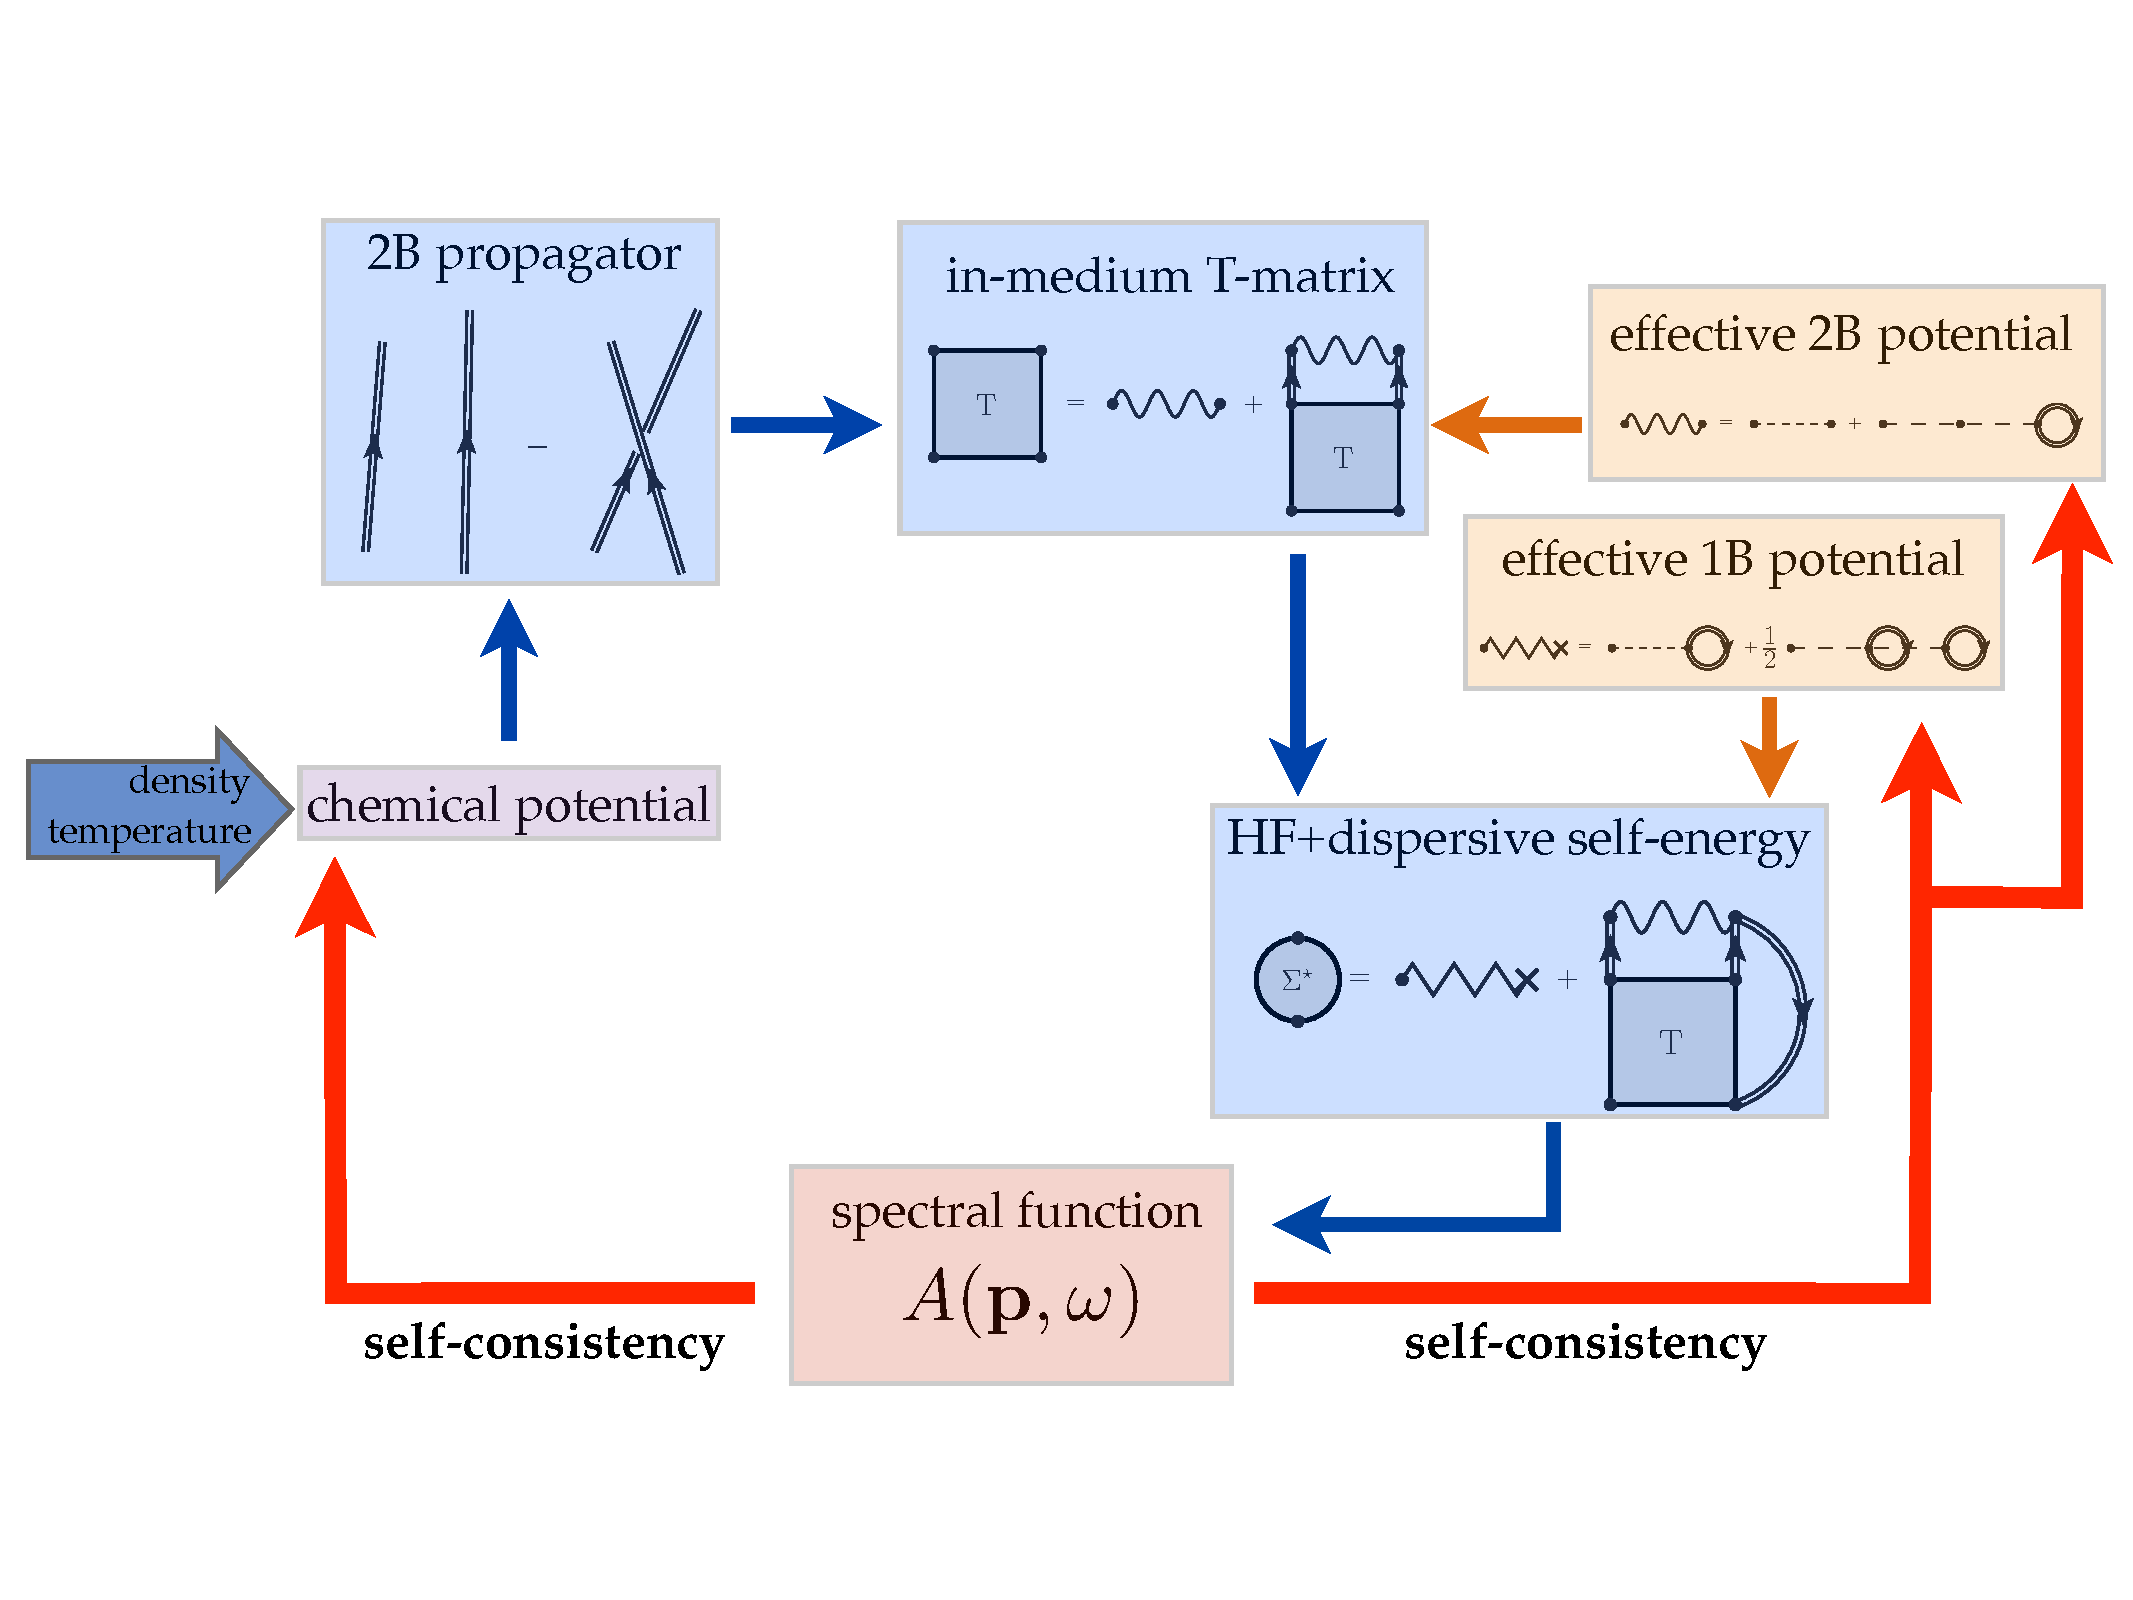
\includegraphics[width=1.0\textwidth]{Chapter11-figures/numerical_scgf_diagrams.pdf}
\caption{The structure of a ladder SCGF calculation including both two-body and three-body forces. Each quantity is also represented via a Feynman diagram.}
\label{num_impl}
\end{center}
\end{figure}


One starts the calculation from the thick external left arrow in Fig.~\ref{num_impl}, which corresponds to the input quantities: the density $\rho$ and temperature $T$ of the system. These, together with the imaginary, Im$\Sigma^*({\bf p},\omega)$, and real part, Re$\Sigma^*({\bf p},\omega)$, of the irreducible self-energy and the single-particle spectrum $\varepsilon({\bf p})$ obtained from a previous converged calculation are the ingredients to start with. 
\begin{itemize}
\item {\bf Numerical tips:}
The mesh of the single-particle momentum ${\bf p}$ for the self-energy is adjusted during the first iteration to be more dense around the Fermi momentum $p_{\rm F}$ corresponding to the specific density considered: $N_{\bf p}=70$ mesh points are enough, considering linear meshes at low momentum and around the Fermi momentum, and a logarithmic mesh for the tail all the way up to a value $\sim10p_{\rm F}$. The mesh in the single-particle energy $\omega$ has to be very dense because of the complicated features of the spectral function, especially at the quasi-particle peak. However storing a dense mesh at each iteration is demanding in terms of memory; for this reason one saves separately the imaginary and real part in a sparse mesh, $N_{\omega}=~6000$ linear mesh points from [-2000:15000] MeV, and then interpolates these quantities during the iterations to a denser meshes, $N_{\omega}=~30000$ linear mesh points, in order to have a good description of the spectral function in the energy domain. However, as it will be explained later on, the mesh in energy is adjusted in different ways during the iteration according to the specific quantities that one has to calculate (two-body propagator, T-matrix, etc.).
\end{itemize}

\noindent {\bf 1.} The density, temperature, spectral function and single-particle spectrum are the inputs to calculate the first quantity: the chemical potential. This is done by considering the relation:
\begin{equation}
\rho=\nu\int\frac{{\rm d}{\bf p}}{2\pi^3}\int_{-\infty}^{+\infty}\frac{{\rm d}{\omega}}{2\pi}A({\bf p},\omega)f(\omega,\mu)\,.
\label{chempot_micro}
\end{equation}
\begin{itemize}
\item {\bf Numerical tips:} One chooses a mesh of chemical potentials to insert in the Fermi-Dirac function $f(\omega,\mu)$ and solves the equation to find the one that matches the value of the external density. The mesh can be initially distributed around the value of the single-particle spectrum calculated at $p_{\rm F}$ (in the case of a zero temperature calculation it holds the relation $\varepsilon(p_{\rm F})=\mu$), and then adjusted testing if the limits include the value of the external density. However, it must be noted that the $\varepsilon({\bf p})$ comes from a different calculation, as also the chemical potential which enters the spectral function, so its has to be kept in mind that in the solution of Eq.~(\ref{chempot_micro}) one is considering two different chemical potentials, which will end up coinciding at the end of the convergence loop.
\end{itemize}

\noindent {\bf 2.} From the chemical potential one solves a self-consistent equation in the energy to find a new single-particle spectrum:
\begin{equation}
\varepsilon({\bf p})=\frac{p^2}{2m}+{\rm Re}\Sigma({\bf p},\varepsilon({\bf p}))\,,
\end{equation}
this will be used throughout the iteration. 
 
\noindent{\bf 3.} At this point the imaginary part of the first-order two-body Green's function can be calculated. The first order approximation of the two-body propagator corresponds to the independent propagation of two fully dressed particles. This includes two terms, a direct and an exchange one, (as depicted diagrammatically in Fig.~\ref{num_impl}). The imaginary part of this quantity reads:
\begin{equation}
\label{gII_imag}
{\rm Im}G^{II,f}_{pphh}(\Omega_+;{\bf p},{\bf p'}) = -\frac{1}{2}\int_{-\infty}^{+\infty}\frac{{\rm d}{\omega}}{2\pi}A({\bf p},\omega)A({\bf p'},\Omega-\omega)[1-f(\omega)-f(\Omega-\omega)]\,.
\end{equation}
where $\Omega_+$ is the sum of the energies of the two particles considered close to the real axis. This expression is derived from a sum over Matsubara frecuencies of a function with a double pole on the real-energy axis via use of the Cauchy theorem.
\begin{itemize}
\item {\bf Numerical tips:} The integrand of Eq.~(\ref{gII_imag}) will be particularly hard to resolve in the energy range where the two spectral functions are peaked. It can be demonstrated that performing a convenient variable change, one is safe with defining a mesh in energy accurately distributed around two specific regions, e.g. $\tilde\omega=0$ and $\tilde\omega=\tilde\Omega$ [for details see Ref.[Riosthesis]]. To obtain the spectral function in this specific mesh one interpolates the imaginary and real self-energies to this mesh and then solves Eq.~(\ref{spectral_fun}).
\end{itemize}

\noindent{\bf 4.} From the imaginary part it is then possible to obtain the real-part of the first-order two-body Green's function via a dispersion relation:
\begin{equation}
{\rm Re}G^{II,f}_{pphh}(\Omega_+;{\bf p},{\bf p'}) = -{\pazocal P}\int_{-\infty}^{+\infty}\frac{{\rm d}{\Omega'}}{\pi}\frac{{\rm Im}G^0_{II}(\Omega_+;{\bf p},{\bf p'})}{\Omega-\Omega'}]\,.
\end{equation}

\noindent{\bf 5.} An angle average is then necessary to calculate $G^{II,f}$. This average is necessary to circumvent the coupling of partial waves with different total angular momentum $J$ which appear in $G^{II,f}$. The average is performed over the angle formed by the center of mass momentum ${\bf P}$ and the relative momentum of the two nucleons ${\bf k}$. This strategy will facilitate the solution of the Lippmann-Schwinger equation to evaluate the effective interaction in the medium, known as the T-matrix. The average reads:
\begin{equation}
\overline{G^{II,f}_{pp,hh}}(\Omega;{\bf P},{\bf k})=\frac{1}{2}\int_{-1}^{+1}{\rm d\,cos}\theta G^0_{II}(\Omega;|{\bf P}/2+{\bf k}|,|{\bf P}/2-{\bf k}|)\,.
\end{equation}

\noindent{\bf 6.} The two-body angle-averaged propagator together with the nuclear potential are used to obtain the in-medium T-matrix. As explained previously, this is a ladder resummation of particle-particle and hole-hole diagrams, this differs with respect to the Brueckner G-matrix presented in Chapter 8 because it includes hole-hole diagrams and considers the full off-shell description of the spectral function. As seen from Fig.~\ref{num_impl}, the potential to be included is the sum of a bare two-body potential and an averaged three-body one. Details on the numerical solution for the average are given in the next section, while working equations for 3N chiral forces will be given in Appendix 1. The Lippmann-Schwinger type equation to be solved reads:
\begin{equation}
\label{t-matrix}
\langle{\bf k'}|{\rm T}(\Omega_+,{\bf P})|{\bf k}\rangle=\langle{\bf k'}|V^{\rm 2N}+\tilde V^{\rm 3N}|{\bf k}\rangle+\int {\rm d}{\bf k_1}\langle{\bf k'}|V^{\rm 2N}+\tilde V^{\rm 3N}|{\bf k_1}\rangle\overline{G^{II,f}_{pp,hh}}(\Omega;{\bf P},{\bf k_1})\langle{\bf k_1}|{\rm T}(\Omega_+;{\bf P})|{\bf k}\rangle\,.
\end{equation}
This is a one dimensional integral equation for each allowed combination of $J,\,S,\,T$, and at most two coupled values of $L$, due to the tensor component of the nuclear interaction. By means of a discretization procedure, the equation for the $T$-matrix is converted into a complex matrix equation which can be solved via standard numerical techniques [Rios]. A matrix inversion has to be performed to solve this equation. This can be quite demanding if the dimension of the matrix is large. 
\begin{itemize}
\item {\bf Numerical tips:} It is important to sample in a correct manner the number of integration mesh points without loosing physical information. This is achieved by sampling conveniently the region where $G^{II,f}$ is maximum in the relative momentum, so for $\Omega>0$ close to the pole $k'=\sqrt{m\Omega}$, and the high relative momentum region where, due to correlations, $G^{II,f}$ might not be negligible. Furthermore there is a node for $\Omega=2\mu$ present in the $T$-matrix so an accurate mesh for the bosonic energies around this value is needed for the forthcoming calculation of the self-energy.
\end{itemize}
At low temperatures, the appearance of bound states signals the onset of the pairing instability. This would directly appear as a pole in the matrix which has to be inverted to solve the Lippmann-Schwinger equation, for ${\bf P}=0$ and $\Omega=2\mu$. However, this should be seen only below a critical temperature which is around $T_c\sim4$ MeV. The calculations should not go below this border line in temperature. Especially in the case of symmetric nuclear matter, convergence at this temperature and for increasing density starts to be slow and difficult to achieve. This is due to the neutron-proton pairing in the coupled $^3S_1-^3D_1$ channel. In pure neutron matter, where this channel is not available, convergence is good all the way up to high densities, even for low temperatures. 

\noindent{\bf 7.} The remaining step in the SCGF method is the calculation of the self-energy from the T-matrix. The first quantity to be obtained is the imaginary part of the self-energy, Im$\Sigma^\star$:
\begin{equation}
{\rm Im}\Sigma_L({\bf p},\omega_+)=\int\frac{{\rm d}{\bf p'}}{2\pi^3}\int_{-\infty}^{+\infty}\frac{{\rm d}{\omega'}}{2\pi}\langle{\bf pp'}|{\rm Im}{\rm T}(\omega+\omega'_+,{\bf P})|{\bf pp'}\rangle A({\bf p'},\omega')[f(\omega')+b(\omega+\omega')]\,;
\end{equation}
We recall that this expression is also obtained from a summation over Matsubara frequencies of a function with two poles on the real energy axis. 
\begin{itemize}
\item {\bf Numerical tips:} A momenta and energy integrals have to be performed, taking special care for the pole in energy of the Bose function $b(\Omega)$. This pole is canceled by the node we had previously mentioned in the T-matrix, for this reason we had already defined a convenient mesh for $\Omega$ around the node. 
\end{itemize}
 
\noindent{\bf 8}. The real part of the self-energy is then obtained by means of a dispersion relation from the imaginary part: 
\begin{equation}
{\rm Re}\Sigma_L({\bf p},\omega_+)=\Sigma_{HF}({\bf p})-{\pazocal P}\int_{-\infty}^{+\infty}\frac{{\rm d}{\lambda}}{\pi}\frac{{\rm Im}\Sigma_L({\bf p},\lambda_+)}{\omega-\lambda}\,.
\end{equation}
The HF part of the SP self-energy is then calculated directly from the potential and the single particle momentum distribution $n({\bf p})$:
\begin{equation}
\label{HF_self}
\Sigma_{HF}({\bf p})=\int\frac{{\rm d}{\bf p'}}{2\pi^3}n({\bf p'})\Big[\langle{\bf pp'}|V^{\rm 2N}|{\bf pp'}\rangle +\frac{1}{2}\langle{\bf pp'}|\tilde V^{\rm 3NF}|{\bf pp'}\rangle\Big] 
\end{equation}
To evaluate this quantity, the calculation of the momentum distribution $n({\bf p})$ is needed. Detailed description on how to calculate this quantity and numerical details are given in Sec. 1.5.3. 

Finally, via Eq.~(\ref{spectral_fun}) the spectral function can be obtained and the procedure starts again until a consistent result is achieved. According to the mesh points in which the spectral function is needed, the interpolation is done on the imaginary and real part of the self-energy, and not directly on the spectral function. This is done in order to avoid incorrect samplings of the structure of the spectral functions which could induce numerical inaccuracies. We must point out that the energy mesh for the evaluation of the spectral function must be accurate enough to reproduce not only the quasi-particle peak region, but furthermore the low and high-energy tails which characterize the spectral function.   

\subsection{Calculations of neutron matter at finite temperatures.}
\label{sec:scgf_comp_finiteT}

We show here the result form pure neutron matter calculated with the Minnesota interactions. Fig.~\ref{fig:minn_SE} shows the self-energy at temperature
T=10~MeV and at momentum $k=2 K_F/3$  for nominal saturation density...  [ALL RESULTS TO BE DECIDED AND INCLUDED].

\begin{figure}[ht]
\begin{center}
%\includegraphics[width=0.8\textwidth]{Chapter11-figures/???}
\caption{Self-energy for pure neutron matter??? }
\label{fig:minn_SE}
\end{center}
\end{figure}


We finally compare results for different methods discussed in this book in Fig.~\ref{fig:minn_all}...

\begin{figure}[ht]
\begin{center}
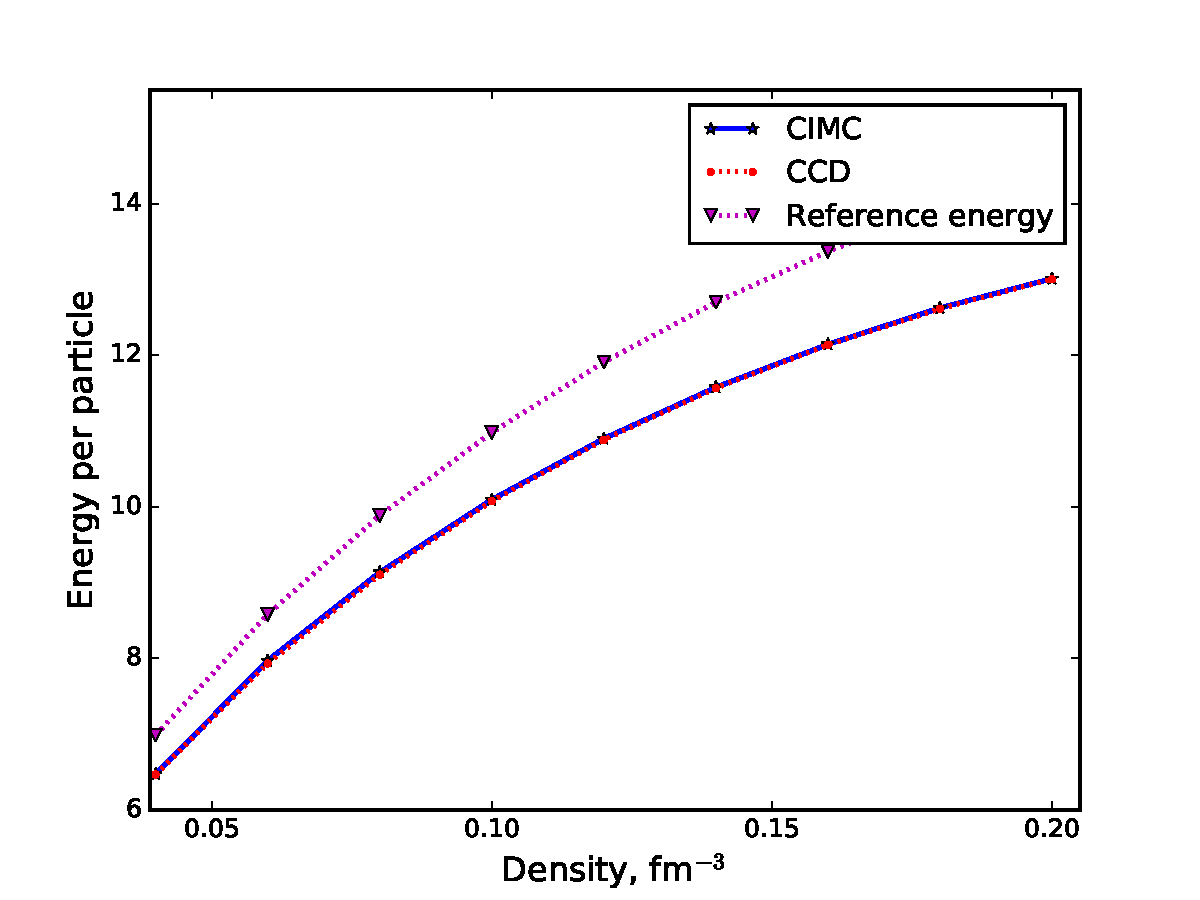
\includegraphics[width=0.8\textwidth]{Chapter11-figures/cimcccd.pdf}
\caption{Equation of state for pure nuclear matter obtained from different methods presented in this book. This would include CCD, IM-SRG and ADC(3) in 
a discretised cartesian basis,  AFDMC calculations, and full pp-hh resummation in SCGF at finite temperature (extrapolated to T=0).}
\label{fig:minn_all}
\end{center}
\end{figure}




\subsection{Numerical calculation when including three-body forces.}
As shown in Fig.~\ref{num_impl}, the inclusion of a one-body averaged 3N forces enters the calculation, as it is also explicitly shown in Eqs.~(\ref{t-matrix}) and (\ref{HF_self}). This average corresponds to a trace over the spin/isospin quantum numbers of the averaged particle, in this case the third particle, and by an integration over its momentum:
\begin{equation}
%\nn &&
\langle {\bf p'_1 p'_2}|\tilde V^\mathrm{3NF}|{\bf p_1 p_2}\rangle_A =
\mathrm{Tr}_{\sigma_3}\mathrm{Tr}_{\tau_3}
\int \frac{{\mathrm d}{\bf p}_3}{(2\pi)^3}n({\bf p}_3)
%\\ && \quad\quad\quad\quad\quad
\langle {\bf p_1' p_2' p_3}|V^\mathrm{3NF}
(1-P_{13}-P_{23})
|{\bf p_1 p_2 p_3}\rangle_{A_{12}}\ \,,
\label{dd3bf_new}
\end{equation}
where we have omitted the spin/isospin indices in the potential matrix elements for a better view. In Eq.~\ref{dd3bf_new} the ket on the right hand side is antisymmetrized only with respect to particles 1 and 2, i.e. ${\rm A}_{12}=(1-{\rm P}_{12})/2$, part which is not affected by the averaging procedure over particle 3; ${\rm P}_{12}=(1+\boldsymbol \sigma_1\cdot\boldsymbol \sigma_2)(1+\boldsymbol \tau_1\cdot\boldsymbol \tau_2)/4$ is the permutation operator of momentum and spin/isospin quantum numbers of particles 1 and 2. The momentum distribution that appears in Eq.~(\ref{dd3bf_new}) can be obtained directly from the spectral function, via the relation:
\begin{equation}
\label{mom_dist}
n({\bf p})=\int_{-\infty}^{+\infty}\frac{{\rm d}\omega}{2\pi}A({\bf p},\omega)f(\omega)
\end{equation}

Let us give some details on the numerical implementation for the calculation of Eq.~\ref{dd3bf_new} regarding the mesh of the internal momentum ${\bf p_3}$ and the calculation of the momentum distribution $n({\bf p_3})$ via Eq.~\ref{mom_dist}:
\begin{itemize}
\item We start with the definition of the mesh necessary to calculate the integral over the internal momenta ${\bf p}_3$. Considering that in the inegral we deal with a dressed distribution function $n({\bf p}_3)$, which may have populated states at high momentum, we need to cover momenta up to a certain high value in which it is sure that the $n({\bf p}_3)$ has reached zero. We define three Gauss-Legendre meshes respectively from $0$ to $p_\textrm F/3$, from $p_\textrm F/3$ to $p_\textrm F+p_\textrm F/3$, from $p_\textrm F+p_\textrm F/3$ to $3p_\textrm F$. Meshes are chosen to cover accurately the behavior of the distribution function from momenta lower to those higher than $p_\textrm F$. Finally, high momenta after $p_\textrm F$ are represented through a tangential mesh. We have 100  points in the Gauss-Legendre meshes, and 100 in the tangential one. 
\item We then need to calculate the momentum distribution function via solution of Eq.~(\ref{mom_dist}), so the spectral function coming from the previous iterative step has to be used. The values of the imaginary and real part of the self-energy are stored at each iterative step for different points in the energy and momentum space: for the momentum mesh we have $N_k=70$, for SP momenta going from 0 to 3000 MeV; for the energy mesh we interpolate through a spline the values of the imaginary and real part of the self-energy to a fine energy mesh of $N_{\omega,\textrm{spline}}=30000$ in a smaller range of values from [-2000:5000] MeV. These values are used to calculate the spectral function (see Eq.~(\ref{spectral_fun})) necessary to evaluate correctly Eq.~(\ref{mom_dist}). The integral in Eq.~(\ref{mom_dist}) is then performed via a trapezoidal integral in the energy range. Finally we perform a linear interpolation of the obtained values of $n({\bf p})$ to the mesh of ${\bf p}_3$ defined for the integration of the quantities in the density-dependent force. Extrapolated values are set to zero.
\end{itemize}

\noindent
Here we show a simple Fortran code to perform the previous two steps (gauss() is a common routine to perform a gauss-legendre mesh; splin() and splin2() are common routines to perform spline interpolations; linint() is a common routine to perform linear interpolation):

\vspace*{0.3cm}
\lstset{alsolanguage=[90]Fortran}
\begin{lstlisting}
    ! ... MOMENTA MESH FOR INTEGRALS OVER MOMENTUM DISTRIBUTION 

    write(*,*) "Correlated distribution function for averaged 3BF integration"

    Nk1=100
    Nk2=100
    Nk3=3d0*Nk1+Nk2
    ALLOCATE(xk3(Nk3),wk3(Nk3))
    ALLOCATE(xaux(Nk2),waux(Nk2))
    xk3=0d0
    wk3=0d0
    xaux=0d0 
    waux=0d0
    
    ! ... gaussian set of points for momenta k3 from 0 to kF/3
     call gauss(0d0,kF/3.d0,Nk1,xaux,waux)

    do ik3=1,Nk1
        xk3(ik3)=xaux(ik3)
        wk3(ik3)=waux(ik3)
     enddo

     xaux=0d0
     waux=0d0

     ! ... gaussian set of points for momenta k3 from kf/3 to kF+kF/3
     call gauss(kF/3.d0,kF+kF/3.d0,Nk1,xaux,waux)

     do ik3=1,Nk1
        xk3(ik3+Nk1)=xaux(ik3)
        wk3(ik3+Nk1)=waux(ik3)
     enddo

     xaux=0d0
     waux=0d0

     ! ... gaussian set of points for momenta k3 from KF+kF/3 to 3kF
     call gauss(kF+kF/3.d0,3.d0*kF,Nk1,xaux,waux)

     do ik3=1,Nk1
        xk3(ik3+2*Nk1)=xaux(ik3)
        wk3(ik3+2*Nk1)=waux(ik3)
     enddo

     xaux=0d0
     waux=0d0

     ! ... tangential set of points for momenta k3 after 3kF
     call gauss(0d0,1d0,Nk2,xaux,waux)

     c=10d0*kF/tan(pi/2.d0*xaux(Nk2))
     do ik3=1,Nk2
        xk3(ik3+3*Nk1)=c*tan(pi/2.d0*xaux(ik3))+3.d0*kF
        xxw=cos(pi/2.d0*xaux(ik3))
        xxw=xxw*xxw
        wk3(ik3+3*Nk1)=pi/2.d0*c/xxw*waux(ik3)
     enddo

     ! ... obtaining correlated momentum distribution

     ! ... FINE ENERGY MESH WHERE CALCULATIONS ARE DONE
     ! ... allocate energy mesh for calculation of momentum distribution
     N_fine=30000
     ALLOCATE(xmom(N_fine))
     
     wi=-2000.d0 !MeV
     wf=5000.d0  !MeV
     dw=(wf-wi)/dble(N_fine-1)
        
     ! ... LOOP OVER KMESH        
     do ik=1,Nk
           
        edk=xkmesh(ik)**2/(2.d0*xmass)
           
        do iw=1,Nwac
           auxre(iw)=xreal_sigma(ik,iw)
           auxim(iw)=ximag_sigma(ik,iw)
        enddo
           
        iiim=1
        iire=1
        call spline(w_actual,auxim,Nwac,yspl,yspl,d2im)
        call spline(w_actual,auxre,Nwac,yspl,yspl,d2re)
       
        ! ... LOOP OVER WFINE
        do iif=1,N_fine
           w_fine = wi + dble(iif-1)*dw  
           wfine(iif)=w_fine
           fdfine=fermi(t,xmu,w_fine)  !Fermi-Dirac distribution
              
           ! .. Spline interpolation
           call splin2(w_actual,auxim,d2im,Nwac,w_fine,ximsig,iiim)
           call splin2(w_actual,auxre,d2re,Nwac,w_fine,xresig,iire)
              
           ! ... Spectral function
           sf=-ximsig/( (w_fine - edk - xresig)**2 + ximsig**2 )/pi
              
           ! ... momentum distribution
           xmom(iif)=sf*fdfine
           
        enddo ! END LOOP OVER WFINE

        ieq=1
        call trapz(w_fine,xmom,N_fine,ieq,mom)
        xmk(ik)=mom

     enddo ! LOOP OVER MOMENTA
     
     ! ... interpolation of momentum distribution to mesh for integrals
     call linint(xkmesh,xmk,Nk,xk3,xnk3,Nk3)

     ! ... set extrapolated values of n(k) to zero
     do ik3=1,Nk3
        xnk0=xk3(ik3)
        if(xnk0.gt.xkmesh(Nk)) xnk3(ik3)=0d0
        if(xnk0.lt.0d0) xnk3(ik3)=0d0
     enddo

     DEALLOCATE(xaux,waux,xmom,xmk)
  
 \end{lstlisting}
 \vspace*{0.3cm}

Apart from considering the inclusion of the three-body averaged force in Eqs.~(\ref{t-matrix}) and (\ref{HF_self}), we need to evaluate the expectation value of the three-body operator which enters the modified Koltun sum rule given in Eq.~(\ref{eq:Koltun_hW}). This can be approximated to its first order term, which corresponds to the integral over three independent but fully dressed momentum distributions. So once the average of Eq.~(\ref{dd3bf_new}) is performed, an integration of the kind can be evaluated:
\begin{equation}
\frac{\langle V^\mathrm{3NF}\rangle}{A}\simeq\frac{\nu}{\rho}\frac{1}{6}\int \frac{{\rm d}{\bf p}}{(2\pi)^3}n({\bf p})\int\frac{{\rm d}{\bf p'}}{2\pi^3}n({\bf p'})\langle{\bf pp'}|\tilde V^{\rm 3NF}|{\bf pp'}\rangle\,,
\label{3B_exp}
\end{equation}
which resembles Eq.~\ref{eq:Wddd}.

In Appendix 1 we show the result provided by Eq.~(\ref{dd3bf_new}) in the specific case of the chiral three-nucleon forces appearing at leading order in the chiral expansion, which were already introduced in Sec. 8.2.4.

\section{Concluding remarks}


\begin{acknowledgement}
We tank A. Cipollone, T. Duguet, W. H. Dickhoff, M. Hjorth-Jensen, K. Hebeler, H. Muther, A. Polls, A. Rios, J. Schirmer, V. Som\`a and many others...   for several enlightening discussions. 
%If you want to include acknowledgments of assistance and the like at the end of an individual chapter please use the \verb|acknowledgement| environment -- it will automatically render Springer's preferred layout.
\end{acknowledgement}
%
\section*{Appendix 1: Chiral next-to-next-to-leading order three-nucleon forces}
\addcontentsline{toc}{section}{Appendix 1: Chiral next-to-next-to-leading order three-nucleon forces}
\label{app:scgf_3NF}

In this appendix we perform the average given in Eq.~(\ref{dd3bf_new}) for the specific case of leading order 3N forces, i.e. next-to-next-to-leading order (NNLO), in the chiral effective filed theory expansion~\cite{vKol1994,Epelbaum2002Dec2}. At NNLO we have a a two-pion exchange (TPE), one-pion exchange (OPE) and contact 3NFs, given respectively by the following expressions:

\begin{equation}
V^\mathrm{3NF}_\mathrm{TPE} =\sum_{i\neq j\neq k}  \frac{g_A^2}{8F_\pi^4}
\frac{(\boldsymbol\sigma_i\cdot{\bf q}_i)(\boldsymbol\sigma_j\cdot{\bf q}_j)}{({\bf q}_i^2 + M_\pi^2)
({\bf q}_j^2 + M_\pi^2)}
F_{ijk}^{\alpha\beta}\tau_i^{\alpha}\tau_j^{\beta}\,,
\label{tpe}
\end{equation}
\begin{equation}
V^\mathrm{3NF}_\mathrm{OPE} = -\sum_{i\neq j\neq k} \frac{c_D g_A}{8F_\pi^4\Lambda_\chi}
\frac{\boldsymbol\sigma_j\cdot{\bf q}_j}{{\bf q}_j^2 + M_\pi^2}(\boldsymbol\tau_i\cdot\boldsymbol\tau_j)
(\boldsymbol\sigma_i\cdot{\bf q}_j)\,;
\label{ope}
\end{equation}
\begin{equation}
V^\mathrm{3NF}_\mathrm{cont} =  \sum_{j\neq k} \frac{c_E}{2F_\pi^4\Lambda_\chi}
\boldsymbol\tau_j \cdot \boldsymbol\tau_k \,.
\label{cont}
\end{equation}
In the TPE contribution of Eq.~(\ref{tpe}), the quantity $F_{ijk}^{\alpha\beta}$ is
\begin{equation}
F_{ijk}^{\alpha\beta}=\delta^{\alpha\beta} [-4M_\pi^2c_1+2 c_3{\bf q}_i\cdot{\bf q}_j]
+\sum_\gamma c_4\epsilon^{\alpha\beta\gamma}\tau^\gamma_k\boldsymbol\sigma_k\cdot[{\bf q}_i\times{\bf q}_j]\,.
\label{tpe_tensor}
\end{equation}
The force is regularized with a function that in Jacobi momenta reads:
\begin{equation}
f({\bf p_1},{\bf p_2},{\bf p_3})=f(p,q)=\exp{\left[-\frac{(p^2+3q^2/4)}{\Lambda^2_\textrm{3NF}}\right]^n}\,,
\end{equation}
where ${\bf p}=({\bf p}_1-{\bf p}_2)/2$ and ${\bf q}=2/3({\bf p_3}-({\bf p}_1+{\bf p}_2)/2)$ are identified only in this expression as the Jacobi momenta. $\Lambda_\textrm{3NF}$ defines the cutoff value applied to the 3NF in order to obtain a three-body contribution which dies down similarly to the two-body part one. The regulator function is applied both on incoming $({\bf p},{\bf q})$ and outgoing $({\bf p'},{\bf q'})$ Jacobi momenta. In the numerical calculation, the approximation of ${\bf P}=0$ is used to facilitate the solution of equations. The averaged terms presented in the following are calculated only for equal relative incoming and outgoing momentum, i.e. ${\bf k}={\bf k'}$ with ${\bf k}=|{\bf p_1}-{\bf p_2}|/2$ and ${\bf k'}=|{\bf p'_1}-{\bf p'_2}|/2$; an extrapolation is then applied to obtain the off-diagonal potential matrix elements~\cite{Carbone2014}. Given these conditions, the regulator on incoming and outgoing momenta can be defined as a function of $f({\bf k},{\bf k'},{\bf p_3})$.\\

{\bf Symmetric Nuclear Matter.} Let's start with the isospin-symmetric case of nuclear matter. Evaluating Eq.~(\ref{dd3bf_new}) for the TPE term of Eq.~(\ref{tpe}) leads to three contracted in-medium two-body interactions.\\ %These are represented in Figs.~\ref*{TPE-1}-\ref*{TPE-3}. 
{\bf TPE-1:} The first term is an isovector tensor term, this corresponds to a 1$\pi$ exchange contribution with an in-medium pion propagator:
\begin{equation}
\tilde V_\mathrm{TPE-1}^\mathrm{3NF}=\frac{g_A\,\rho_f}{2 F_\pi^4}
\frac{(\boldsymbol\sigma_1\cdot{\bf q})(\boldsymbol\sigma_2\cdot{\bf q})}{[q^2 + M_\pi^2]^2}
\boldsymbol\tau_1\cdot\boldsymbol\tau_2[2 c_1M_\pi^2+ c_3\,q^2]\,.
\label{tpe_dd_1}
\end{equation}
$\rho_f$ defines the integral of the correlated momentum distribution function weighed by the regulator function $f({\bf k},{\bf k'},{\bf p_3})$
\begin{equation}
\frac{\rho_f}{\nu}=\int \frac{{\mathrm d}{\bf p}_3}{(2\pi)^3}n({\bf p}_3)f({\bf k},{\bf k'},{\bf p_3})\,,
\label{rho_f}
\end{equation}
where $\nu$ is the degeneracy of the system, $\nu=4$ in the isospin symmetric case. If the regulator function included in Eq.~(\ref{rho_f}) were not dependent on the internal integrated momentum $p_3$, the integral would reduce to the value of the total density of the system, $\rho$, divided by the degeneracy and multiplied by an external regulator function.\\ 
{\bf TPE-2:} The second term is also a tensor contribution to the in-medium NN interaction. It adds up to the previous term. %and contributes to $V^v_{\sigma q}$ in Eq.~(\ref{on-shell_vnn}). 
This term includes vertex corrections to the 1$\pi$ exchange due to the presence of the nuclear medium:
\begin{eqnarray}
%&& 
\tilde V_\mathrm{TPE-2}^\mathrm{3NF}&=& \frac{g_A^2}{8\pi^2F_\pi^4}
\frac{\boldsymbol\sigma_1\cdot{\bf q}\boldsymbol\sigma_2\cdot{\bf q}}{q^2 + M_\pi^2} \boldsymbol\tau_1\cdot\boldsymbol\tau_2
\\ \nonumber && 
\times
\Big\{-4c_1M_\pi^2\left[\Gamma_1(k)+\Gamma_0(k)\right]
%\\\nonumber &&  \qquad\qquad
-(c_3+c_4)\left[q^2(\Gamma_0(k)+2\Gamma_1(k)+\Gamma_3(k))+4\Gamma_2(k)\right]
%\\ && \qquad\qquad
+4c_4{\pazocal I}(k)\Big\}\,.
\label{tpe_dd_2}
\end{eqnarray}
We have introduced the functions $\Gamma_0(k), \Gamma_1(k), \Gamma_2(k), \Gamma_3(k), {\pazocal I}(k)$, which are integrals over a single pion propagator:
\begin{eqnarray}
\label{gamma0}
\frac{\Gamma_0(k)}{(2\pi)^2}&=& \qquad \int\frac{{\mathrm d}{\bf p}_3}{(2\pi)^3}n({\bf p}_3)
\frac{1}{[{\bf k}\pm{\bf p}_3]^2 + M_\pi^2}f({\bf k},{\bf k'},{\bf p_3})\,;
\\ \label{gamma1}
\frac{\Gamma_1(k)}{(2\pi)^2}&=&\frac{1}{k^2}\int\frac{\d{\bf p}_3}{(2\pi)^3}n({\bf p}_3)
\frac{\pm{\bf k}\cdot{\bf p_3}}{[{\bf k}\pm{\bf p}_3]^2 + M_\pi^2}f({\bf k},{\bf k'},{\bf p_3})\,;
\\ \label{gamma2}
\frac{\Gamma_2(k)}{(2\pi)^2}&=&\frac{1}{2k^2}\int\frac{\d{\bf p}_3}{(2\pi)^3}n({\bf p}_3)
\frac{p_3^2k^2-({\bf k}\cdot{\bf p_3})^2}{[{\bf k}\pm{\bf p}_3]^2 + M_\pi^2}f({\bf k},{\bf k'},{\bf p_3})\,;
\\ \label{gamma3}
\frac{\Gamma_3(k)}{(2\pi)^2}&=&\frac{1}{2k^4}\int\frac{\d{\bf p}_3}{(2\pi)^3}n({\bf p}_3)
\frac{3({\bf k}\cdot{\bf p_3})^2-p_3^2k^2}{[{\bf k}\pm{\bf p}_3]^2 + M_\pi^2}f({\bf k},{\bf k'},{\bf p_3})\,;
\\ \label{i_integral}
\frac{{\pazocal I}(k)}{(2\pi)^2}&=& \qquad  \int \frac{{\mathrm d}{\bf p}_3}{(2\pi)^3}n({\bf p}_3)
\frac{[{\bf p}_3\pm{\bf k}]^2}{[{\bf p}_3\pm{\bf k}]^2 + M_\pi^2}f({\bf k},{\bf k'},{\bf p_3})\,.
\end{eqnarray}
\noindent
{\bf TPE-3:} The last TPE contracted term includes in-medium effects for a 2$\pi$ exchange two-body term:
\begin{eqnarray}
\nonumber 
\tilde V_\mathrm{TPE-3}^\mathrm{3NF} = \frac{g_A^2}{16\pi^2F_\pi^4}
  &\Big\{ & -12c_1M_\pi^2\big[2\Gamma_0(k)-G_0(k,q)(2M_\pi^2+q^2)\big]
\\\nonumber &&   %\quad
- \, c_3\big[8k_F^3-12(2M_\pi^2+q^2)\Gamma_0(k)
- \, 6q^2\Gamma_1(k)+3(2M_\pi^2+q^2)^2G_0(k,q)\big] 
\\\nonumber &&  %\qquad
+  \, 4c_4 \boldsymbol\tau_1\cdot\boldsymbol\tau_2(\boldsymbol\sigma_1\cdot\boldsymbol\sigma_2\, q^2-\boldsymbol\sigma_1\cdot{\bf q}\boldsymbol\sigma_2\cdot{\bf q})
G_2(k,q)
\\\nonumber &&  %\qquad
-\, (3c_3+c_4\boldsymbol\tau_1\cdot\boldsymbol\tau_2)\,i(\boldsymbol\sigma_1+\boldsymbol\sigma_2)\cdot({\bf q}\times{\bf k})
\\\nonumber &&  \qquad \qquad \qquad \qquad \times
\big[2\Gamma_0(k)+2\Gamma_1(k)-(2M_\pi^2+q^2)G_0(k,q)+2G_1(k,q)\big]
\\\nonumber &&  %\qquad 
- \, 12c_1M_\pi^2\,  i(\boldsymbol\sigma_1+\boldsymbol\sigma_2)\cdot({\bf q}\times{\bf k})
\big[G_0(k,q)+2G_1(k,q)\big]
\\ &&  %\qquad
+ \, 4c_4\boldsymbol\tau_1\cdot\boldsymbol\tau_2\boldsymbol\sigma_1\cdot({\bf q}\times{\bf k})\boldsymbol\sigma_2\cdot({\bf q}\times{\bf k})
%\\ && \qquad\times
\big[G_0(k,q)+4G_1(k,q)+4G_3(k,q)\big]\Big\} \,. \qquad \qquad 
\label{tpe_dd_3}
\end{eqnarray}
Here we have introduced the function $G_0(k,q)$, which is an integral over the product of two different pion propagators:
\begin{equation}
\frac{G_{0,\star,\star\star}}{(2\pi)^2}(k,q)=
\int \frac{{\mathrm d}{\bf p}_3}{(2\pi)^3}n({\bf p}_3)
\frac{\{p_3^0,p_3^2,p_3^4\}}{\big[[{\bf k}+{\bf q}+{\bf p}_3]^2+M_\pi^2\big]\big[[{\bf p}_3+{\bf k}]^2+M_\pi^2\big]}f({\bf k},{\bf k'},{\bf p_3})\,.
\label{G_0} 
\end{equation}
The functions $G_{\star}(k,q), G_{\star\star}(k,q)$ have been introduced to define the rest of the functions, $G_1(k,q), G_2(k,q)$ and $G_3(k,q)$:
\begin{equation}
\label{G_1}
G_1(k,q)=\frac{\Gamma_0(k)-(M_\pi^2+k^2)G_0(k,q)-G_\star(k,q)}{4k^2-q^2}\,,
\end{equation}
\begin{equation}
\label{G_1star}
G_{1\star}(k,q)=\frac{3\Gamma_2(k)+k^2\Gamma_3(k)-(M_\pi^2+k^2)G_\star(k,q)-G_{\star\star}(k,q)}{4k^2-q^2}\,,
\end{equation}
\begin{equation}
\label{G_2}
G_2(k,q)=(M_\pi^2+k^2)G_1(k,q)+G_\star(k,q)+G_{1\star}(k,q)\,,
\end{equation}
\begin{equation}
\label{G_3}
G_3(k,q)=\frac{\Gamma_1(k)/2-2(M_\pi^2+k^2)G_1(k,q)-2G_{1\star}(k,q)-G_\star(k,q)}{4k^2-q^2}\,.
\end{equation}
Note that $G_{1\star}(k,q)$ is needed only to define $G_2(k,q),\,G_3(k,q)$.\\

Integrating Eq.~(\ref{dd3bf_new}) for the OPE 3NF term, given in Eq.~(\ref{ope}), leads to two contributions.\\
{\bf OPE-1:} The first one is a tensor contribution which defines a vertex correction to a 1$\pi$ exchange NN term. It is proportional to the quantity $\rho_f$, similar to what was obtained for the TPE 3NF contracted term $\tilde V_\mathrm{TPE-1}^\mathrm{3NF}$ (see Eq.~\ref{tpe_dd_1}):
\begin{equation}
\tilde V_\mathrm{OPE-1}^\mathrm{3NF}=-\frac{c_D\,g_A\,\rho_f}{8\,F_\pi^4\,\Lambda_\chi}
\frac{(\boldsymbol\sigma_1\cdot{\bf q})(\boldsymbol\sigma_2\cdot{\bf q})}{q^2 + M_\pi^2}
(\boldsymbol\tau_1\cdot\boldsymbol\tau_2)\,.
\label{ope_dd_1}
\end{equation}
As for the $\tilde V_\mathrm{TPE-1}^\mathrm{3NF}$ term, $\tilde V_\mathrm{OPE-1}^\mathrm{3NF}$ it's an isovector tensor term.\\% $V^v_{\sigma q}$ of Eq.~(\ref{on-shell_vnn}).
{\bf OPE-2:} The second term derived from the 3NF OPE defines a vertex correction to the short-range contact NN interaction.  This in-medium interaction contribution is formed of terms of various kinds: a central scalar, a  spin-spin, a tensor and quadratic spin-orbit terms, all contributions in the isovector form. It reads:
\begin{eqnarray}
\nonumber &&
\tilde V_\mathrm{OPE-2}^\mathrm{3NF}=\frac{c_Dg_A}{16\pi^2F_\pi^4\Lambda_\chi}\Big\{
\big(\Gamma_0(k)+2\Gamma_1(k)+\Gamma_3(k)\big)
%\\\nonumber &&
\left[\boldsymbol\sigma_1\cdot\boldsymbol\sigma_2\Big(2k^2-\frac{q^2}{2}\Big)\right.
\\\nonumber && \left.\qquad
+(\boldsymbol\sigma_1\cdot{\bf q}\,\boldsymbol\sigma_2\cdot{\bf q})\Big(1-\frac{2k^2}{q^2}\Big)-\frac{2}{q^2}\boldsymbol\sigma_1\cdot({\bf q}\times{\bf k})
\boldsymbol\sigma_2\cdot({\bf q}\times{\bf k})\frac{1}{q^2}\right]
\\ && \qquad
+2\Gamma_2(k)(\boldsymbol\sigma_1\cdot\boldsymbol\sigma_2)\Big](\boldsymbol\tau_1\cdot\boldsymbol\tau_2)
+6{\pazocal I}(k)\Big\}\,.
\label{ope_dd_2}
\end{eqnarray}
\noindent
{\bf Exercise 11.7} Compute Eq.~(\ref{dd3bf_new}) for the contact term given in Eq.~(\ref{cont}). Demonstrate that it yields a scalar central contribution to the in-medium NN interaction proportional to $\rho_f$ with formal expression:
\begin{equation}
\tilde V_\mathrm{cont}^\mathrm{3NF}=-\frac{3 c_E\rho_f}{2 F_\pi^4\Lambda_\chi}\,.
\label{cont_dd}
\end{equation}
\\


%%%%%%%%%%%% neutron matter %%%%%%%%%%%%%%%%%%%%%%
{\bf Pure Neutron Matter.} In the case of pure neutron matter, the evaluation of Eq.~(\ref{dd3bf_new}) is simplified. In fact,
the trace over isospin is trivial, neutron matter can only be in total isospin $T=1$, i.e. $\boldsymbol\tau_1\cdot\boldsymbol\tau_2=1$. Consequently the exchange operator reduces only to the momentum and spin part, i.e. in spin space it reads:
\begin{equation}
P_{12}=\frac{1+\boldsymbol\sigma_1\cdot\boldsymbol\sigma_2}{2}\,.
\label{perm_op_2}
\end{equation}
It can also be proved that for non-local regulator the 3NF terms proportional to $c_4, c_D, c_E$ go to zero \cite{Tolos2008,Hebeler2010Jul}. Therefore the only density-dependent contributions, which are non-zero in neutron matter, are those proportional to LECs $c_1$ and $c_3$ in Eq.~(\ref{tpe}). The density-dependent interacting terms obtained in neutron matter will only differ with respect to the symmetric case ones by different pre-factors. This is due to the fact that the only part which changes from the symmetric to the pure neutron matter case is the trace over isospin indices. 

In order to obtain the correct degeneracy for neutron matter, i.e.  $\nu=2$, we need to replace $\rho_f \rightarrow 2\rho_f$ in the $\tilde V_\mathrm{TPE-1}^\mathrm{3NF}$ contribution of Eq.~(\ref{tpe_dd_1}), (see also Eq.~(\ref{rho_f})). The isovector tensor terms $\tilde V_\mathrm{TPE-1}^\mathrm{3NF}$ and  $\tilde V_\mathrm{TPE-2}^\mathrm{3NF}$, given in Eqs.~(\ref{tpe_dd_1})-(\ref{tpe_dd_2}) must then change prefactor according to:
\begin{equation}
\tilde V_\mathrm{TPE-1}^\mathrm{3NF}: \boldsymbol\tau_1\cdot\boldsymbol\tau_2 \rightarrow \frac{1}{2}\boldsymbol\tau_1\cdot\boldsymbol\tau_2\,, 
\label{pnm_tpe_1}
\end{equation}
\begin{equation}
\tilde V_\mathrm{TPE-2}^\mathrm{3NF}: \boldsymbol\tau_1\cdot\boldsymbol\tau_2 \rightarrow 
\frac{1}{4}(\boldsymbol\tau_1\cdot\boldsymbol\tau_2-2)\,.
\label{pnm_tpe_2}
\end{equation}
The isoscalar part of the density-dependent potential appearing in $\tilde V_\mathrm{TPE-3}^\mathrm{3NF}$, which contributes to both a central and spin-orbit terms, must change prefactor according to:
\begin{equation}
\tilde V_\mathrm{TPE-3}^\mathrm{3NF}: 1 \rightarrow \frac{1}{3}\,.
\label{pnm_tpe_3}
\end{equation}


\section*{Appendix 2: Feynman rules for the one-body propagator and self-energy}
\addcontentsline{toc}{section}{Appendix 2: Feynman rules for the one-body propagator and self-energy}
\label{app:Feyn_rules}

We present in this appendix the Feynman rules associated with the diagrams arising
in the perturbative expansion of Eq.~(\ref{gpert}). The rules are given both in time and energy formulation, and some specific examples will be considered at the end.
We provide the Feynman diagram rules for a given $p$-body propagator. These arise from a trivial generalisation of the perturbative 
expansion of the one-body propagator in Eq.~(\ref{gpert})~\cite{Carbone2013Nov}. 
At  $k$-th order in perturbation theory, any contribution from the time-ordered product in 
Eq.~(\ref{gpert}), or its generalisation, is represented by a diagram with $2p$ external 
lines and $k$ interaction lines (from here on called vertices), 
all connected by means of oriented fermion lines. 
These fermion lines arise from contractions between annihilation and creator operators.
Applying the Wick theorem to any such arbitrary diagram, results in the following Feynman rules.
\begin{description}
\item[\underline{Rule 1}:] Draw all, topologically distinct and connected diagrams with $k$ vertices, and $p$ incoming and $p$ outgoing external lines, using directed arrows. For interaction vertices the external lines are not present.
\item[\underline{Rule 2}:] Each oriented fermion line represents a Wick contraction, leading to the unperturbed propagator  
${\rm i}\hbar g_{\alpha\beta}^{(0)}(t_\alpha-t_\beta)$ [or ${\rm i}\hbar g_{\alpha\beta}^{(0)}(\omega_i)$]. 
In time formulation, the $t_\alpha$ and $t_\beta$ label the times of the vertices at the end and at the beginning of the line. 
In energy formulation, $\omega_i$ denotes the energy carried by the propagator. 
\item[\underline{Rule 3}:] Each fermion line starting from and ending at the \emph{same} vertex is an 
equal-time propagator,  $-{\rm i}\hbar g_{\alpha\beta}^{(0)}(0^-)=\rho_{\alpha\beta}^{(0)}$.
\item[\underline{Rule 4}:] For each one-body, two-body or three-body vertex, write down a factor $\frac{\rm i}{\hbar} U_{\alpha \beta}$, \, $-\frac{\rm i}{\hbar} V_{\alpha\gamma,\beta\delta}$  or  $-\frac{\rm i}{\hbar} W_{\alpha\gamma\xi,\beta\delta\theta}$, respectively. For effective interactions, the factors are $-\frac{\rm i}{\hbar} \widetilde{U}_{\alpha \beta}$, \, $-\frac{\rm i}{\hbar} \widetilde{V}_{\alpha\gamma,\beta\delta}$.
% Note that it is +U  and -\tildeU because U is subtracted in H_1 and in eq. (10)...  [CB]
\end{description}
When propagator renormalization is considered, only skeleton diagrams are used in the 
expansion. In that case, the previous rules apply with the substitution 
${\rm i} \hbar g_{\alpha\beta}^{(0)} \to 
{\rm i} \hbar g_{\alpha\beta}$.
Furthermore, note that  Rule 3 applies to diagrams embedded 
in the one-boy effective interaction 
 and therefore they should not be considered explicitly in
an interaction-irreducible expansion. 
In calculating $\tilde U$, however, 
one should use the correlated $\rho_{\alpha\beta}$ instead of the unperturbed one. 
\begin{description}
\item[\underline{Rule 5}:] Include a factor $(-1)^{L}$ where $L$ is the number of closed fermion loops. This sign comes from the odd permutation of  operators needed to create a loop
and does not include loops of a single propagator, already accounted for by Rule 3.
\item[\underline{Rule 6}:] For a diagram representing a $2p$-point Green's function, add a factor $(-{\rm i}/\hbar)$, whereas for a $2p$-point interaction vertex without external lines (such as $\Sigma^\star$) add a factor ${\rm i}\hbar$.
\end{description}
The next two rules require a distinction between the time and the energy representation. 
In the time representation:
\begin{description}
\item[\underline{Rule 7}:] Assign a time to each interaction vertex. All the fermion lines connected to the same vertex $i$ share the same time,~$t_i$. 
\item[\underline{Rule 8}:] Sum over all the internal quantum numbers and integrate over all internal times from $-\infty$ to $+\infty$. 
\end{description}
Alternatively, in energy representation:
\begin{description}
\item[\underline{Rule 7'}:]  Label each fermion line with an energy $\omega_i$, 
under the \emph{constraint} that the total incoming energy equals the total outgoing energy at 
each interaction vertex, \hbox{$\sum_i\omega_i^{in}=\sum_i\omega_i^{out}$}.
\item[\underline{Rule 8'}:] Sum over all the internal quantum numbers and integrate over each independent internal energy, with an extra factor $\frac{1}{2\pi}$, i.e. $\int^{+\infty}_{-\infty} \frac{{\rm d}\omega_i}{2\pi}$.
\end{description}
Each diagram is then multiplied by a combinatorial factor S that  originates from the number of 
equivalent Wick contractions that lead to it. This symmetry factor 
represents the order of the symmetry group for one specific diagram or, in other words, 
the order of the permutation group of both open and closed lines, once the vertices are fixed. For an extended explanation on how to calculate this combinatorial factor we refer to Ref.~\cite{Carbone2013Nov}.

\bibliographystyle{spphys}
\bibliography{lnp}









